\documentclass[11pt, oneside]{article}

\usepackage[utf8]{inputenc}
\usepackage[english]{babel}
\usepackage{geometry}  
\usepackage{graphicx}      
\usepackage{tabularx}      
\usepackage{amssymb}
\usepackage{amsmath}


\usepackage[hyphens]{url}
\usepackage[hidelinks]{hyperref}
\hypersetup{breaklinks=true}
\usepackage[backend=biber,style=chem-acs, doi=true, isbn=false, date=year, url=true, autopunct=true]{biblatex}
\addbibresource{references.bib}

\makeatletter
\renewbibmacro*{textcite}{%
  \iffieldequals{namehash}{\cbx@lasthash}
    {\usebibmacro{cite:comp}}
    {\usebibmacro{cite:dump}%
     \ifbool{cbx:parens}
       {\bibclosebracket\global\boolfalse{cbx:parens}}
       {}%
     \iffirstcitekey
       {}
       {\textcitedelim}%
     \usebibmacro{cite:init}%
     \ifnameundef{labelname}
       {\printfield[citetitle]{labeltitle}}
       {\printnames{labelname}}%
     \addspace
     \ifnumequal{\value{citecount}}{1}
       {\usebibmacro{prenote}}
       {}%
     \mkbibsuperscript{\usebibmacro{cite:comp}}%
     \stepcounter{textcitecount}%
     \savefield{namehash}{\cbx@lasthash}}}
\makeatother

\usepackage[version=4]{mhchem}

\usepackage{csquotes}
\usepackage{cleveref}
\usepackage{siunitx}
\usepackage{geometry}
\usepackage{multirow}
\geometry{left=3.7cm, right=3.7cm}

\usepackage[dvipsnames,table,xcdraw]{xcolor}
\definecolor{tumblue}{rgb}{0.0980392157,0.2901960784,0.5058823529}
%	25	74	129

\usepackage{xspace}
\usepackage{caption}
\usepackage{subcaption}
\usepackage{authblk} 


\usepackage{marvosym}

\usepackage{sectsty} 

\sectionfont{\color{tumblue}\selectfont\sffamily}
\subsectionfont{\color{tumblue}\selectfont\sffamily}
\subsubsectionfont{\color{tumblue}\selectfont\sffamily}
\paragraphfont{\selectfont\sffamily}
%\subparagraphfont{\color{gray}\selectfont\sffamily}


\renewcommand*{\Authfont}{\sf}
\renewcommand*{\Affilfont}{\sf}


% \definecolor{halfgray}{gray}{0.55}
% \renewcommand\labelitemi{\color{halfgray}$\bullet$} 

%\usepackage{kpfonts}


\clubpenalty = 10000 
\widowpenalty = 10000 
\displaywidowpenalty = 10000


% if the \fonts folder exists, use fontspec to change fonts
\IfFileExists{./fonts/Heliotrope-Bold.otf}{
    \usepackage{fontspec}
    \setmainfont{Heliotrope}[Extension = .otf, UprightFont = *-Regular, ItalicFont = *-Italic, BoldFont=*-Bold, Path = ./fonts/]
}{
    \usepackage{biolinum}
    \renewcommand{\familydefault}{\sfdefault}
}



\usepackage{lipsum}
\usepackage[labelfont=bf]{caption}
\usepackage[nonumberlist,acronym]{glossaries-extra}
% token -> added
% supervised learning -> added
% unsupervised learning -> added
% self-supervised learning -> added
% reinforcement learning -> added
% regular expression -> added
% embedding -> added
% loss function -> added
% GPM -> added
% computational scaling -> added
% de novo design -> added
% latent space -> added
% (soft) inductive bias -> added
% (hard) inductive bias -> added
% modality -> added
% latent fusion -> added
% state space -> added
% prompting -> added
% aligning (embeddings/representations) -> added
% gating -> added
% regularization -> added
% context/context window -> added
% agent -> added
% temperature -> added
% benchmark-> added
% semantic search -> added
% chunk -> added
% fused representation -> added
% hallucination -> added
% compositionality -> added 
% dense/sparse -> added

\newglossaryentry{alignmentg}{
  name={alignment},
  description={The process of ensuring that a machine learning model's behavior is consistent with human intentions, values, or task objectives. In the context of \glspl{llm}, alignment often involves \gls{finetuningg} with \glslink{rlhfg}{human feedback} to produce helpful, honest, and harmless outputs. Alignment can also refer to the process of aligning representations or \glspl{embeddingg} across different \glslink{modalityg}{modalities}---such as text and images—--in \glslink{modalityg}{multi-modal} systems, enabling meaningful cross-modal reasoning and retrieval.}
}


\newglossaryentry{agentg}{
  name={agent},
  description={An entity that interacts with an environment by taking actions based on observations to achieve a goal. In \gls{rlg}, agents learn from feedback to optimize behavior over time. In the context of \glspl{llm}, agents can use tools, retrieve external information, and perform multi-step reasoning to complete complex, goal-oriented tasks.}
}

\newglossaryentry{apig}{
  name={application programming interface},
  description={A set of rules and protocols that allow different software systems to communicate with each other. APIs enable developers to access the functionality of external services or applications programmatically, often over a network. For example, the PubChem API \autocite{pubchemAPI} allows programmatic access to chemical compound data, enabling automated retrieval of molecular structures and properties.}
}

\newglossaryentry{benchmarkg}{
  name={benchmark},
  description={A standardized task or dataset used to evaluate and compare the performance of models or methods. Benchmarks help assess progress and identify strengths and weaknesses of different approaches.}
}

\newglossaryentry{bfsg}{
  name={breadth-first search},
  description={A graph traversal algorithm that explores all neighbors of a node before moving to the next level of nodes. It is often used to find the shortest path in unweighted graphs.}
}

\newglossaryentry{bleug}{
  name={bilingual evaluation understudy},
  description={A metric for evaluating the quality of text generated by a model by comparing it to one or more reference texts. BLEU measures \gls{ngramg} overlap between the generated output and the reference. Higher BLEU scores indicate closer matches.}
}

\newglossaryentry{bog}{
  name={Bayesian optimization},
  description={A global optimization strategy for expensive black-box functions. It does not require access to derivatives of the objective function. BO builds a probabilistic surrogate model, typically a \gls{gpg}, to guide the selection of query points by balancing exploration and exploitation.\autocite{frazier2018tutorial}}
}

\newglossaryentry{cnng}{
  name={convolutional neural network},
  description={A type of \gls{nng} designed to process data with a grid-like structure, such as images. CNNs use convolutional layers to automatically learn spatial hierarchies of features from the input.}
}

\newglossaryentry{cotg}{
  name={chain-of-thought}, 
  description={A \gls{promptingg} strategy that involves a series of intermediate natural-language reasoning steps that lead to the final output.\autocite{wei2022chain} CoT encourages an \gls{llm} to explain its reasoning step by step (e.g., by \gls{promptingg} it to \enquote{think step by step}), and it is intended to improve the ability of \glspl{llm} to perform complex reasoning.}
}

\newglossaryentry{compositionalityg}{
  name={compositionality},
  description={When a complex structure can be constructed by combining simpler components, it is said to have the compositional property. In the context of \gls{mlg}, a model or function $f(x,y)$ exhibits compositionality if it can be constructed from $h(x)$ and $k(y)$ as its components: $f(x,y) = g[h(x),k(y)]$, where $h$, $k$, and $g$ are learned functions. This structure allows modularity, parameter sharing, and generalization to novel input combinations by leveraging the learned behavior of the components. In many \gls{dlg} architectures, compositionality is achieved by the hierarchical application of simpler transformations, such as \glspl{fnng}.}
}

\newglossaryentry{comptscalingg}{
  name={computational scaling},
  description={The way in which the computational cost of an algorithm or model increases with problem size (e.g., the number of atoms, data points, or parameters). Understanding scaling behavior is important for assessing feasibility and performance at larger scales. For example, traditional implementations of \gls{dft} scale as $\mathcal{O}(N^3)$ with the number of basis functions, making large systems computationally expensive.}
}

\newglossaryentry{contextwindowg}{
  name={context window},
  description={The span of input \glspl{tokeng} that a model considers at once when generating predictions. In \glspl{llm}, the context window defines how much preceding (and possibly surrounding) text the model can attend to. Larger context windows allow the model to capture longer dependencies but increase computational cost.}
}


\newglossaryentry{damdg}{
  name={dry age-related macular degeneration},
  description={A chronic eye disease that causes gradual loss of central vision due to the thinning of the macula. dAMD is the more common and less severe form of age-related macular degeneration, typically progressing slowly over time.}
}

\newglossaryentry{dataaugmentationg}{
  name={data augmentation},
  description={A technique used to artificially increase the size and diversity of a training dataset by applying transformations or generating variations of the original data. Data augmentation helps improve model generalization and robustness.}
}


\newglossaryentry{datachunktg}{
  name={data chunk},
  description={A contiguous block or segment of data treated as a unit for processing, storage, or transmission. Data chunks are used to divide large datasets into manageable parts---for example, when streaming text or segmenting long sequences. Unlike a \emph{batch}, which typically refers to a set of independent samples processed together in training, a data chunk often preserves sequential or structural continuity within a single sample.}
}

\newglossaryentry{denovodesigng}{
  name={\textit{de novo} design},
  sort={de novo design},
  description={The process of generating novel molecules or materials from scratch, guided by desired properties or objectives rather than by modifying known structures.}
}

\newglossaryentry{densesparseg}{
  name={dense/sparse vector},
  description={Two categories of vector representations used in \gls{mlg} and data processing. \emph{Dense vectors} have most or all elements nonzero and are typically used for learned \glspl{embeddingg}. \emph{Sparse vectors} contain mostly zero values and are common in high-dimensional representations such as \glspl{oheg}. Sparse vectors are more memory-efficient when stored in specialized formats, while dense vectors are preferred for \glslink{nng}{neural computation}, as they contain richer information.}
}


\newglossaryentry{dfsg}{
  name={depth-first search},
  description={A graph traversal algorithm that explores as far as possible along each branch before backtracking. DFS is often used for pathfinding, cycle detection, and analyzing graph structures.}
}

\newglossaryentry{dlg}{
  name={deep learning},
  description={This subfield of \gls{mlg} uses \glspl{nng} with many layers to model complex patterns in data. Deep learning has enabled major advances in image recognition, natural language processing, and molecular modeling.}
}

\newglossaryentry{dorag}{
  name={weight-decomposed low-rank adaptation},
  description={An extension of \gls{lorag} that separates weight adaptation into magnitude and direction components.\autocite{liu2024dora} DoRA achieves efficient \gls{finetuningg} of \glspl{llm} by modifying only the direction of weights while preserving the pre-trained magnitude, improving stability and performance.}
}


\newglossaryentry{dpog}{
  name={direct preference optimization},
  description={A method for \gls{finetuningg} \glspl{llm} based on human preference data without using reinforcement learning. DPO directly optimizes the model (\gls{policyg}) to prefer outputs ranked higher by human annotators, simplifying the \gls{rlhf} pipeline.}
}

\newglossaryentry{dslg}{
  name={domain-specific language},
  description={A programming language tailored to a particular application domain. DSLs offer specialized syntax and abstractions that make it easier to express solutions within that domain, such as chemical synthesis.}
}

\newglossaryentry{eag}{
  name={evolutionary algorithm},
  description={This family of optimization algorithms is inspired by natural selection. EAs evolve a population of candidate solutions over multiple generations using operations such as mutation, crossover, and score-based selection to find high-performing solutions.}
}

\newglossaryentry{ecfpg}{
  name={extended connectivity fingerprint},
  description={A type of molecular fingerprint that represents chemical structures as binary or count vectors based on the local atomic environments. ECFPs are generated by iteratively hashing the neighborhoods of each atom up to a given radius, capturing information about connectivity and substructures. These fingerprints are invariant to atom indexing and are commonly used in \gls{mlg} pipelines for tasks such as virtual screening, molecular similarity, and property modeling. A widely used variant is ECFP4, which uses a radius of 2.}
}

\newglossaryentry{embeddingg}{
  name={embedding},
  description={A representation of discrete or high-dimensional data in a continuous vector space that preserves relevant relationships or structure. Embeddings are commonly used for words, molecules, graphs, and other symbolic data.}
}

\newglossaryentry{erag}{
  name={energy rank alignment},
  description={A method for aligning the training of generative models with energy-based evaluations. ERA encourages the model to assign higher probabilities to lower-energy (more favorable) configurations by matching the model's ranking of samples to their energy scores.}
}

\newglossaryentry{f1g}{
  name={F$_1$ score},
  description={This performance metric for classification tasks is aimed at balancing precision and recall. It is defined as the harmonic mean of precision and recall: $ F_1 = 2 \cdot \frac{\text{precision} \; \times \; \text{recall}}{\text{precision} \; + \; \text{recall}} $. The F$_1$ score ranges from $0$ to $1$. Since the harmonic mean is dominated by the smaller of the two numbers, a high F$_1$ score means that both precision and recall are high, making this metric useful when classes are imbalanced or when both false positives and false negatives are important.}
}

\newglossaryentry{finetuningg}{
  name={fine-tuning},
  description={The process of taking a pre-trained model and continuing its training on a smaller, task-specific dataset to adapt it to a particular application. Fine-tuning updates the model parameters to specialize its behavior while retaining the general knowledge learned during pre-training.}
}


\newglossaryentry{fnng}{
  name={feed-forward neural network},
  description={The simplest class of \glspl{nng} in which information flows in one direction from input to output through a series of connected layers, without cycles or feedback connections.}
}

\newglossaryentry{fusedrepresentationg}{
  name={fused representation},
  description={A joint representation that integrates information from multiple \glslink{modalityg}{modalities} into a single \glslink{latentspaceg}{embedding space}. See \glslink{latentfusiong}{\textbf{latent fusion}}.}
}

\newglossaryentry{gatingg}{
  name={gating mechanism},
  description={A \gls{nng} component that controls the flow of information by modulating one signal using another, typically via element-wise multiplication. After computing a gate vector $g(x)$, the gating mechanism applies it to an input signal $z$ as $z' = g(x) \odot z$, where $\odot$ denotes element-wise multiplication. This allows the model to selectively suppress or pass through different components of $z$ based on the learned gating function $g$. Gating mechanisms are central to architectures like \glspl{lstm}, where they regulate memory updates, retention, and output generation.}
}

\newglossaryentry{gag}{
  name={genetic algorithm},
  description={This subset of \glspl{eag} model candidate solutions as individuals represented by strings of \enquote{genes} (e.g., binary digits or symbols). Unlike broader \glspl{eag}, GAs focus heavily on genetic representations and recombination to explore the search space.}
}

\newglossaryentry{gnng}{
  name={graph neural network},
  description={A type of \gls{nng} architecture designed to operate on graph-structured data. GNNs learn representations by passing and aggregating information between neighboring nodes, making them well-suited for tasks involving chemical structures, such as molecules and crystals.}
}

\newglossaryentry{gpmg}{
  name={general-purpose model},
  description={A model that is designed to generalize across a wide range of tasks and domains with minimal task-specific modifications. General-purpose models are typically pre-trained on vast, diverse datasets using \glslink{ssl}{self-supervised} objectives. They can be efficiently adapted to new tasks via \gls{promptingg} or \gls{finetuningg}. Examples include architectures such as \glspl{llm} and \glspl{vlm}.}
}


\newglossaryentry{gpg}{
  name={Gaussian process},
  description={A nonparametric probabilistic model used to define a distribution over functions. It is commonly used in \gls{bog} and regression to make predictions with uncertainty estimates.}
}

\newglossaryentry{hallucinationg}{
  name={hallucination},
  description={The phenomenon where a model generates output that seems plausible but factually incorrect or unsupported by the input or training data. Hallucinations are common in \glspl{llm} and pose challenges for applications requiring reliability and factual accuracy.}
}

\newglossaryentry{hnswg}{
  name={hierarchical navigable small world},
  description={An efficient algorithm for approximate nearest neighbor search in high-dimensional spaces. It builds a graph-based data structure with multiple layers of navigable small-world graphs, where most nodes can be reached in a few steps through well-connected hubs. This structure allows fast and scalable similarity search. In chemistry, HNSW is often used for rapid retrieval of structurally similar molecules in large compound libraries.}
}

\newglossaryentry{iclg}{
  name={in-context learning},
  description={In this method, \glspl{llm} are adapted to perform new tasks at inference time by conditioning them on examples provided directly in the input prompt, without updating their parameters. The model uses patterns inferred from these examples to predict or generate appropriate outputs for new inputs.}
}

\newglossaryentry{inchig}{
  name={\gls{inchi}},
  sort={inchi},
  description={A textual representation for chemical substances developed by \gls{iupac}, designed to provide a standard and machine-readable representation of molecular structures. InChI encodes information such as connectivity, hydrogen atoms, stereochemistry, and isotopes in a structured sequence of layers. The general format is \texttt{InChI=version/layers}. }
}

\newglossaryentry{inductivebiasg}{
  name={inductive bias},
  description={The set of assumptions a learning algorithm uses to generalize from limited training data to unseen examples. Inductive bias guides which solutions a model is likely to prefer and can arise from model architecture, input representations, or training objectives. \emph{Hard} inductive biases are built into the structure of the model and define the solution space, while \emph{soft} inductive biases, nudging the model to different parts of the solution space, are encouraged by training choices or priors but can be overridden by the data.}
}

\newglossaryentry{inferenceg}{
  name={inference},
  description={In the context of \glspl{llm}, inference is the computational process by which a trained model produces output \glspl{tokeng} given an input sequence. Inference involves executing a forward pass through the model to evaluate the conditional probability distribution over possible next tokens, and then sampling from that distribution using a decoding strategy. Unlike training, inference does not involve gradient computation or parameter updates, and is often optimized for speed and throughput.}
}

\newglossaryentry{irtg}{
  name={item response theory},
  description={This statistical framework was originally developed in psychometrics to model the relationship between a person’s latent ability and their probability of correctly answering test items. In \gls{mlg}, IRT is used to analyze model performance by treating test examples as such items and estimating their difficulty, allowing for more nuanced evaluation than aggregate accuracy.}
}

\newglossaryentry{latentfusiong}{
  name={latent fusion},
  description={A method for integrating information from multiple \glslink{modalityg}{modalities} by combining their representations in a shared \gls{latentspaceg}. Latent fusion enables models to reason jointly over heterogeneous data, such as combining text and molecular structure embeddings for property prediction or generation tasks.}
}


\newglossaryentry{latentspaceg}{
  name={latent space},
  description={An abstract, typically lower-dimensional space where input data is represented after being transformed by a model. Latent spaces often aim to capture meaningful features or structures that are not explicitly present in the original data.}
}

\newglossaryentry{latentstateg}{
  name={latent state},
  description={An internal, unobserved representation maintained by a model to capture relevant information about the input or sequence history. Latent states are used in models like \glspl{rnn} and \glspl{ssm}.}
}

\newglossaryentry{liftg}{
  name={language-interfaced fine-tuning},
  description={A method for fine-tuning models by framing structured tasks such as classification or regression as natural-language \glslink{promptingg}{prompts}.\autocite{dinh2022lift} LIFT enables the use of \glspl{llm} for supervised tasks without modifying the model architecture, leveraging prompt-based interfaces to adapt to diverse formats.}
}

\newglossaryentry{llmg}{
  name={large language model}, 
  description={A \gls{lmg} that has a large number of parameters. There is no agreed-upon rule for the number of parameters that makes a language model large enough to be called a large language model, but this number is usually on the scale of billions. For example, Llama 3, GPT-3, and GPT-4 contain 70B, 175B, and 1.76T parameters, respectively, while Claude 3 Opus is estimated to have 2 trillion parameters. Most current \glspl{llm} are based on the transformer architecture. \glspl{llm} can perform many types of language tasks, such as generating human-like text, understanding context, translation, summarization, and question-answering.}
}

\newglossaryentry{lmg}{
  name={language model}, 
  description={A model that estimates the probability of a \gls{tokeng} or sequence of \glspl{tokeng} occurring in a longer sequence of \glspl{tokeng}. This probability is used to predict the most likely next \gls{tokeng} based on the previous sequence. Language models are trained on large datasets of text, learning the patterns and structures of language to understand, interpret, and generate natural language.}
}

\newglossaryentry{localenvg}{
  name={Local-Env},
  description={A textual representation of crystal structures, inspired by Pauling's rule of parsimony\autocite{pauling_parsimony} and designed to leverage the structural redundancy often found in the local atomic arrangement of crystals. It begins with the crystal's space group, followed by a list of distinct coordination environments, each specified by its Wyckoff label and a corresponding \gls{smilesg} string.}
}
  

\newglossaryentry{lorag}{
  name={low-rank adaptation}, 
  description={A \gls{peft} technique that freezes the pre-trained model weights and decomposes the update matrix into two lower-rank matrices that contain a reduced number of trainable parameters to be optimized during \gls{finetuningg}. \autocite{hu2022lora}}
}

\newglossaryentry{lossfunctiong}{
  name={loss function},
  description={Optimization processes often try to minimize a loss function, which is a mathematical function that quantifies the difference between a model's prediction and the true target. It guides the optimization process during training by indicating how well the model is performing.}
}

\newglossaryentry{lstmg}{
  name={long short-term memory},
  description={A type of \gls{rnng} architecture designed to capture long-range dependencies in sequential data. LSTMs use \glspl{gatingg} to control the flow of information, making them effective for tasks like language modeling, time-series prediction, and speech recognition.}
}

\newglossaryentry{mctsg}{
  name={Monte Carlo tree search},
  description={A heuristic search algorithm used for decision-making in sequential environments, particularly in games and planning problems. MCTS incrementally builds a search tree by simulating many random playouts from different states to estimate action values.\autocite{coulom2006mcst} MCTS typically proceeds through four phases: selection, expansion, simulation, and backpropagation. It has been notably used in systems like AlphaGo \autocite{silver2016alphago} for planning in high-dimensional, sparse-reward environments.}
}

\newglossaryentry{mlg}{
  name={machine learning},
  description={This field of computer science is focused on developing algorithms that enable systems to learn patterns from data and make predictions or decisions without being explicitly programmed.}
}

\newglossaryentry{mlipg}{
  name={machine-learning interatomic potential},
  description={A model that approximates the potential energy surface of atomic systems using \gls{mlg} techniques. MLIPs are typically trained on reference data from quantum mechanical calculations such as \gls{dft}, learning to predict both energies and forces. They serve as a data-driven alternative to classical force fields, enabling more accurate and transferable atomistic simulations at a fraction of the cost of ab initio methods.}
}

\newglossaryentry{modalityg}{
  name={modality},
  description={A form of data characterized by a particular sensory or representational channel, such as text, images, audio, or molecular graphs. In \gls{mlg}, handling multiple modalities enables models to integrate and reason across diverse data sources.}
}

\newglossaryentry{modeltemperatureg}{
  name={model temperature},
  description={The term originates from statistical physics, where temperature controls the entropy of a system. In the context of \gls{mlg}, temperature is a parameter used during sampling from a probabilistic model to control the randomness of the output distribution. Lower temperatures sharpen the distribution, making outputs more deterministic, while higher temperatures flatten it, increasing diversity.  In \glspl{llm}, temperature is commonly tuned during text generation to balance creativity and coherence.}
}


\newglossaryentry{moeg}{
  name={mixture of experts},
  description={A general modeling framework in which multiple specialized submodels, or \emph{experts}, are combined using a function that selects or weights their contributions based on the input.}
}

\newglossaryentry{mpnng}{
  name={message-passing neural network},
  description={A class of \glspl{gnng} that operate on graphs by iteratively updating node representations through the exchange of messages with neighboring nodes. MPNNs are widely used in molecular property prediction and other graph-structured tasks.}
}

\newglossaryentry{ngramg}{
  name={n-gram},
  description={A contiguous sequence of \(n\) \glspl{tokeng} from a given text. N-grams are commonly used in language modeling and text analysis.}
}

\newglossaryentry{nlpg}{
  name={natural language processing}, 
  description={A subfield of computer science that uses \gls{mlg} to enable computers to process and generate human language. The primary tasks in NLP include speech recognition, text classification, natural language understanding, and natural language generation.}
}

\newglossaryentry{nng}{
  name={neural network},
  description={One of the most prevalent model components used in \gls{dlg}, inspired by the structure of the brain. Neural networks are made up of layers of connected units called neurons. Each layer of neurons takes a vector $x$ as input, performs a simple calculation $f(x)$, and passes the result to the next layer. A typical layer can be mathematically represented as $f(x) = \sigma(Wx + b)$, where $W$ is a matrix of learned weights, $b$ is a learned bias term, and $\sigma$ is a non-linear function called the activation function. By stacking many such layers, neural networks can learn to approximate complex functions. See also: \textbf{\gls{compositionalityg}}.}
}


\newglossaryentry{ocrg}{
  name={optical character recognition}, 
  description={A technique used to identify and convert images of printed or handwritten text into a machine-readable text format. This involves segmentation of text regions, character recognition, and post-processing to correct errors and enhance accuracy.}
}

\newglossaryentry{oheg}{
  name={one-hot encoding},
  description={A method for representing categorical variables as binary vectors, where each category is assigned a unique position set to 1, and all others are 0. One-hot encoding is commonly used to input discrete features into machine learning models that require numerical input.}
}


\newglossaryentry{osg}{
  name={operating system},
  description={Software that manages computer resources, providing an interface between hardware and software. The operating system handles tasks such as memory management, process scheduling, and device control.}
}

\newglossaryentry{pddlg}{
  name={planning domain definition Language},
  description={A formal language used to specify planning problems in automated planning. PDDL defines the initial state, goal conditions, and available actions with their preconditions and effects, enabling planners to generate sequences of actions to achieve the desired outcomes. It has been applied to domains such as robotic control and retrosynthetic planning.}
}


\newglossaryentry{peftg}{
  name={parameter-efficient fine-tuning}, 
  description={A methodology to efficiently \glslink{finetuningg}{fine-tune} large pre-trained models without modifying their original parameters. PEFT strategies involve adjusting only a small number of additional model parameters during \gls{finetuningg} on a new, smaller training dataset. This significantly reduces the computational and storage costs while achieving comparable performance to full \gls{finetuningg}. Common PEFT methods include \gls{lora}, \gls{qlora}, and \gls{dora}.}
}

\newglossaryentry{policyg}{
  name={policy},
  description={In the context of \gls{rlg}, a policy defines the agent's behavior by mapping states to actions. It is typically denoted as $\pi(a \mid s)$, representing the conditional probability of taking action $a$ given state $s$. A policy can be deterministic or stochastic, and may be represented by a parameterized function such as a \gls{nng}. The objective of \gls{rl} is to learn a policy that maximizes expected cumulative reward.}
}


\newglossaryentry{ppog}{
  name={proximal policy optimization}, 
  description={A \gls{rl} algorithm used to train \glspl{llm} for alignment. PPO achieves this by adjusting the \gls{policyg} parameters in a way that keeps changes within a predefined safe range to maintain stability and improve learning efficiency. PPO is often used as part of \gls{rlhf}.}
}

\newglossaryentry{promptingg}{
  name={prompting},
  description={The practice of providing input to a \gls{llm} in the form of natural-language instructions, questions, or examples to guide its behavior. Prompting can influence the model’s responses without changing its parameters.}
}

\newglossaryentry{ragg}{
  name={retrieval augmented generation}, 
  description={A technique for improving the quality of text generation by providing \glspl{llm} with access to information retrieved from external knowledge sources. In practice, this means that relevant retrieved text snippets are added to the prompt.}
}

\newglossaryentry{regexg}{
  name={regular expression},
  description={Often abbreviated as \emph{regex}, it is a sequence of characters that defines a search pattern for matching text. Regular expressions are widely used for tasks such as string validation, extraction, and substitution.}
}

\newglossaryentry{rlg}{
  name={reinforcement learning},
  description={In this \gls{mlg} paradigm, an \gls{agentg} learns to take actions in an environment to maximize cumulative reward through trial and error. See also: \textbf{\gls{policyg}}}.
}

\newglossaryentry{rlhfg}{
  name={reinforcement learning from human feedback}, 
  description={This mechanism uses \gls{rl} to align \glspl{llm} with user preferences by \gls{finetuningg} on human feedback. Users are asked to rate the quality of a model's response. Based on this, a preference model is trained and then used in a reinforcement learning setup to optimize the generations of the \gls{llm}.}
}

\newglossaryentry{rnng}{
  name={recurrent neural network},
  description={A type of \gls{nng} designed for processing sequential data by maintaining a \glslink{latentstateg}{hidden state} that captures information from previous time steps. Without special mechanisms, RNNs are limited in capturing long-range dependencies.}
}

\newglossaryentry{rocaucg}{
  name={receiver operating characteristic---area under the curve},
  description={This performance metric is used for binary classifiers and measures the area under the ROC curve, which plots the true positive rate against the false positive rate at various thresholds. A higher ROC-AUC indicates better ability to distinguish between classes, with 1.0 being perfect and 0.5 representing random guessing.}
}

\newglossaryentry{semanticsearchg}{
  name={semantic search},
  description={Rather than retrieving text based on exact keyword matching, semantic search is a technique that retrieves information based on meaning. Semantic search uses vector representations (see \glslink{embeddingg} {\textbf{embedding}}) of queries and documents to capture contextual similarity, enabling more accurate retrieval of relevant results even when different words are used.}
}


\newglossaryentry{selfiesg}{
  name={\gls{selfies}},
  sort={selfies},
  description={A textual representation of molecular structures designed to be 100\% robust, meaning every SELFIES string maps to a valid molecule. Unlike \gls{smilesg}, SELFIES uses a grammar-based system to encode molecular structures in a way that prevents syntactic invalidity, making it especially useful for generative models.}
}

\newglossaryentry{slicesg}{
  name={\gls{slices}},
  sort={slices},
  description={A string-based representation of crystal structures in a human-readable and machine-interpretable form. SLICES aims to facilitate generative modeling in materials science by representing crystalline structures as linear sequences amenable to sequence-based models.}
}

\newglossaryentry{sftg}{
  name={supervised fine-tuning}, 
  description={One of the simplest forms of the \gls{finetuningg} process, in which a pre-trained \gls{llm} is \glslink{finetuningg}{fine-tuned} on a smaller, labeled dataset for a specific task.}
}

\newglossaryentry{smilesg}{
  name={\gls{smiles}},
  sort={SMILES},
  description={A non-unique textual representation of molecular structures, often small organic molecules, using a sequence of ASCII characters. SMILES encodes atoms and bonds in a linear form suitable for storage, search, and \gls{mlg} applications. The term \emph{canonical} smiles refers to a smiles string that is generated using a deterministic algorithm (e.g., by \modelname{RDKit}) to ensure consistency.}
}

\newglossaryentry{sotag}{
  name={state-of-the-art}, 
  description={In the context of \gls{mlg}, this term is used to describe the most advanced models or techniques that represent the highest level of performance achievable today. They are typically the result of extensive research and development and serve as benchmarks for researchers and developers.}
}

\newglossaryentry{statespaceg}{
  name={state space},
  description={The set of all possible internal configurations (states) a system or model can occupy. In \gls{mlg}, the state space defines how the system evolves over time and is used to model sequential behavior.}
}

\newglossaryentry{supervisedg}{
  name={supervised learning},
  description={In this \gls{mlg} paradigm, the model is trained on labeled data, learning to map inputs to known outputs.}
}

\newglossaryentry{sslg}{
  name={self-supervised learning}, 
  description={A \gls{mlg} technique that involves generating labels from the input data itself instead of relying on external labeled data. It has been foundational for the success of \glspl{llm}, as their pre-training task (next word prediction or filling in of masked words) is a self-supervised task.}
}

\newglossaryentry{ssmg}{
  name={selective state space model},
  description={A \glslink{nng}{neural architecture} that models sequential data using \glspl{latentstateg} and learned transitions, while \glslink{gatingg}{selectively controlling} which components of the state are updated at each step. SSMs aim to improve long-range reasoning and efficiency, and are used as alternatives to attention mechanisms in tasks like language modeling.}
}


\newglossaryentry{tokeng}{
  name={token},
  description={A basic unit of text used by \glspl{lmg}, typically corresponding to a word, subword, or character depending on the tokenizer. Models process and generate text as sequences of tokens.}
}

\newglossaryentry{transferabilityg}{
  name={transferability},
  description={The degree to which knowledge learned in one setting---such as a task, domain, or data distribution---can be effectively reused or adapted in another. High transferability indicates that representations or models generalize well to new contexts, and it is a key objective in \gls{transferlearningg}, foundation models, and general-purpose architectures.}
}


\newglossaryentry{transferlearningg}{
  name={transfer learning},
  description={In this \gls{mlg} paradigm, knowledge gained from one task or domain is reused to improve performance on a different, often related, task. Transfer learning typically involves pre-training a model on a large dataset and then fine-tuning it on a smaller, task-specific dataset, making it particularly valuable in low-data settings.}
}

\newglossaryentry{totg}{
  name={tree-of-thought},
  description={This \gls{promptingg} and reasoning framework extends \gls{cotg} by exploring multiple reasoning paths in a tree structure. ToT allows a model to evaluate and revise intermediate steps, enabling more deliberate decision-making in complex tasks.}
}


\newglossaryentry{unsupervisedg}{
  name={unsupervised learning},
  description={In this \gls{mlg} paradigm, the model is trained on unlabeled data to discover hidden patterns or structure, such as clusters or latent variables.}
}

\newglossaryentry{vlmg}{
  name={vision language model},
  description={A \glslink{modalityg}{multi-modal} model that can simultaneously learn from images and texts, generating text outputs.}
}
\makenoidxglossaries 

\setabbreviationstyle[acronym]{long-short}
%https://github.com/tectonic-typesetting/tectonic/issues/704
\newacronym{acl}{ACL}{association for computational linguistics}
\newacronym{ai}{AI}{artificial intelligence}
\newacronym{afm}{AFM}{atomic force microscopy}
\newacronym{agi}{AGI}{artificial general intelligence}
\newacronym[long=application programming interface]{api}{API}{\gls{apig}}
\newacronym{ar}{AR}{augmented reality}
\newacronym[long=bilingual evaluation understudy]{bleu}{BLEU}{\gls{bleug}}
\newacronym[long=breadth-first search]{bfs}{BFS}{\gls{bfsg}}
\newacronym[long=Bayesian optimization]{bo}{BO}{\gls{bog}}
\newacronym{camp}{CAMP}{context-aware molecule prediction}
\newacronym{chasm}{ChASM}{chemical assembly language}
\newacronym{cas}{CAS}{chemical abstracts service}
\newacronym{casp}{CASP}{computer-aided synthesis planning}
\newacronym{caspr}{CASP}{critical assessment of techniques for protein structure prediction}
\newacronym{cern}{CERN}{The European Organization for Nuclear Research}
\newacronym[long=chain-of-thought]{cot}{CoT}{\gls{cotg}}
\newacronym[long=convolutional neural network]{cnn}{CNN}{\gls{cnng}}
\newacronym{chidl}{$\chi$DL}{chemical description language}
\newacronym{cif}{CIF}{crystallographic information file}
\newacronym{cpu}{CPU}{central processing unit}
\newacronym{deet}{DEET}{N,N-diethyl-meta-toluamide}
\newacronym[long=depth-first search]{dfs}{DFS}{\gls{dfsg}}
\newacronym{dft}{DFT}{density functional theory}
\newacronym[long=deep learning]{dl}{DL}{\gls{dlg}}
\newacronym[long=direct preference optimization]{dpo}{DPO}{\gls{dpog}}
\newacronym[long=dry age-related macular degeneration]{damd}{dAMD}{\gls{damdg}}
\newacronym[long=weight-decomposed low-rank adaptation]{dora}{DoRA}{\gls{dorag}}
\newacronym[long=domain-specific language]{dsl}{DSL}{\gls{dslg}}
\newacronym[long=evolutionary algorithm]{ea}{EA}{\gls{eag}}
\newacronym[long=extended connectivity fingerprint]{ecfp}{ECFP}{\gls{ecfpg}}
\newacronym[long=energy ranking alignment]{era}{ERA}{\gls{erag}}
\newacronym{eu}{EU}{European Union}
\newacronym{fm}{FM}{foundation model}
\newacronym[long=feed-forward neural network]{fnn}{FNN}{\gls{fnng}}
\newacronym[long=genetic algorithm]{ga}{GA}{\gls{gag}}
\newacronym[long=graph neural network]{gnn}{GNN}{\gls{gnng}}
\newacronym{go}{GO}{gene ontology}
\newacronym[long=Gaussian process]{gp}{GP}{\gls{gpg}}
\newacronym[long=general-purpose model]{gpm}{GPM}{\gls{gpmg}}
\newacronym{gpr}{GPR}{Gaussian process regression}
\newacronym{homo}{HOMO}{highest occupied molecular orbital}
\newacronym[long=hierarchical navigable small world]{hnsw}{HNSW}{\gls{hnswg}}
\newacronym{iaio}{IAIO}{International Artificial Intelligence Oversight organization}
\newacronym[long=in-context learning]{icl}{ICL}{\gls{iclg}}
\newacronym{iclr}{ICLR}{International Conference on Learning Representations}
\newacronym{icma}{ICMA}{in-context molecule adaptation}
\newacronym[long=international chemical identifier]{inchi}{InChI}{international chemical identifier (See glossary: \gls{inchig})}
\newacronym{ip}{IP}{intellectual property}
\newacronym{ir}{IR}{infrared spectroscopy}
\newacronym[long=item response theory]{irt}{IRT}{\gls{irtg}}
\newacronym{iupac}{IUPAC}{International Union of Pure and Applied Chemistry}
\newacronym[long=language-interfaced finetuning]{lift}{LIFT}{\gls{liftg}}
\newacronym[long=large language model]{llm}{LLM}{\gls{llmg}}
\newacronym[long=low-rank adaptation]{lora}{LoRA}{\gls{lorag}}
\newacronym{lhasa}{LHASA}{logic and heuristics applied to synthetic analysis}
\newacronym{lime}{LIME}{local interpretable model-agnostic explanations}
\newacronym[long=language model]{lm}{LM}{\gls{lmg}}
\newacronym[long=local-environment]{localenv}{Local-Env}{\glslink{localenvg}{local-environment}}
\newacronym[long=long short-term memory]{lstm}{LSTM}{\gls{lstmg}}
\newacronym{lumo}{LUMO}{lowest unoccupied molecular orbital}
\newacronym{json}{JSON}{JavaScript object notation}
\newacronym{mae}{MAE}{mean absolute error}
\newacronym{mcq}{MCQ}{multiple-choice question}
\newacronym[long=Monte Carlo tree search]{mcts}{MCTS}{\gls{mctsg}}
\newacronym{md}{MD}{molecular dynamics}
\newacronym[long=machine learning]{ml}{ML}{\gls{mlg}}
\newacronym[long=machine-learning interatomic potential]{mlip}{MLIP}{\gls{mlipg}}
\newacronym[long=mixture of experts]{moe}{MoE}{\gls{moeg}}
\newacronym{mof}{MOF}{metal-organic framework}
\newacronym[long=message-passing neural network]{mpnn}{MPNN}{\gls{mpnng}}
\newacronym{ms}{MS}{mass spectrometry}
\newacronym{neurips}{NeurIPS}{Conference on Neural Information Processing Systems}
\newacronym{nih}{NIH}{National Institutes of Health}
\newacronym[long=natural-language processing]{nlp}{NLP}{\gls{nlpg}}
\newacronym{nmr}{NMR}{nuclear magnetic resonance}
\newacronym[long=One-hot encoding]{ohe}{OHE}{\gls{oheg}}
\newacronym[long=optical character recognition]{ocr}{OCR}{\gls{ocrg}}
\newacronym{ord}{ORD}{Open Reaction Database}
\newacronym[long=operating system]{os}{OS}{\gls{osg}}
\newacronym{pddl}{PDDL}{planning domain definition language}
\newacronym{pflop}{PFLOP}{peta floating point operations per second}
\newacronym{pmo}{PMO}{practical molecular optimization}
\newacronym[long=proximal policy optimization]{ppo}{PPO}{\gls{ppog}}
\newacronym[long=parameter-efficient fine-tuning]{peft}{PEFT}{\gls{peftg}}
\newacronym{petn}{PETN}{pentaerythritol tetranitrate}
\newacronym{qa}{Q\&A}{questions \& answers}
\newacronym{qlora}{QLoRA}{quantized low-rank adaptation}
\newacronym{qmmm}{QM/MM}{quantum mechanics/molecular mechanics}
\newacronym[long=retrieval-augmented generation]{rag}{RAG}{\gls{ragg}}
\newacronym{rap}{RAP}{reasoning via planning}
\newacronym{react}{ReAct}{reasoning and acting}
\newacronym{rfm}{RFM}{Riemannian flow-matching}
\newacronym[long=reinforcement learning]{rl}{RL}{\gls{rlg}}
\newacronym[long=reinforcement learning from human feedback]{rlhf}{RLHF}{\gls{rlhfg}}
\newacronym{rmse}{RMSE}{root mean squared error}
\newacronym{rna}{RNA}{ribonucleic acid}
\newacronym[long=recurrent neural network]{rnn}{RNN}{\gls{rnng}}
\newacronym[long=receiver operating characteristic --- area under the curve]{roc_auc}{ROC-AUC}{\gls{rocaucg}}
\newacronym[long=self-referencing embedded strings]{selfies}{SELFIES}{self-referencing embedded strings (See glossary: \gls{selfiesg})}
\newacronym{shap}{SHAP}{shapley additive explanations}
\newacronym[long=supervised fine-tuning]{sft}{SFT}{\gls{sftg}}
\newacronym[long=simplified line-input crystal-encoding system]{slices}{SLICES}{simplified line-input crystal-encoding system (See glossary: \gls{slicesg})}
\newacronym{sm}{SM}{statistical mechanics}
\newacronym[long=simplified molecular input line entry system]{smiles}{SMILES}{simplified molecular input line entry system (See glossary: \gls{smilesg})}
\newacronym[long=state-of-the-art]{sota}{SOTA}{\gls{sotag}}
\newacronym[long=self-supervised learning]{ssl}{SSL}{\gls{sslg}}
\newacronym[long=selective state space model]{ssm}{SSM}{\gls{ssmg}}
\newacronym{tgm-dlm}{TGM-DLM}{text-guided molecule generation with diffusion language modeling}
\newacronym{tmc}{TMC}{transition metal complexes}
\newacronym[long=tree-of-thought]{tot}{ToT}{\gls{totg}}
\newacronym{uk}{UK}{United Kingdom}
\newacronym{uspto}{USPTO}{United States Patent and Trademark Office}
\newacronym{uv-nir}{UV-NIR}{ultra-violet near-infrared}
\newacronym{uv-vis}{UV-Vis}{ultra-violet visible}
\newacronym[long=vision language model]{vlm}{VLM}{\gls{vlmg}}
\newacronym{viads}{VIADS}{visual interactive analytic tool for filtering and summarizing large health data sets}
\newacronym{xps}{XPS}{X-ray photoelectron spectroscopy}
\newacronym{xrd}{XRD}{X-ray diffraction}
\newacronym{xlstm}{xLSTM}{extended long short-term memory} 


\makenoidxglossaries 


\renewcommand{\Affilfont}{\scriptsize}
\renewcommand{\Authfont}{\normalsize}

 \usepackage{microtype}
 \usepackage{fontawesome}


\clubpenalty = 10000
\widowpenalty = 10000
\displaywidowpenalty = 10000

\errorcontextlines=50

%\definecolor{linkcolor}{RGB}{0, 102, 204} % Define the link color
\definecolor{linkcolor}{RGB}{0, 0, 0}
% \hypersetup{
%     colorlinks=true,
%     linkcolor=linkcolor,
%     urlcolor=linkcolor,
%     citecolor=linkcolor
% }

\newcommand{\OnlineMaterial}[2]{%
  \href{#2}{\textcolor{linkcolor}{\faGlobe\, Online Material |  #1}}%
}

\newcommand{\nougat}{Nougat\xspace}
\newcommand{\marker}{Marker\xspace}
\newcommand{\gptfouro}{GPT-4o\xspace}
\newcommand{\gptfourvision}{GPT-4 Vision\xspace}
\newcommand{\gptfour}{GPT-4\xspace}
\newcommand{\gptthreefive}{GPT-3.5\xspace}
\newcommand{\gptthreeturbo}{GPT-3.5 Turbo\xspace}
\newcommand{\gptthree}{GPT-3\xspace}
\newcommand{\claudethree}{Claude 3\xspace}
\newcommand{\claudethreeopus}{Claude 3 Opus\xspace}
\newcommand{\llamathree}{Llama 3\xspace}
\newcommand{\llamathreeseventy}{Llama 3-70B\xspace}
\newcommand{\llamatwo}{Llama 2\xspace}
\newcommand{\llamatwoseven}{Llama 2-7B\xspace}
\newcommand{\geminipro}{Gemini Pro\xspace}

\renewcommand{\thefootnote}{\roman{footnote}}

\usepackage{tikz}
\usepackage{annotate-equations}

\definecolor{PositiveColor}{RGB}{25, 74, 129}   % SeaGreen
\definecolor{NegativeColor}{RGB}{102, 17, 36}   % Firebrick
\definecolor{TemperatureColor}{RGB}{255, 140, 0}   % DarkOrange
\definecolor{SimilarityColor}{RGB}{70, 130, 180}   % SteelBlue
\definecolor{OverallColor}{RGB}{75, 0, 130}   % Indigo

\definecolor{StateColor}{RGB}{25, 74, 129} % Blue
\definecolor{ActionColor}{RGB}{102, 17, 36 } % maroon
\definecolor{PolicyColor}{RGB}{179, 28, 43} % red red
\definecolor{RewardColor}{RGB}{244, 165, 130} % orange

\definecolor{promptblue}{HTML}{194a81}
\definecolor{promptlightblue}{HTML}{92c4de}
\newcommand{\modelname}[1]{\texttt{#1}}

\usepackage[most]{tcolorbox}
\tcbuselibrary{listings, breakable}
\newcolumntype{Y}{>{\centering\arraybackslash}X}
\newtcolorbox{promptbox}[1][]{
    title = LLM Prompt Example,
    breakable,
    enhanced,
    colback=white,
    colframe=promptblue,
    colbacktitle=promptblue,
    fonttitle=\bfseries,
    boxrule=0.5mm,
    left=2mm,
    right=2mm,
    top=4mm,
    bottom=4mm,
    middle=10mm,
    #1
}

%25, 74, 129 Blue
%102, 17, 36 maroon

\usepackage{credits}
\usepackage{orcidlink}
\usepackage{hyperref}
\usepackage{multirow}
\usepackage{threeparttable}
\usepackage{arydshln}
\usepackage{xcolor}
\usepackage{booktabs}
\usepackage{tcolorbox}
\usepackage[version=4]{mhchem}
\usepackage{float}

\usepackage{array}
\usepackage{longtable}
\usepackage{booktabs}
\usepackage{xltabular}
\setlength\LTleft{0pt}
\setlength\LTright{0pt}
\setlength\tabcolsep{4pt}
\usepackage{makecell}
\usepackage{longtable}

\newcommand{\smi}[1]{\texttt{#1}}

\newcommand{\cellimage}[1]{%
  \raisebox{-0.9\height}{%
    \includegraphics[width=0.30\textwidth,
                     keepaspectratio]{#1}}}

\title{\textsf{General purpose models for the chemical sciences}}


\author[1]{Nawaf~Alampara$^{\dagger}$~\orcidlink{0009-0001-7697-7315}}
\author[1]{Anagha~Aneesh$^{\dagger}$~\orcidlink{0009-0001-0275-2586}}
\author[1]{Martiño~Ríos-García$^{\dagger}$~\orcidlink{0000-0003-1507-4048}}
\author[1,2]{Adrian~Mirza$^{\dagger}$~\orcidlink{0000-0003-4033-4235}}
\author[1]{Mara~Schilling-Wilhelmi$^{\dagger}$~\orcidlink{0009-0007-4392-5918}}
\author[1]{Meiling~Sun~\orcidlink{0000-0001-8124-6579}}
\author[1,2]{Gordan~Prastalo~\orcidlink{0009-0004-5505-568X}}
\author[1]{Ali~Asghar~Aghajani~\orcidlink{0000-0002-1318-9311}}

\author[1,2,3,4 \Letter]{Kevin~Maik~Jablonka~\orcidlink{0000-0003-4894-4660}}

\affil[1]{Laboratory of Organic and Macromolecular Chemistry (IOMC), Friedrich Schiller University Jena, Humboldtstrasse 10, 07743 Jena, Germany}
\affil[2]{Helmholtz Institute for Polymers in Energy Applications Jena (HIPOLE Jena), Lessingstrasse 12-14, 07743 Jena, Germany}
\affil[2]{Center for Energy and Environmental Chemistry Jena (CEEC Jena), Friedrich Schiller University Jena, Philosophenweg 7a, 07743 Jena, Germany}

\affil[4]{Jena Center for Soft Matter (JCSM), Friedrich Schiller University Jena, Philosophenweg 7, 07743 Jena, Germany}

\affil[$^{\dagger}$]{These authors had an equivalent impact on this work. Name order was decided at random, and the first position is interchangeable, reflecting their shared contribution.}
\affil[\Letter]{\texttt{mail@kjablonka.com}}


\begin{document}

\maketitle

\begin{abstract}
    \noindent Data-driven techniques have a large potential to transform and accelerate the chemical sciences. 
    However, chemical sciences also pose the unique challenge of very diverse, small, fuzzy datasets that are difficult to leverage in conventional machine learning approaches completely. 
    A new class of models, general-purpose models (GPMs) such as large language models, have shown the ability to solve tasks they have not been directly trained on, and to flexibly operate with low amounts of data in different formats.
    In this review, we discuss fundamental building principles of GPMs and review recent applications of those models in the chemical sciences across the entire scientific process.
    While many of these applications are still in the prototype phase, we expect that the increasing interest in GPMs will make many of them mature in the coming years. 
\end{abstract}
\pagebreak
\tableofcontents

\clearpage 
\section{Introduction}


Much emphasis and hope is placed on \gls{ml} to accelerate the rate of scientific progress.\autocite{jablonka2020big,Butler_2018,yano2022case,Yao_2022,De_Luna_2017,wang2023scientific} 
Recent progress in the field has demonstrated, for example, the ability of \gls{ml} models to make predictions for multiscale systems,\autocite{charalambous2024holistic,yang2020machine, Deringer_2021} to perform experiments by interacting with laboratory equipment \autocite{boiko2023autonomous,coley2019robotic}, to autonomously collect data from the scientific literature,\autocite{schilling2025text,zhang2024fine,dagdelen2024structured} and to make predictions with high accuracy.\autocite{jablonka2024leveraging,jablonka2023machine,jung2024automatic, Rupp_2012,Keith_2021,Wu_2024} 

However, the diversity and scale of chemical data create a unique challenge for applying \gls{ml} to the chemical sciences. This diversity manifests across temporal, spatial, and representational dimensions. Temporally, chemical processes span femtosecond-scale spectroscopic events to year-long stability studies of pharmaceuticals or batteries, demanding data sampled at resolutions tailored to each time regime. 
Spatially, systems range from the atomic to the industrial scale, requiring models that bridge molecular behavior to macroscopic properties. 
Representationally, even a single observation (e.g., a \ce{^{13}C}-NMR spectrum) can be encoded in chemically equivalent formats: a string \autocite{alberts2024unraveling}, vector \autocite{mirza2024elucidating}, or image\autocite{alberts2024unraveling}. 
However, these representations are not computationally equivalent and have been empirically shown to produce diverse model outputs.\autocite{atz2024prospective,alampara2024probing,wu2024t,skinnider2024invalid}

Additionally, \gls{ml} for chemistry is challenged by what we term \enquote{hidden variables}. 
These can be thought of as the parameters in an experiment that remain largely unaccounted for (e.g., their importance is unknown or they are difficult to control for), but could have a significant impact on experimental outcomes. 
One example are seasonal variations in ambient laboratory conditions that are typically not controlled for and, if at all, only communicated in private accounts.\autocite{Nega_2021}
In addition to that, chemistry is believed to rely on a large amount of \emph{tacit knowledge}, i.e., knowledge that cannot be readily verbalized.\autocite{Taber_2014, Polanyi_2009}  
Tacit chemical knowledge includes the subtle nuances of experimental procedures, troubleshooting techniques, and the ability to anticipate potential problems based on past experiences.

These factors---the diversity, scale, and tacity---clearly indicate that the full complexity of chemistry cannot be captured using standard approaches with bespoke representations based on structured data.\autocite{jablonka2022making}
Fully addressing the challenges imposed by chemistry requires the development of \gls{ml} systems that can handle diverse, \enquote{fuzzy}, data instances and have transferable capabilities to leverage low amounts of data. \\

\noindent \emph{Foundation Models} are such models that can easily adapt to new settings and deal with diverse, fuzzy inputs. 
The first comprehensive description of such models was provided by \textcite{bommasani2021opportunities}, who also coined the term \enquote{foundation models}. 
In the chemical literature, this term has different connotations.
We make the distinction between \glspl{gpm} such as \glspl{llm} \autocite{zhang2024chemllm,, guo2025deepseek, openai2023gpt04, anthropic2025system, livne2024nach0, brown2020language} and domain-specific models with \gls{sota} performance in a subset of tasks, such as machine-learning interatomic potentials.\autocite{ahmad2022chemberta,floge2024oneprot,batatia2023foundation,Chen_2022,unke2021machine} 

As we will show in the following, \glspl{gpm}---models designed to generalize across a wide range of tasks and domains with minimal task-specific modifications, typically pre-trained on vast and diverse datasets (see \Cref{sec:taxonomy})---are better equipped than domain-specific models to leverage diverse, fuzzy inputs.  
Thus, this review article focuses on their potential to shape the future of research in the chemical sciences.\autocite{white2023future}

\section{The Shape and Structure of Chemical Data} \label{sec:data-section}


\subsection{Shape of Scientific Data}
Data is the essential asset in data-driven techniques. 
To understand the successes and failures of \gls{ml} models, it is instructive to explore how the structure of different datasets shapes the learning capabilities of different models. 
One useful lens for doing so is to consider how complex a system is (i.e., how many variables are needed to describe it) and what fraction of these variables are explicit. 
One might see the set of variables that are required to describe a system as the state space. A state space encompasses all possible states of a system, similar to concepts in \gls{sm}.  
However, in contrast to many other problems, we often cannot explicitly enumerate all variables and their potential values in relevant chemical systems. Commonly, many of the essential factors describing a system are implicit (\enquote{known unknowns} or \enquote{unknown unknowns}). 

\paragraph{Irreducible complexity}
\Cref{fig:shape_of_data} illustrates how the state space of chemistry tends to grow more implicit as we move from describing single atoms or small molecules \textit{in vacuo}, to real-world systems. 
For instance, we can completely explain almost all observed phenomena for a hydrogen atom using the position (and atomic numbers) of the hydrogen atom via the Schrödinger equation. 
As we scale up to larger systems such as macromolecular structures or condensed phases, we have to deal with more \enquote{known unknowns} and \enquote{unknown unknowns}.\autocite{martin2022bridging}
For example, it is currently impossible to model a full packed-bed reactor at the atomistic scale because the size of the problem scales with the number of parameters that can be tuned. Often, it becomes infeasible to explicitly label all variables and their values. 
We can describe such complexity as \enquote{irreducible}\autocite{Pietsch_2017}, in contrast to \enquote{emergent} complexity that emerges from systems that can be described with simple equations, such as a double pendulum.


\begin{figure}[ht]
    \centering
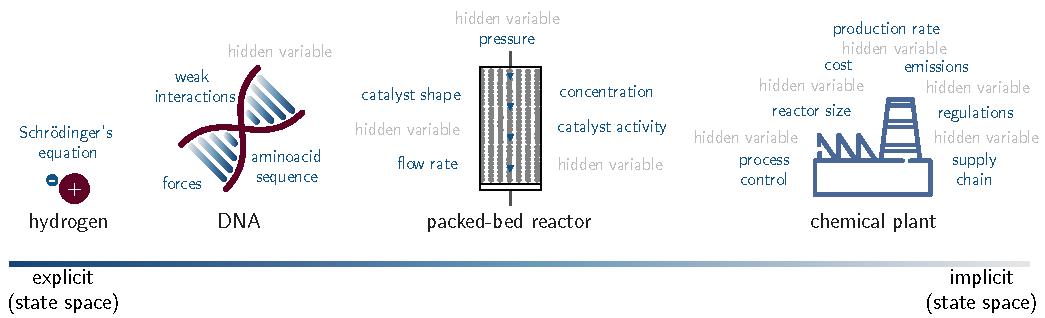
\includegraphics[width=1\textwidth]{figures/rescaled_figures/chemrev_figure1.pdf}   
    \caption{\textbf{State space description for chemistry at different scales}. We illustrate how the number of hidden variables (gray) is growing with scale and complexity. For simple systems we can explicitly write down all variables and their values and perfectly describe the system. For more complex systems---closer to practical applications---we can no longer do that. Many more variables cannot be explicitly enumerated.}
    \label{fig:shape_of_data}
\end{figure}

For phenomena characterized by irreducible complexity, success is often serendipitous. 
As pointed out by \textcite{rulev2017serendipity}, chemical literature commonly contains terms such as \enquote{to our surprise}, \enquote{remarkable reactivity}, or \enquote{unusual performance}, which may reflect the complexity of scientific questions and the diminishing explainability of observed results.

\paragraph{Emergent complexity} In contrast to irreducible complexity, there is a subset of chemical problems for which all relevant parameters can explicitly be listed, but the complexity emerges from the intricate, potentially chaotic, interactions among them. A well-known example is the Belousov-Zhabotinsky reaction, \autocite{Cassani2021BZ} which exhibits oscillations and pattern formation as a result of a complex chemical reaction network. 
Individual chemical reactions within the network are simple, but their interactions create a dynamic, self-organizing system with properties not seen in the individual components.
An example of how fast the parameter space can grow was provided by \textcite{NEURIPS2024_53704142}, who show that a single reaction type and a few hundred molecular building blocks can create tens of thousands of possible solutions. 
When scaling up to only five reaction types, the exploration of the entire space can become intractable, estimated at approximately $10^{22}$ solutions. 
When optimization objectives are involved---finding the shortest synthesis pathway or maximizing the yield---such problems are often NP-hard, meaning that no known polynomial-time algorithms can guarantee optimal solutions, though various heuristic and approximation methods can provide good solutions.

Knowing the ratio between explicit and implicit parameters helps in selecting the appropriate model architecture. 
If most of the variance is caused by explicit factors, these can be incorporated as priors or constraints in the model, thereby increasing data efficiency. 
This strategy can, for instance, be applied in the development of force fields where we know the governing equations and their symmetries, and can use them to enforce such symmetries in the model architecture (as hard restrictions to a family of solutions). \autocite{unke2021machine,Musil_2021}
However, when the variance is dominated by implicit factors, such constraints can no longer be formulated, as the governing relationships are not known. 
In those cases, flexible \glspl{gpm} with soft inductive biases---which guide the model toward preferred solutions without enforcing strict constraints on the solution space\autocite{wilson2025deep}---are more suitable. \glspl{llm} fall into this category.


\subsection{Scale of Chemical Data}
Chemistry is an empirical science in which every prediction bears the burden of proof through experimental validation.\autocite{zunger2019beware} 
However, there is often a mismatch between the realities of a chemistry lab and the datasets on which \gls{ml} models for chemistry are trained. 
Much of current data-driven modeling in chemistry focuses on a few large, structured, and highly-curated datasets where most of the variance is explicit (reducible complexity). 
Such datasets, \modelname{QM9} for example,\autocite{ramakrishnan2014quantum} often come from quantum-chemical computations.
Experimental chemistry, however, tends to have a significantly higher variance and a greater degree of irreducible complexity. 
In addition, since data generation is often expensive, datasets are small, and because science is about doing new things for the first time, many datasets also contain at least some unique variables.

Considering the largest chemistry text dataset, \modelname{ChemPile},\autocite{mirza2025chempile0} we can look at how the largest subsets fare in comparison to the smallest ones (see \Cref{tab:small_large_datasets}). 
The largest dataset is approximately three million times larger than the smallest one.

\begin{table}[!h]
    \centering
    \caption{\textbf{Token counts for the three largest and smallest datasets in the \modelname{ChemPile}\autocite{mirza2025chempile0} collection.} Dominating datasets contribute a large portion of the total token count (a token represents the smallest unit of text that a \gls{ml} model can process), with the small datasets significantly increasing the diversity.}
    \label{tab:dataset-sizes}
    \begin{tabular}{lr}
        \toprule
        \textbf{Dataset} & \textbf{Token count} \\
        \midrule
        \multicolumn{2}{l}{\textit{Three largest ChemPile datasets}} \\
        \midrule
        NOMAD crystal structures\autocite{scheidgen2023nomad} & 5,808,052,794 \\
        \gls{ord}\autocite{Kearnes_2021} reaction prediction & 5,347,195,320 \\
        \modelname{RDKit} molecular features & 5,000,435,822 \\
        \midrule
        \multicolumn{2}{l}{\textit{Three smallest ChemPile datasets}} \\
        \midrule
        Hydrogen storage materials\autocite{hymarcReversibleHydrides} & 1,935 \\
        List of amino-acids\autocite{alberts2002molecular} & 6,000 \\
        \gls{ord}\autocite{Kearnes_2021} recipe yield prediction& 8,372 \\
        \bottomrule
    \end{tabular}
    \label{tab:small_large_datasets}
\end{table}

The prevalence of many small, specialized datasets over large ones is commonly referred to as \enquote{the long tail problem}.\autocite{heidorn2008shedding} 


\begin{figure}[ht]
    \centering
    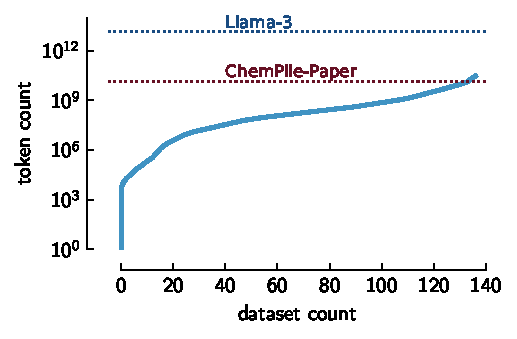
\includegraphics{figures/final_figures/2_DATA_cumulative_histogram.pdf}
    \caption{\textbf{Cumulative token count based on the \modelname{ChemPile} tabular datasets \autocite{mirza2025chempile0}}. We compare the approximate token count for three datasets: \modelname{Llama-3} training dataset,\autocite{grattafiori2024llama} openly available chemistry papers in the \modelname{ChemPile-Paper} dataset, and the \modelname{ChemPile-LIFT} dataset. As can be seen, by aggregating the collection of tabular datasets converted to text format in the \modelname{ChemPile-LIFT} subset, we can achieve the same order of magnitude as the collection of open chemistry papers. However, without smaller datasets, we cannot capture the breadth and complexity of chemistry data, which is essential for training \gls{gpm}. The tokenization method for both \modelname{ChemPile} and \modelname{Llama-3} is provided in the respective papers.}
    \label{fig:scale_of_data}
\end{figure}

This can be seen in \Cref{fig:scale_of_data}. We show that while a few datasets are large, the majority of the corpus consists of small but collectively significant and chemically diverse datasets.
The actual tail of chemical data is even larger, as \Cref{fig:scale_of_data} only shows the distribution for manually curated tabular datasets and not all data actually created in the chemical sciences.
Given that every dataset in the long tail relies on unique sources of variance---it is very difficult to leverage this long tail with conventional \gls{ml} techniques. However, the promise of \glspl{gpm} such as \glspl{llm} is that they can very flexibly integrate and jointly model the diversity of small datasets that exist in the chemical sciences.

\subsection{Dataset Creation}

Before a model can be trained or tested, suitable data must first be collected. 
It is important to note that when working with \glspl{gpm}, data can---but should not---be directly ingested in a raw format and requires some form of pre-processing.
Training \glspl{gpm} typically requires a large and diverse dataset, compiled in a form that can be efficiently ingested by the training pipeline.

Strategies for doing so can be broadly categorized into two groups (see  \Cref{fig:data_protocols}).
One can utilize a \enquote{top-down} approach where a large and diverse pool of data---e.g., results from web-crawled resources such as \modelname{CommonCrawl}\autocite{commoncrawl}---is filtered using custom-built procedures (e.g., using regular expressions or classification models). 
This approach is gaining traction in the development of foundation models such as \glspl{llm}.\autocite{penedo2023refinedweb,penedo2024fineweb,guo2025deepseek} Alongside large filtered datasets, various data augmentation techniques have further increased the performance of \glspl{gpm}.\autocite{maini2024rephrasing,pieler2024rephrasing}

Alternatively, one can take a \enquote{bottom-up} approach by specifically creating novel datasets for a given problem---an approach which has been very popular in \gls{ml} for chemistry. 

In practice, a combination of both approaches is often used. In most cases, key techniques include filtering and the generation of synthetic data.

\begin{figure}[ht]
    \centering
    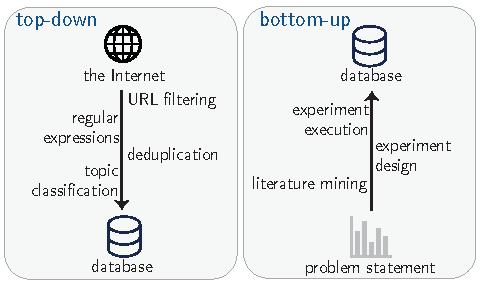
\includegraphics{figures/rescaled_figures/chemrev_figure3.pdf}
    \caption{\textbf{Dataset creation protocols}. In \enquote{top-down} approaches, we curate a large corpus of data, which can be used to train \glspl{gpm}. The \enquote{bottom-up} approach starts from a problem definition, and the dataset can be collected via literature mining and experiments. Both approaches can make use of synthetic data to increase the data size and diversity.}
    \label{fig:data_protocols}
\end{figure}


\subsubsection{Filtering}

\glspl{gpm} are currently trained on very large datasets, enabled by the availability of ever-growing computational resources.\autocite{krizhevsky2012imagenet,kaplan2020scaling, hooker2020hardware, dotan2019value0laden} 
The Internet has been the primary source of dataset construction for \glspl{gpm}. 
While initially the focus was on training on maximally large datasets, empirical evidence has shown that smaller, higher-quality datasets can lead to better results.\autocite{gunasekar2023textbooks, marion2023less} For example, \textcite{shao2024deepseekmath0} filtered \modelname{CommonCrawl} for mathematical text using a combination of regular expressions and a custom, iteratively trained classification model\autocite{bojanowski2017enriching}. 
An alternative approach was pursued by \textcite{thrush2024improving} who introduced a training-free framework. In this method, the pre-training text was chosen by measuring the correlation of each web-domain's perplexity (a metric that measures how well a language model predicts a sequence of text)---as scored by $90$ publicly-available \glspl{llm}---with downstream benchmark accuracy, keeping only the high-correlation domains. 

In the chemical domain, \modelname{ChemPile}\autocite{mirza2025chempile0} is the only open-source, pre-training scale dataset, that underwent several filtering steps. For example, a large subset of the papers in \modelname{ChemPile-Paper} come from the \modelname{Europe PMC} dataset. To filter for chemistry papers, a custom classification model was trained from scratch using topic-labeled data from the \modelname{CAMEL}\autocite{li2023camel} dataset. To evaluate the accuracy of the model ($\text{F1-score}=0.77$), expert-annotated data was used.


\subsubsection{Synthetic Data}
\label{sec:syn-data}

Instead of only relying on existing datasets, one can also leverage techniques for generating synthetic data. 
Generation of synthetic data is often required to augment scarce real-world data, but can also be used to achieve the desired model behavior (e.g., invariance in image-based models).

These approaches can be grouped into rule-based and generative methods. 
Rule-based methods apply manually defined transformations---such as rotations and mirroring---to present different representations of the same instance to a model. 
In contrast, generative augmentation creates new data by applying transformations learned through a \gls{ml} model.

\paragraph{Rule-based augmentation} The transformations applied for generating new data in rule-based approaches vary depending on the modality (e.g., image, text, or audio).  
The most common application of rule-based techniques is on images, via image transformations such as distortion, rotation, blurring, or cropping.\autocite{shorten2019survey} 
In chemistry, tools like \modelname{RanDepict}\autocite{brinkhaus2022randepict} have been used to create enriched datasets of chemical representations. 
These tools generate human-like drawings of chemical structures that mimic the common illustrations found in scientific literature or even in patents (e.g., by applying image templates from different publishers, or emulating the style of older manuscripts) and further augment them using conventional image-augmentation techniques.


Rule-based augmentations can also be applied to text. Early approaches involved simple operations like random word swapping, random synonym replacement, and random deletions or insertions, which are often labeled \enquote{easy augmentation} methods.\autocite{shorten2021text,wei2019eda0}

In chemistry, text templates have been used.\autocite{xie2023darwin,mirza2025chempile0, jablonka2024leveraging, vanherck2025assessment}  
Such templates define a sentence structure with semantically configurable fields, which are then filled using structured tabular data. 
However, it is still unclear how to best construct such templates, as studies have shown that the same data shown in different templates can lead to distinct generalization behavior.\autocite{gonzales2024evaluating} 

We can also apply rule-based augmentation for specific molecular representations (for more details on representations see \Cref{sec:common_representations}). 
For example, the same molecule can be represented with multiple different, yet valid \gls{smiles} strings. 
% The use of all of them can be leveraged to obtain richer latent representations compared to models trained only on canonical \gls{smiles}. 
\textcite{bjerrum2017smiles} used this technique to augment a predictive model, where multiple \gls{smiles} strings were mapped to a single property. 
When averaging the predictions over multiple \gls{smiles} strings, at least a $10\%$ improvement was observed compared to their single \gls{smiles} counterparts. 
Such techniques can be applied to other molecular representations (e.g., \gls{iupac} names or \gls{selfies}), but historically, \gls{smiles} has been used more often. 
As a result, its augmentations have been studied more extensively.\autocite{kimber2021maxsmi,born2023chemical,arus2019randomized}

A broad array of augmentation techniques has been applied to spectral data---from simple noise addition\autocite{ke2018convolutional,moreno2022application} to physics-informed augmentations (e.g., through DFT simulations).\autocite{oviedo2019fast,gao2020general}

\paragraph{Generative augmentation}
In some cases, however, it is not possible to write down the rules. For instance, it is not obvious how text can be transformed into different styles using rules alone.
Recent advances in deep learning have facilitated another, more flexible, approach to synthetic data generation. \autocite{maini2024rephrasing} 
A simple technique is to apply contextual augmentation \autocite{kobayashi2018contextual}, which implies the sampling of synonyms from a probability distribution of a \gls{lm}. 
Another technique is \enquote{back translation},\autocite{edunov2018understanding} a process in which text is translated to another language and then back into the original language to generate semantically similar variants. 
While this technique is typically used within the same language,\autocite{lu2024mathgenie0} it can also be extended to multilingual setups\autocite{hong2024cantonmt0}.
 
Other recent approaches have harnessed auto-formalization\autocite{NEURIPS2022_d0c6bc64}, a \gls{llm}-powered approach that can turn natural-language mathematical proofs into computer-verifiable mathematical languages such as \modelname{Lean}\autocite{de2015lean} or \modelname{Isabelle}\autocite{wenzel2008isabelle}. 
Such datasets have been utilized to advance mathematical capabilities in \glspl{lm}.\autocite{xin2024deepseek,trinh2024solving}

A drawback of generatively augmented data is that its validity is cumbersome to assess at scale, unless it can be verified automatically by a computer program. 
For example, it was demonstrated that an increasing ratio of synthetic data can facilitate model collapse.\autocite{kazdan2024collapse,shumailov2024ai}

Having reviewed the data sources and generation methods, we will, in the following, discuss architectures and training approaches for \glspl{gpm}.  
%\newpage
\section{Building Principles of GPMs}

\subsection{Taxonomy of Foundation Models}
\label{sec:taxonomy}

In this review, we focus on \glspl{gpm}, which are commonly trained on vast, often unstructured datasets and are able to generalize to new tasks easily.
Currently, \glspl{llm} are the most prominent members of the \gls{gpm} family, but many of the principles discussed here are transferable across different types of \glspl{gpm}, and we will use the term \gls{gpm} to highlight these general applications.

\Glspl{gpm} can efficiently operate in the low-data regime. 
In contrast to conventional transfer learning where a model is pre-trained on a task and then adapted to a slightly modified task through fine-tuning, we often do not need to change the weights of a \gls{gpm}, since the model can adapt to new problems at inference time through techniques such as \gls{icl}\autocite{brown2020language} or \gls{rag} (see \Cref{sec:model_adaptation}).\autocite{lewis2020retrieval}

\glspl{gpm} are not chemistry-specific models. 
They are models for general use that leverage cross-domain information.
Chemistry is deeply intertwined with other scientific fields, including physics, biology, and mathematics. 
Being able to access all this knowledge at inference time can be critical.
In addition, there is a compelling argument to be made for \glspl{llm}:  natural language has evolved to represent all concepts that humans can ponder. Thus, leveraging natural language might be a very productive way to approach scientific discovery.  
Furthermore, \glspl{gpm} can be integrated with problem-solving tools (\Cref{sec:agents}). 
Such systems are typically described as being \emph{agentic} and are key to further automation and integration of \gls{ai} systems in the real world. 

In the following, we discuss how such models work and can be trained.

\subsection{Representations}
To interact with any machine, we need to convert the input into numeric values. At its core, all information within a computer is represented as bits (zeros and ones). 
Bits are grouped into bytes (8 bits), and meaning is assigned to these sequences through encoding schemes like \texttt{ASCII} or \texttt{UTF-8}. 
Everything---text, a pixel in an image, or even a chemical structure---can be stored as sequences of bytes. 
For example, \enquote{\ce{H2O}} can be translated into the byte sequence, \enquote{H}, \enquote{2}, \enquote{O}. 
However, using raw byte sequences for \gls{ml} presents significant computational inefficiency as representing chemical entities requires long byte sequences, and models would need to learn complex mappings between arbitrary byte patterns and their meanings (as the encoding schemes are not built around chemical principles). 
Furthermore, handling variable-length sequences can pose additional challenges for models, as they may struggle to perform well on unseen inputs. \autocite{zhou2023algorithms,baillargeon2022assessing} 

A more efficient mapping that is built on top of the underlying byte representation is \gls{ohe}. 
Instead of working with variable-length byte sequences, we create a fixed vocabulary (\{\ce{H2O}, \ce{CO2}, \ce{HCl}\}) where each discrete category (in this case, molecule) gets a unique vector: \ce{H2O} becomes [1, 0, 0], \ce{CO2} becomes [0, 1, 0], and so on. 
This provides unambiguous, computationally manageable representations. 
As the number of categories grows, one-hot vectors become increasingly long and sparse, making them computationally inefficient---particularly for large vocabularies, i.e., many categories.
For example, we need a vocabulary of size 118 to model only the unique elements in the periodic table. 
Now, imagine the vocabulary required for all unique compounds---the size combinatorially explodes. 
More importantly, while \gls{ohe} distinguishes molecules or elements, it still treats them as entirely independent. 
It does not capture any properties of the entity it represents. For example, the ordering of numbers (such as $4<5$) or chemical similarities (such as \ce{Cl} being more similar to \ce{Br} but less similar to \ce{Na}) would not be preserved. \autocite{chuang2018comment}
Embeddings (learned encoding), that we will discuss in \Cref{sec:embeddings}, solve this through learned, dense vector representations.

\subsubsection{Common Representations of Molecules and Materials}
\label{sec:common_representations}

Before any chemical entity can be converted into a numerical vector---whether through simple \gls{ohe} or complex learned embeddings---it must first be described in a standardized format (for example, if we are working with materials, it should be able to encode all materials), which is then mapped to encodings. 

For complex entities like molecules, materials, and reactions, this choice of what fundamental units to represent  (\enquote{should we include only atomic numbers?}, \enquote{Should we include something about the structure?}, etc.) is among the most consequential decisions in building a model. 
It determines the inductive biases---the set of assumptions that guide learning algorithms toward specific patterns over others. 
The landscape of chemical representations reflects different answers to this question, each making distinct trade-offs between simplicity, expressiveness, and computational efficiency.


\begin{longtable}{%
  >{\raggedright\arraybackslash}p{0.20\textwidth}
  >{\raggedright\arraybackslash}p{0.15\textwidth}
  >{\raggedright\arraybackslash}p{0.25\textwidth}
  >{\raggedright\arraybackslash}p{0.32 \textwidth}
}
  \caption{\textbf{Comparison of common molecular representations}. For the encoded information contained by each representation, we followed the criteria used by \textcite{alampara2024mattext}. The examples shown are \textit{aspirin} for elemental composition, \gls{iupac} name, \gls{smiles}, \gls{selfies}, \glslink{inchi}{InChI}, graphs, 3D coordinates; and \textit{silicon} for \glslink{cif}{CIF}, condensed \glslink{cif}{CIF}, \glslink{slices}{SLICES}, \glslink{localenv}{Local-Env}, and natural-language description. Two non-canonical \gls{smiles} are shown to illustrate ambiguity. The examples for 3D coordinates, \glslink{cif}{CIF}, and natural-language description are truncated to fit in the table. For the multimodal representation, only one of the possible modalities is shown ($^{13}$C \glslink{nmr}{NMR} spectrum).}
  \label{tab:molecular-representations} \\
  \toprule
  \textbf{Representation} & \textbf{Encoded information} & \textbf{Description} & \textbf{Example} \\
  \midrule
  \endfirsthead

  \multicolumn{4}{c}%
  {\tablename\ \thetable{} — continued from previous page} \\
  \toprule
  \textbf{Representation} & \textbf{Encoded info} & \textbf{Description} & \textbf{Example} \\
  \midrule
  \endhead

  \midrule
  \multicolumn{4}{r}{Continued on next page} \\
  \endfoot


  \bottomrule
  \endlastfoot
    Elemental composition & Stoichiometry & Always available, but non-unique. & C9H8O4 \\
    \addlinespace
    \gls{iupac} name & Stoichiometry, bonding, geometry & Universally understood, systematic nomenclature, unmanageable for large molecules, and lacks detailed 3D information. & 2-acetyloxybenzoic acid \\
    \addlinespace
    \gls{smiles} \autocite{weininger1988smiles} & Stoichiometry, bonding & Massive public corpora and tooling support, however, there are several valid strings per molecule, and it does not contain spatial information. & \footnotesize \makecell[tl]{%
    \smi{CC(=O)OC1=CC=CC=C1C(=O)O}\\[10pt]      % blank line = 4 pt
    \smi{O=C(O)c1ccccc1OC(C)=O}\\[10 pt]
    \emph{etc.}
    } \\
    \addlinespace
    \gls{selfies} \autocite{krenn2020self,cheng2023group} & Stoichiometry, bonding & 100\% syntactic and semantic validity by construction, including meaningful grouping. & \footnotesize \texttt{[C][C][=Branch1][C][=O][O]} \texttt{[C][=C][C][=C][C][=C]} \texttt{[Ring1][=Branch1][C]} \texttt{[=Branch1][C][=O][O]} \\
    \addlinespace
    \gls{inchi} & Stoichiometry, bonding & Canonical one-to-one identifier; encodes stereochemistry layers. & \footnotesize \texttt{InChI=1S/C9H8O4/c1-6(10)13} \texttt{-8-5-3-2-4-7(8)9(11)12/} \texttt{h2-5H,1H3,(H,11,12)} \\
    \addlinespace
    Graphs & Stoichiometry, bonding, geometry & Strong inductive bias that works with \glspl{gnn}. Symmetry-equivariant variants available. Long-range interactions are implicit. & \cellimage{figures/Aspirin.png} \\
    \addlinespace
    xyz representation & Stoichiometry, geometry & Exact spatial detail. It is high dimensional, and orientation alignment is needed. & \footnotesize 1.2333    0.5540    0.7792 O -0.6952   -2.7148   -0.7502 O 0.7958   -2.1843    0.8685 O 1.7813    0.8105   -1.4821 O -0.0857    0.6088    0.4403 C \ldots \\ % -0.7927   -0.5515    0.1244 C -0.7288    1.8464    0.4133 C -2.1426   -0.4741   -0.2184 C -2.0787    1.9238    0.0706 C -2.7855    0.7636   -0.2453 C -0.1409   -1.8536    0.1477 C 2.1094    0.6715   -0.3113 C 3.5305    0.5996    0.1635 C -0.1851    2.7545    0.6593 H -2.7247   -1.3605   -0.4564 H -2.5797    2.8872    0.0506 H -3.8374    0.8238   -0.5090 H 3.7290    1.4184    0.8593 H 4.2045    0.6969   -0.6924 H 3.7105   -0.3659    0.6426 H -0.2555   -3.5916   -0.7337 H \\
    \addlinespace
    Multimodal & Stoichiometry, bonding, geometry, symmetry, periodicity, coarse graining & Combines complementary signals; boosts robustness and coverage. It is hard to implement, the complexity scales with the amount of representations, some modalities are data-scarce, and the information encoded totally depends on the modalities included. & \cellimage{figures/60031761.jpeg} \\
    \addlinespace
    \gls{cif} \autocite{hall1991crystallographic} & Stoichiometry, bonding, geometry, periodicity & Standardized and widely supported, however, it carries heterogeneous keyword sets and parser overhead & \footnotesize \texttt{data\_Si \_symmetry\_space\_group\_name\_H-M   'P 1' \_cell\_length\_a   3.85 \ldots \_cell\_angle\_alpha   60.0 \ldots \_symmetry\_Int\_Tables\_number   1 \_chemical\_formula\_structural   Si \_chemical\_formula\_sum   Si2 \_cell\_volume   40.33 \_cell\_formula\_units\_Z   2 loop\_ \_symmetry\_equiv\_pos\_site\_id  \_symmetry\_equiv\_pos\_as\_xyz   1  'x, y, z' loop\_ \_atom\_type\_symbol \_atom\_type\_oxidation\_number  Si0+  0.0loop\_ \_atom\_site\_type\_symbol \_atom\_site\_label \_atom\_site\_symmetry\_multiplicity \_atom\_site\_fract\_x \ldots \_atom\_site\_occupancy  Si0+  Si0  1  0.75  0.75  0.75  1.0 Si0+  Si1  1  0.0  0.0  0.0  1.0}\\ 
    \addlinespace
    Condensed \gls{cif} \autocite{gruver2024finetuned, antunes2024crystal} & Stoichiometry, geometry, symmetry, periodicity & Good for crystal generation tasks. It omits occupancies and defects, custom tooling is needed, and only works for crystals & \footnotesize \texttt{3.8 3.8 3.8 59 59 59 Si0+ 0.75 0.75 0.75 Si0+ 0.00 0.00 0.00}\\
    \addlinespace
    \glslink{slices}{SLICES} \autocite{Xiao_2023} & Stoichiometry, bonding, periodicity & Invertible, symmetry-invariant and compact for general crystals. However, it carries ambiguity for disordered sites & \footnotesize \texttt{Si Si 0 1 + + + 0 1 + + o 0 1 + o + 0 1 o + +}   \\
    \addlinespace
    \glslink{localenv}{Local-Env}\autocite{alampara2024mattext} & Stoichiometry, bonding, symmetry, coarse graining & Treats each coordination polyhedron as a \enquote{molecule}, it is transferable and compact; but it ignores long-range order and its reconstruction requires post-processing & \footnotesize \texttt{R-3m Si (2c) [Si][Si]([Si])[Si]} \\
    \addlinespace
    Natural-language description \autocite{ganose2019robocrystallographer} & Stoichiometry, bonding, geometry, symmetry, periodicity, coarse graining & It is human-readable and tokenizable in a meaningful way by pretrained \glspl{llm}. However, trying to encode all the information can lead to verbose, ambiguous descriptions. & \enquote{Silicon crystallizes in the diamond-cubic structure, a lattice you can picture as two face-centred-cubic frameworks gently interpenetrating\ldots} \\
\end{longtable}

However, a common strategy is to represent chemical information as a sequence of characters. This allows us to leverage architectures initially designed for natural language. 
This approach has found particular success in language modeling for predicting protein structures and functions, where the amino acid sequence, the very foundation of a protein's structure and function, is easily represented as text.\autocite{Rives_2021, Elnaggar_2022, Ruffolo_2024}
The most prevalent string representation for molecules in chemistry is \gls{smiles}\autocite{weininger1988smiles}. \gls{smiles} strings essentially provide a linear textual representation of a molecular graph, including information about atoms, bonds, and rings. 
However, \gls{smiles} representations have significant limitations. 
The same molecule can have multiple valid \gls{smiles} strings (so-called non-canonical representations).
Although the existence of non-canonical representations enables data augmentation (see \Cref{sec:syn-data}), it can also confuse models because the same molecule would have different encodings, each one originating from a different \gls{smiles} string. 
In addition, \gls{smiles} imposes a relatively weak inductive bias; the model must still learn the complex rules of valence and bonding from the grammar of these character sequences. Moreover, \gls{smiles} does not preserve locality: structural motifs that are directly bonded or physically close to each other in a molecule, can be very far apart in the \gls{smiles} representation.
Nevertheless, \gls{smiles} is widely used owing to its popularity and the amount of data present in different places (internet, papers, databases) using this representation. 

A limitation of \gls{smiles} is that not every \gls{smiles} string corresponds to a valid molecule.
A more robust alternative is \gls{selfies}\autocite{krenn2020self,cheng2023group}, where every \gls{selfies} corresponds to a valid molecule, providing a stronger bias towards chemically plausible structures (chemical validity biases). 
The \gls{inchi} is another standardized string representation. 
Unlike \gls{smiles}, \gls{inchi} strings, as identifiers, are canonical---each molecule has exactly one \gls{inchi} representation.  
This eliminates ambiguity, but comes at the cost of human readability and increased string length. 

In the realm of materials, no natural representation has emerged.  
Previous work has indicated that for certain phenomena (e.g., when all structures in a dataset are in the ground state), composition might implicitly encode geometric information \autocite{tian2022information, Jha_2018, Wang_2021}. 
Material composition alone can be predictive of various material properties and is a widely chosen method to represent materials, depending on the task. 
When structural information is available, \glspl{cif}, initially proposed as a standard way to archive structural data in crystallography \autocite{hall1991crystallographic}, is now a widely used representation. \textcite{gruver2024finetuned, antunes2024crystal} proposed a condensed version of \glspl{cif}, which includes only the parameters necessary for building the crystal structure in a crystal generation application. \textcite{ganose2019robocrystallographer} aimed to create human-readable descriptions by proposing a tool to generate natural-language descriptions of crystal structures automatically. 
For specific material classes, such as \glspl{mof}, specialized representations like \modelname{MOFid} \autocite{Bucior_2019} have been developed. 


Instead of a string, we can represent chemical substances as graphs. 
Here, we are directly encoding atoms (nodes) and bonds (edges). 
This representation 
introduces a much stronger inductive bias: locality biases that explicitly inform the model about atomic connectivity, so the model does not need to learn this fundamental principle from scratch. Symmetry has been incorporated into many of the best-performing graph-based approaches by designing invariant or equivariant representations \autocite{Langer_2022, Musil_2021} and architectures \autocite{satorras2021n, Batzner_2022}. 
These approaches are efficient in capturing strong symmetry-related inductive biases along with the topology of locality biases. 

The optimal choice of representation depends on the specific application. For applications where precise 3D structure matters, such as protein-ligand docking, geometric representations become essential.
For \glspl{gpm}, a more natural choice would be text, to take advantage of the better overlap with the pre-training corpus and also to interact with humans. 
Ultimately, weaker inductive biases (like text) offer greater flexibility and can capture unexpected patterns, but may require more data to learn the fundamental rules. 
The successful design of inductive biases requires balancing domain knowledge with learning flexibility. 
Stricter inductive biases (like graphs) incorporate more domain knowledge, leading to greater data efficiency but potentially limiting the model's ability to discover patterns that contradict our initial assumptions. 

Beyond choosing a single optimal representation, modern \gls{ml} allows for the simultaneous use of multiple representations. 
A chemical entity can be described not only by its textual \gls{smiles} string or its connectivity graph, but also by its experimental spectra (e.g., \gls{nmr}, \gls{ir}), or even a microscopy image. 
Each of these modalities provides a complementary layer of information. 
A more detailed section on using multiple representations is presented in \Cref{sec:multimodal_chem}


\subsubsection{Tokenization}
Once we have chosen a representation format---whether \gls{smiles} strings, \gls{cif} files, or chemical formulas---we face another fundamental question: How does a model process these variable-length sequences of characters? 
One might imagine creating a unique identifier or encoding for every single molecule or string. 
It is impractical to have a dictionary entry for every sentence in a language due to the similar scaling problems of \gls{ohe}.

Consider the molecule with the \gls{smiles} string \texttt{CN1C=NC=C1C(=O)}. 
We could break down the representation in several different ways: as individual characters (\texttt{C}, \texttt{N}, \texttt{1}, \texttt{C}, \texttt{=}, etc.), as atom-bond pairs (\texttt{CN}, \texttt{C=}, \texttt{NC}), or as chemically meaningful fragments (\texttt{CN1}, \texttt{C=NC}, etc.). 
Each choice creates a different \enquote{language} for the model to learn, with distinct computational and learning implications.

This is where tokenization becomes essential. 
It is the strategy of breaking down a complex representation (like a \gls{smiles} string) into a sequence of discrete, manageable units called tokens. The core idea is to find a set of common, reusable building blocks. Instead of learning about countless individual molecules, the model knows about a much smaller, finite vocabulary of these tokens. By learning an encoding for each token, the model gains the ability to understand and construct representations for an immense number of molecules---including those it has never seen before---by combining the meanings of their constituent parts. 
This compositional approach enables powerful generalization.

The concept of tokenization, or defining the fundamental units of input, extends beyond string-based representations. 
In images, it could be patches of images. 
In graph-based models, the analogous decision is how to define the features for each node (atom) and edge (bond). 
Should a node simply represent an atomic number (a simple \enquote{token}), or should it be a more complex sub-structure like a structural motif\autocite{bouritsas2022improving} (a richer \enquote{token})? This choice determines the level of chemical knowledge initially provided to the model. 
Ultimately, the tokenization strategy defines the elementary units for which the model will learn embeddings, setting the stage for learning the powerful and context-aware representations discussed next.


\subsubsection{Embeddings} \label{sec:embeddings}

Through training, models can learn to map discrete inputs into continuous spaces where similar items have meaningful relationships (for example, similar items cluster in this continuous space). 
In the simplest approach, they can be created by training models (so-called \modelname{Word2Vec} models) that take one-hot encoded inputs and predict the probability of words in the context.\autocite{mikolov2013efficient, mikolov2013distributed, Tshitoyan_2019}
Embeddings are powerful because they learn relationships between entities, allowing for the efficient compression of data and the uncovering of hidden patterns that would otherwise be invisible in the raw data.

The advent of \glspl{gpm} has further underscored the usefulness of high-quality embeddings. 
These models, trained on vast amounts of chemical data, learn to create powerful, generalizable embeddings that can be adapted to a wide range of downstream tasks, from property prediction (see \Cref{sec:prediction}) to molecular generation (see \Cref{sec:mol_generation}). 
The choice of embedding strategy often depends on the specific problem at hand. 
In the following sections, we describe the process of generating, refining, and using these embeddings through training and different architectures.


\subsection{General Training Workflow}

The entire training process of a \gls{gpm} typically contains multiple steps that can be divided into two broad groups (see \Cref{fig:training_workflow}). \autocite{howard2018universal} 
The first step is pre-training, which is usually done in a self-supervised manner and focuses on learning a data distribution---the underlying set of rules and patterns that make up the data. 
Imagine all possible arrangements of atoms, both real and unfeasible. 
The data distribution describes which molecules are \enquote{likely} (stable, following chemical rules) and which are \enquote{unlikely} or \enquote{impossible} (random assortments of atoms).


\begin{figure}[!ht]
    \centering
    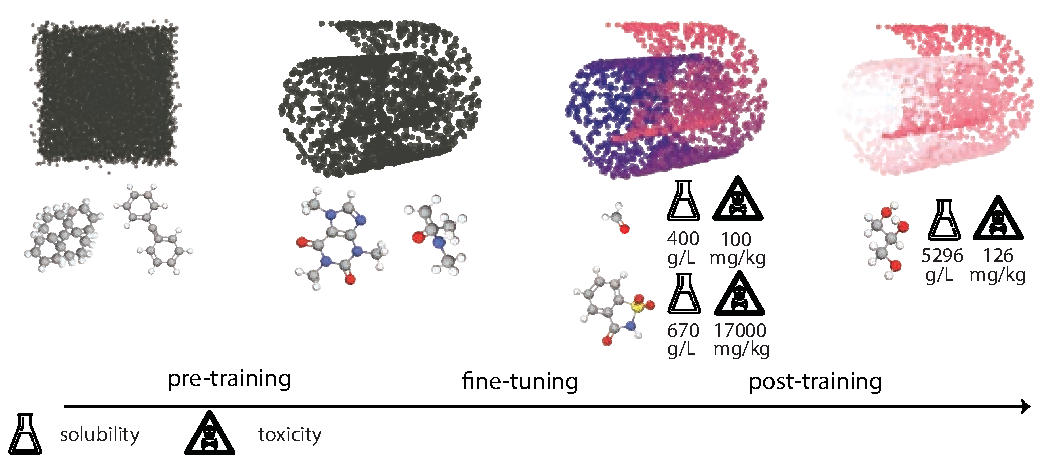
\includegraphics[width=1\textwidth]{figures/rescaled_figures/chemrev_figure4.pdf}
    \caption{\textbf{General training workflow through the lens of molecular science}. The figure illustrates the progression from pre-training through fine-tuning to post-training stages.  \textbf{(1) Pre-training:} The model learns the underlying data distribution from a vast, unlabeled dataset. This is visualized as transforming an unstructured representation space (left, square cloud) into a structured manifold (the Swiss roll). At this stage, the model has learned the \enquote{shape} of the data: the fundamental rules that make a molecule chemically valid. However, the representations are not yet specialized for any task. 
    \textbf{(2) Fine-tuning:} The model is trained on specific, labeled tasks, such as predicting solubility (flask icon) and toxicity (skull icon). This process \enquote{colors} the manifold, adjusting the learned representations so that their position now also correlates with specific properties (e.g., blue for one property profile, red for another). 
    \textbf{(3) Post-training Alignment:} The model's behavior is biased towards desired outcomes. This is visualized as preferentially sampling from a specific region of the colored manifold, such as generating molecules predicted to have high solubility and low toxicity (right, the brighter red region).}
    \label{fig:training_workflow}
\end{figure}


 Pre-training a model is teaching it to recognize this pattern. 
 By observing millions of valid examples, the model learns the \enquote{grammar} of chemistry---the principles that make a molecule physically plausible. 
 A model that has successfully learned the distribution can distinguish a valid structure from noise and can even generate new, chemically sensible examples, much like someone who has learned the rules of a language can form new, grammatically correct sentences.  

A model does not learn the data distribution by storing an explicit formula. Instead, during pre-training (see \Cref{sec:pretraining} for more details), it learns to create an internal representation---an embedding (see \Cref{sec:embeddings}).
The training process guides the model to map inputs to these embeddings in a structured manner, forming a high-dimensional space, where representations of similar, valid inputs are clustered together.


The second step is post-training, also called fine-tuning, in which the model is adapted to learn task-specific labels and capabilities, essentially \enquote{coloring} the learned structure with domain-specific knowledge. 
Crucially, fine-tuning does not discard the learned distribution but refines it. 
As shown in \Cref{fig:training_workflow}, the fundamental shape of the manifold (the Swiss roll) is preserved. 
The \enquote{coloring} process corresponds to adjusting the internal representations so they now also encode task-specific properties. 
For example, the model learns to map molecules with high solubility to one region of the manifold (e.g., the red area) and those with high toxicity to another. 
The representation of each molecule is thus enriched, now containing information not just about its structural validity but also about its properties.

Finally, techniques such as \gls{rl} are used to align the model's outputs with preferred choices. 
This step further refines the learned distribution by biasing the model's sampling behavior to favor specific modes of the distribution. 
In terms of the representation space, the model learns to prioritize generating or paying attention to points in desirable regions. As depicted in the post-training panel of \Cref{fig:training_workflow}, this biases the output towards a specific section of the colored manifold---in this case, perhaps molecules with high solubility (the brighter pink region).



\subsection{Pre-training: Learning the Shape of Data}
\label{sec:pretraining}

Pre-training establishes the foundational knowledge and capabilities of the model. 
During pre-training, the model learns general patterns, relationships, and structures from massive datasets (often trillions of tokens, see \Cref{fig:scale_of_data}). 
The model learns to map input to internal representations or features through so-called \gls{ssl} objectives like reconstructing corrupted inputs (predicting masked tokens, or predicting future sequences, see \Cref{sec:ssl}). 

This large-scale pre-training allows models to capture rich representations of the statistical distributions inherent to the data.  These learned distributions capture the fundamental patterns and structure of the domain (scientific language grammar, physical and chemical principles that govern materials). \Cref{fig:training_workflow} illustrates the distribution captured, from an uninstructed manifold prior to pre-training (if you randomly pick from this manifold, you get noise or non-physical molecules) to a structured manifold, where if you sample from this distribution (the black Swiss roll) you get a valid molecule.
For example, the model might learn commonly occurring structures, scientific notations, and scientific terms. 
Furthermore, it might construct hierarchical relationships between these concepts, such as those between chemical compounds, elements, and their properties.  
This distributional learning empowers the model to make predictions about new examples by understanding their relation to the learned patterns. Crucially, this ability stems from the development of transferable features, rather than mere data memorization \autocite{brown2020language}. 

As illustrated by the Swiss roll in \Cref{fig:training_workflow}, the pre-training process creates a structured manifold where invalid inputs are mapped far away. Therefore, learning high-quality representations is the concrete computational method for capturing the abstract statistical distribution of the data; the structure of this representation space is the model's learned approximation of the data's true shape.

\subsubsection{Self-Supervision} \label{sec:ssl}

\glspl{ssl} allows models to learn from unlabeled data by generating \enquote{pseudo-labels} from the data's structure. 
The original, unlabeled data serves as its own \enquote{ground truth}. 
This differs significantly from supervised learning, a traditional method where models are trained using labeled datasets. 
In supervised learning, each piece of data is explicitly tagged with the correct output, which the model then learns to predict. 
Such manual labeling is often an expensive, time-consuming, and domain-specific process. 
\glspl{ssl} has emerged as a particularly effective strategy for pre-training \glspl{llm}, since natural-language corpora are abundant but rarely annotated. 
Proxy strategies have then been applied to other types of model architectures as well. 
The ability to extract structure from data \textit{without labels} is a key enabler for foundation models and underpins the pre-training phase.

\subsubsection{Families of Self-Supervised Learning}

\gls{ssl} encompasses a variety of approaches. While distinct methods exist, they can be grouped into broader families based on their underlying principles. \Cref{fig:types_ssl} illustrates the two main families: generative and contrastive, along with example pretext tasks for each.

\begin{figure}[H]
    \centering
    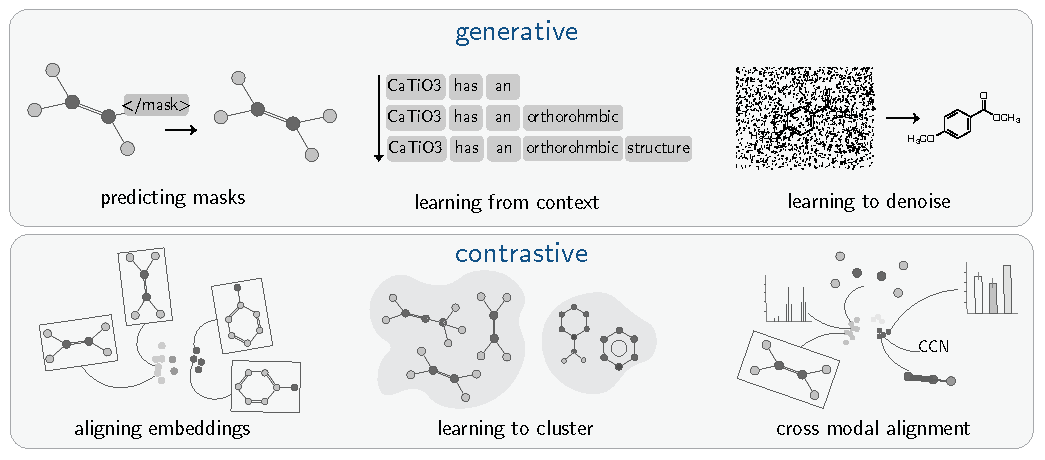
\includegraphics[width=1\textwidth]{figures/rescaled_figures/chemrev_figure5.pdf}
    \caption{\textbf{Main families in \glspl{ssl}}. The figure illustrates the two primary approaches to \gls{ssl}, each using different strategies to generate pseudo-labels from the data itself.
    \textbf{Generative Methods (Top Panel):} This family focuses on reconstruction and prediction. The model learns representations by generating missing information. Examples shown correspond to the pretext tasks discussed in the text: (1) \textit{Predicting masks} in a graph, analogous to masked modeling (more details in \Cref{sec:masked_modeling}); (2) \textit{Learning from context}, which is the basis for next token prediction (more details in \Cref{sec:next_token_prediction}); and (3) \textit{Learning to denoise}, where the model reconstructs a clean input from a corrupted version. (see \Cref{sec:denoising})
    \textbf{Contrastive Learning (Bottom Panel):} This family learns by comparing samples. The model is trained to pull representations of similar samples together while pushing dissimilar ones apart. Examples include: (1) \textit{Aligning embeddings} from different augmentations of the same molecule, a core idea in Instance Discrimination (more details in \Cref{sec:instance_discrimination}); (2) \textit{Learning to cluster} similar molecules together, as in Clustering-based Contrastive Learning (see \Cref{sec:clustering_cl}); and (3) \textit{Cross-modal alignment}, where representations from different data types (e.g., a molecule's graph and its spectral properties) are learned jointly. (see \Cref{sec:contrastive_learning} )}
    \label{fig:types_ssl}
\end{figure}

\subsubsection{Generative Methods}

This family of methods focuses on learning representations by reconstructing or predicting parts of the input data from other observed parts. 
The model learns the underlying data distribution by learning to re-generate the missing information. 
Examples shown in \Cref{fig:types_ssl} include predicting masked portions of a graph, learning from surrounding text context, and learning to denoise an image.

\label{sec:masked_modeling}
\paragraph{Masked Modeling}  In this method, portions of the input data are intentionally obscured or \enquote{masked}. The model's primary objective is then to reconstruct these hidden segments accurately. \autocite{devlin2018bert0} 
This process can be conceptualized as a \enquote{fill-in-the-blanks} task, compelling the model to infer missing information from its context. This enables the model to develop a deep understanding of contextual dependencies of data's structure and semantics without requiring explicit human-labeled annotations. For chemical data, this could involve masking and predicting tokens in \glspl{smiles}/\glspl{selfies} strings \autocite{chithrananda2020chemberta, zhang2025scientific} (i.e., hiding atoms and training the model to guess what is missing), omitting atom or bond types in molecular graphs \autocite{mahmood2021masked,wang2022molecular, reiser2022graph}, removing atomic coordinates in 3D structures, or masking sites within a crystal lattice.



\paragraph{Next Token Prediction} 
\label{sec:next_token_prediction}
Many forms of data, such as text, can be represented as sequences of tokens. 
One of the most powerful \gls{ssl} tasks for such sequential data is next-token prediction.
Here, the core objective is for a model to anticipate and generate the subsequent token in a given sequence, based on the contextual information provided by preceding tokens. 
Because text unfolds naturally in a sequence, it offers the reference information the model needs in order to learn. This approach has been applied to chemical and material representations by treating molecular string representations (\glspl{smiles}, \glspl{selfies}, etc.) or material representations as sequences \autocite{adilov2021generative, wang2023cmolgpt, schwaller2019molecular, alampara2024mattext}. 
During training, the model constantly adjusts itself to maximize the likelihood (trying to make good predictions more probable and bad predictions less probable). In this context, likelihood refers to the probability of observing the actual subsequent token given the preceding tokens in the sequence . This is accomplished by making each prediction based on the preceding input, which establishes the conditional context (see \Cref{eq:nexttoken}).


\begin{tcolorbox}[
    title= Cross-Entropy Loss,
    breakable,
    enhanced,
    colback=white,
    colframe=black!30,
    colbacktitle=black!10,
    coltitle=black,
    fonttitle=\bfseries,
    boxrule=0.5mm,
    left=2mm,
    right=2mm,
    top=4mm,
    bottom=4mm,
    middle=10mm
]
\label{eq:nexttoken}
\begin{center}
\begin{minipage}{0.9\linewidth}
\begin{equation}
\mathcal{L} = 
-\mathbb{E} \left[ \sum_{t=1}^{T} 
\log P(\eqnmarkbox[PositiveColor]{pred}{x_t} | \eqnmarkbox[NegativeColor]{context}{x_{<t}})
\right]
\label{eq:cross_entropy}
\end{equation}
\annotate[yshift=1.1em]{above}{pred}{Prediction term}
\annotate[yshift=-1.3em]{below}{context}{Conditional context}
\begin{tikzpicture}[overlay, remember picture]
\end{tikzpicture}
\end{minipage}
\end{center}
\tcblower
\begin{itemize}
\item \textbf{Prediction Term} ({\color{PositiveColor}Blue}): The target token $x_t$ that the model is trying to predict at each position.
\item \textbf{Context Tokens} ({\color{NegativeColor}Maroon}): The set of tokens $x_{\text{context}}$ the model uses to make its prediction. The definition of this context depends on the SSL task:
            \begin{itemize}
                \item \textit{For Masked Modeling:} The context is all unmasked tokens in the sequence.
                \item \textit{For Next-Token Prediction:} The context is the preceding tokens ($x_{<t}$).     
            \end{itemize}
%\item \textbf{Conditional Context} ({\color{NegativeColor}Maroon}): The previous tokens $x_{<t}$ that the model conditions on to predict the next token.
\item \textbf{Summation} $\sum_{t=1}^{T}$: The loss is calculated across all token positions in the sequence of length $T$.
\item \textbf{The Logarithm's Role}: The negative logarithm ($\log P$) heavily penalizes highly confident wrong answers (low $P$, high loss) and lightly rewards confident correct answers (high $P$, low loss).
\item \textbf{Overall Loss Structure}: Cross-entropy loss that encourages the model to assign high probability to the correct next token at each position, given all previous tokens.
\end{itemize}
\end{tcolorbox}

\paragraph{Denoising}
\label{sec:denoising}
Denoising \glspl{ssl} works by intentionally adding noise to the inputs and then training models to reconstruct the original data. In this context, the original, uncorrupted data implicitly serves as the label or target for the training process.  In this paradigm, we begin with a clean input, which we can call $x$. We then apply a random corruption process to create a noisy version, $\tilde{x}$. 
The model is then trained to reverse this damage and recover the original, clean $x$ from the corrupted $\tilde{x}$. 
This process is formally expressed as sampling a corrupted input $\tilde{x}\sim q(\tilde{x}|x)$ and optimizing the network to predict $x$. \autocite{vincent2010stacked}
By learning to recover the clean input, the model is compelled to develop robust representations that are inherently invariant to the types of noise it encounters during training.  
This directly forces the model to learn the underlying data distribution.  
To distinguish the original signal from the artificial noise, the model must learn the features of high-probability samples within that distribution. 
For example, to successfully \enquote{denoise} a molecule, it must implicitly understand the rules of chemical plausibility---the very patterns that separate valid structures from random noise.  
While popular in images \autocite{vincent2008extracting, bengio2013generalized}, denoising objectives have also been applied to graph representations of molecules \autocite{wang2023denoise, ni2024pre}. 
For instance, one can randomly perturb atoms or edges in a molecular graph and train a graph neural network to predict the original attributes. 


\subsubsection{Contrastive Learning}
\label{sec:contrastive_learning}
The other main family of \gls{ssl} techniques is contrastive learning. The objective is to train models to understand data by distinguishing between similar and dissimilar samples. 
This is achieved by learning an embedding space where representations of samples that are alike in their core chemical properties or identity are pulled closer together. In contrast, representations of samples that are fundamentally different are pushed further apart. \autocite{hadsell2006dimensionality}

This process creates meaningful clusters for related concepts while enforcing separation between unrelated ones. 
In effect, the model learns the data's underlying distribution by defining the distance between its points. 
The resulting internal representations become highly robust because they are trained for invariance; the model learns to focus on essential, identity-defining features while disregarding irrelevant variations. 
This process, often referred to as embedding alignment, ensures that the representations capture the core characteristics shared among similar samples.

There are many contrastive learning approaches with variations in loss functions. A key design choice in contrastive learning is whether to compute the contrastive loss on an instance basis or a cluster basis.


\paragraph{Instance Discrimination}
\label{sec:instance_discrimination}
Instance Discrimination is arguably the most dominant paradigm in recent contrastive learning.
Each instance (sample) in the dataset is treated as its own distinct class.  
This is typically achieved using contrastive loss functions like \modelname{InfoNCE} see \Cref{eq:infonce}. \autocite{oord2018representation} As detailed in \Cref{eq:infonce}, the loss function is formulated as a categorical cross-entropy loss where the task is to classify the positive sample correctly among a set of negatives plus the positive itself.

In materials and chemistry, this can involve aligning the textual representation of a structure with a graphical representation, image, or other visual method to represent a molecule. 
The model could also learn from augmentations of a structure, such as being given several valid \gls{smiles} strings that all describe the identical molecule. 
Furthermore, this approach can involve contrasting variations of a crystal structure against entirely different molecules or materials, enabling the model to grasp the subtle similarities and stark differences between them.



\begin{tcolorbox}[
    title=InfoNCE Loss Function,
    breakable,
    enhanced,
    colback=white,
    colframe=black!30,
    colbacktitle=black!10,
    coltitle=black,
    fonttitle=\bfseries,
    boxrule=0.5mm,
    left=2mm,
    right=2mm,
    top=4mm,
    bottom=4mm,
    middle=10mm
]

\begin{center}
\begin{minipage}{0.9\linewidth}

\begin{equation}
\label{eq:infonce}
%\mathcal{L}_{\text{InfoNCE}}
\hspace*{-2em}
\mathcal{L} = 
%\hspace*{-3em}
-\mathbb{E} \left[ \log \frac{
\eqnmarkbox[PositiveColor]{pos}{\exp({\text{sim}(f(\mathbf{x}_i), f(\mathbf{x}_i^+))/\tikzmarknode{tau1}{\tau}})}
}{
\eqnmarkbox[PositiveColor]{pos2}{\exp({\text{sim}(f(\mathbf{x}_i), f(\mathbf{x}_i^+))/\tau})} + 
\eqnmarkbox[NegativeColor]{neg}{\sum_{j=1}^{N} \exp({\text{sim}(f(\mathbf{x}_i), f(\mathbf{x}_j^-))/\tikzmarknode{tau2}{\tau}})}
} \right]
\end{equation}

\annotate[yshift=1.5em]{above}{pos}{Positive pair similarity}
\annotate[yshift=-1.5em]{below}{neg}{Negative pairs similarity}
\annotate[yshift=1em, xshift=1em]{right}{tau1}{Temperature parameter}

\begin{tikzpicture}[overlay, remember picture]
\end{tikzpicture}
\end{minipage}
\end{center}

\tcblower


\begin{itemize}
\item \textbf{Positive Pair Term} ({\color{PositiveColor}Blue}): Measures similarity between an anchor sample $\mathbf{x}_i$ and its positive pair $\mathbf{x}_i^+$ (e.g., different view of the same molecule).

\item \textbf{Negative Pairs Term} ({\color{NegativeColor}Maroon}): Sum of similarities between anchor sample $\mathbf{x}_i$ and all negative pairs $\mathbf{x}_j^-$ (e.g., different molecules).

\item \textbf{Temperature Parameter} $\boldsymbol{\tau}$ %({\color{TemperatureColor}})%
: Controls the sharpness of the distribution. Lower values make the model more sensitive to hard negatives.

\item \textbf{Overall Loss Structure} %({\color{OverallColor}Purple})%
: A negative log probability that encourages the model to maximize similarity for positive pairs while minimizing it for negative pairs.
\end{itemize}

\end{tcolorbox}


\paragraph{Clustering-based Contrastive Learning} 
\label{sec:clustering_cl}
Clustering approaches leverage the idea that similarity often translates to closeness in the feature space. Methods like \modelname{DeepCluster} \autocite{caron2018deep}  iteratively train a model. First, they group the generated features (internal representation) of a dataset into distinct sets using a common grouping algorithm, such as $k$-means clustering. Imagine you have a pile of diverse objects; $k$-means would help you sort them into a predefined number of piles based on their similarities, like color or shape. 
These assigned groups then act as \enquote{pseudo-labels}---temporary, automatically generated labels---to train the network. 
The supervised training step implicitly contrasts samples from different clusters. The clustering and training steps alternate. 
Take a dataset of molecular fingerprints as an example. A model can be trained to predict the clustering pattern of this fingerprint data, distinguishing between conformer types or perturbed structures. Thus, the model learns representations that group chemically or structurally similar fingerprints. 



\subsection{The Holy Grail of Building Good Internal Representation} 

The design of effective pretext tasks---such as specific versions of instance discrimination (identifying unique examples) or denoising (recovering original data from corrupted versions)---is perhaps the holy grail. This is precisely where deep domain expertise becomes invaluable.

The pretext tasks must be meaningful, preserving the core identity of the molecule or material while introducing sufficient diversity to challenge the model and allow it to learn robust invariances.

For instance, a suboptimal technique would be to shuffle all the atoms in the text representation of a molecule. 
This would destroy the molecule's chemical meaning, which would hinder the model's ability to learn chemically meaningful features. 
Good augmentations typically enable richer features by providing additional layers of information to learn from, such as generating different low-energy conformers or using non-canonical string representations.


\paragraph{Parallels between Generative and Contrastive Objectives}

While it might seem that generative and contrastive \glspl{ssl} methods optimize different things, their underlying goals can often be equivalent. 
A generative masked language model learns the conditional probability
(see \Cref{eq:infonce})
, aiming to assign a high probability to the correct masked token by effectively discriminating it from other vocabulary tokens. 
The \modelname{InfoNCE} loss in contrastive learning can be viewed as a log-loss for a $(K+1)$-way classification task (see \Cref{eq:infonce}). 
Here, the model learns to identify the positive pair $f(x_i^+)$ as matching $f(x_i)$ from a set including $f(x_i^+)$ and $K$ negative features $f(x_j^-)$. 
Both approaches effectively learn to select the \enquote{correct} item (a token or a positive feature) from a set of candidates based on the provided context or an anchor. 
To do so, they must effectively build strong internal representations.




\paragraph{Pre-training beyond \gls{ssl}}
Pre-training cannot be performed using \gls{ssl} on a single modality alone.  For example, in models that consider multiple input formats (multimodality, as explained in detail in \Cref{sec:multimodal_chem}), alignments between different modalities (e.g., text-image, text-graph) serve as a pre-training step.\autocite{weng2022vlm,girdhar2023imagebind0}  General-purpose force fields are commonly trained in a supervised manner on relaxation and simulation trajectories.\autocite{batatia2022mace, wood2025uma0}
Thus, the model learns a representation of connectivity patterns to energies. However, these representations also implicitly encode structural patterns (commonly observed coordination environments) and their correlations with each other and with abstract properties. 
A distinct and powerful pre-training paradigm moves away from real-world data entirely, instead training models like \modelname{TabPFN} on millions of synthetically generated datasets to become general-purpose learning algorithms. This allows them to perform in-context learning on new, small datasets in a single forward pass, often outperforming traditional methods. \autocite{hollmann2025accurate} \\

\noindent The core principle remains: \emph{learning on large datasets to build generalizable internal representations before task-specific fine-tuning.}

\subsection{Fine-Tuning: Learning the Coloring of Data}
\label{sec:fine_tuning_coloring}

While pre-training enables models to learn general structural representations of chemical data, fine-tuning refines these representations for specific downstream tasks.
If pre-training can be conceptualized as learning the \enquote{structure} of chemical knowledge, fine-tuning can be viewed as learning to \enquote{color} this structure with task-specific knowledge and capabilities (see \Cref{fig:training_workflow}). 
This specialization process transforms general-purpose internal representations into powerful task-specific predictors while retaining the foundational knowledge acquired during pre-training.

Fine-tuning adapts pre-trained model parameters through continued training on domain-specific datasets. 
This typically requires substantially less data than pre-training.  To make this process even more efficient, a common strategy is to \enquote{freeze} the majority of the model’s layers and only train a small subset of the final layers (see \Cref{sec:peft}).
Fine-tuning is particularly valuable in chemistry, where datasets are often limited in size.
Traditionally, addressing chemistry-specific problems required heavily engineered and specialized algorithms that directly incorporated chemical knowledge into model architectures.  
However, fine-tuned \glspl{llm}, for example, have shown comparable or superior performance to these specialized techniques, particularly when data is limited \autocite{jablonka2024leveraging}. 
The efficiency of fine-tuning stems from the transferability of chemical knowledge embedded during pre-training, where the model has already learned to spot patterns in molecular structure, reactivity, and chemical terminology sequences. With a large amount of data \glspl{llm} compress a lot of such sequence relationships into its weights.

\subsection{Post-Supervised Adaptation: Learning to Align and Shape Behavior} \label{sec:rl}

Pre-training and fine-tuning equip the model with a learned distribution, which represents its knowledge about what outputs are plausible or likely. 
Post-training does not erase this knowledge; instead, it biases this distribution towards preferred outcomes---such as task-specific goals. 
The new, desired behavior of the model (called the policy, $\pi$, in \gls{rl}) comes from this refined distribution.
This shift has a subtle but crucial effect on the internal representations. 

Post-training alignment workflows commonly use \gls{rl}, as the classic loss-minimization approaches---simply fine-tuning on more \enquote{correct} examples---can struggle to capture more nuanced, hard-to-label objectives\autocite{Huan2025mathLLM}; when the goal is to steer the model toward more intangible qualities, formulating loss functions and collecting a pre-labeled dataset become very challenging. 
In \gls{rl}-based alignment, the model is treated as an agent that takes actions (generates text in the case of an \gls{llm}) in a trial-and-error environment and receives a reward signal based on the actions it chooses. 
The \gls{rl} objective is to maximize this reward by changing the model's behavior. In the case of \gls{llm}, this means compelling it to generate text with the preferred properties. 
This process transforms the model into a goal-oriented one, where the goal can be to generate stable molecules, solve tasks step by step, or utilize tools, depending on the reward function.

During alignment, the foundational embeddings for basic concepts (e.g., a carbon atom) learned during pre-training remain largely intact. 
This initial state is critical; without a robust, pre-trained \gls{llm}, the \gls{rl} process would be forced to blindly explore an intractably vast space, making it highly unlikely to discover preferred sequences (that it could then reinforce).   
 
The mapping from an input to its final representation is adjusted to become \enquote{reward-aware}. For example, the representation of a molecule might now encode not just its chemical structure, but also its potential to become a high-reward final molecule (stable and soluble molecule) \autocite{narayanan2025training}. 
The representation space retains its overall shape (\Cref{fig:training_workflow}), but the model learns a new way to navigate it, guided by the reward.
\begin{tcolorbox}[
    title=Reinforcement Learning Framework for \glspl{llm},
    breakable,
    enhanced,
    colback=white,
    colframe=black!30,
    colbacktitle=black!10,
    coltitle=black,
    fonttitle=\bfseries,
    boxrule=0.5mm,
    left=2mm,
    right=2mm,
    top=6mm,
    bottom=4mm,
    middle=12mm
]
\label{eq:rl}

\begin{center}
\begin{minipage}{0.9\linewidth}
\vspace{1.5em}

\begin{equation}
\label{eq:rl_objective}
\hspace*{-1em}
\pi(a|s) = \eqnmarkbox[PolicyColor]{policy}{P_{\text{LLM}}} \left( \eqnmarkbox[ActionColor]{action}{\text{next tokens}} \mid \eqnmarkbox[StateColor]{context}{\text{context}} \right) 
\rightarrow \text{Maximize } \eqnmarkbox[RewardColor]{reward}{\mathbb{E}[R]}
\end{equation}

\vspace{1.5em}

\annotate[yshift=1.5em, xshift=-1em]{above,right}{context}{State}
\annotate[yshift=-1.5em, xshift=1em]{below,right}{action}{Action}
\annotate[yshift=1.5em]{above}{policy}{Policy (\gls{llm})}
\annotate[yshift=-1.5em]{below}{reward}{Expected Reward}

\vspace{0.5em}

\end{minipage}
\end{center}

\tcblower

\begin{itemize}
\item \textbf{State ($s$)} ({\color{StateColor}Blue}): The sequence of tokens generated so far, including the original prompt and any partial response. Represents the current context that the model uses to make decisions.

\item \textbf{Action ($a$)} ({\color{ActionColor}Maroon}): The next token that the model chooses to generate from its vocabulary. This is the discrete decision the agent makes at each step.

\item \textbf{Policy ($\pi$ or $P_{\text{LLM}}$)} ({\color{PolicyColor}Red}): The \gls{llm} itself, whose parameters define the probability distribution over possible following tokens given the current state. This is what gets optimized during training.

\item \textbf{Reward ($R$)} ({\color{RewardColor}Peach}): A numerical score assigned to complete generated sequences, measuring how well the output achieves the desired goal. Used only during training to guide parameter updates.

\item \textbf{Expectation ($\mathbb{E}$)} ({\color{RewardColor}Peach}): The average cumulative reward, calculated over many possible sequences that could be generated by the current policy. 

\item \textbf{Training Objective}: Adjust the model's parameters to maximize the expected cumulative reward ($\mathbb{E}[R]$) over complete sequences, enabling the generation of high-quality outputs.
\end{itemize}

\end{tcolorbox}

\paragraph{The Challenge of Reward Design}
A critical factor for the success of this framework is the design of the reward function. The training process is most stable and effective when rewards are \textit{verifiable} and based on objective, computable metrics. 
In contrast, training with \textit{sparse} rewards (where feedback is infrequent) or \textit{fuzzy} signals (where the goal is subjective or ill-defined) makes the credit assignment problem significantly more difficult. 
This is a central challenge in aligning models with complex human preferences, as crafting precise reward functions that capture the full nuance of a desired behavior remains an active area of research \autocite{ouyang2022training}.


\paragraph{The \gls{llm} as a Policy}
When using a \gls{llm} as the agent in \gls{rl}, the policy (see \Cref{eq:rl_objective}) is the \gls{llm} itself. 
Consider teaching a model to design multi-step synthetic routes for pharmaceutical compounds, using a retrosynthetic strategy. 
The \textbf{state} ($s$) represents the synthetic plan generated so far. Initially, the state consists of just the target molecule but evolves to include each proposed step in the route. Each \textbf{action} ($a$) is the next retrosynthetic decision---for example, which bonds to break or what reagents to use. The \gls{llm} serves as the policy ($\pi$), using its parameters to determine the probability of choosing different possible actions given the current context. 
To put it mathematically, this would be $\pi(a|s) = P_{\text{LLM}}(\text{next synthetic step}|\text{current plan})$ (see \Cref{eq:rl_objective}). 
The model leverages its chemical knowledge to identify the most promising decisions. 
The \textbf{reward} ($R$) scores the completed retrosynthetic route based on practical criteria that could be the number of steps, predicted yield, reagent cost, etc. 
This score can directly come from the feedback of real chemists (\gls{rlhf}), or from a small model trained to predict human preference scores or pre-defined criteria.

Theoretical work in reinforcement learning has shown that the complexity of such problems scales quadratically with the size of the action space \autocite{dann2015sample}. 
At each step, the model must choose from tens of thousands of possible tokens, and the number of possible sequences (and therefore actions) grows exponentially. 
Without pre-training, this would make the learning process computationally prohibitive. Pre-training provides a strong initialization that effectively constrains the action space to reasonable chemical language and valid synthetic steps, dramatically reducing the exploration requirements (see how pre-training creates a structured manifold in \Cref{fig:training_workflow}).

Recent developments have revealed that \gls{rl} training can elicit reasoning capabilities that were previously thought to require explicit programming or extensive domain-specific architectures. 
Models trained with \gls{rl} demonstrate the ability to decompose complex problems, perform backtracking when approaches fail, and engage in multi-step planning without being explicitly taught these strategies. \autocite{xu2025towards}

\paragraph{Updating the LLM Policy} 
After the model takes actions (generates a sequence of tokens), the reward it receives for the chosen actions is used to update the \glspl{llm} parameters using an \gls{rl} algorithm, such as \gls{ppo} \autocite{schulman2017proximal}.
\gls{ppo} works by encouraging the model to favor actions (outputs) that lead to higher rewards, but it also includes a mechanism to constrain how much the model's behavior can change in a single update. 
Specifically, it introduces a penalty term that discourages the \glspl{llm} policy from deviating too far from its original, pre-trained distribution. 
This ensures the model does not \enquote{forget} its foundational knowledge about language or chemistry while it is learning to pursue the reward, thus biasing the distribution rather than completely overwriting it. 
The result is a controlled shift: the model becomes more aligned without losing what it already knows.


\paragraph{Inference and Sampling from the Adapted Model}

The \gls{rl} training process permanently updates the weights of the \gls{llm}. 
When we sample from this model, we are drawing from this new, biased distribution. 
For a given context (state), the probabilities for tokens (actions) that were historically part of high-reward sequences are now intrinsically higher. 
At the same time, pathways that led to low rewards are suppressed. 
The model is now inherently more likely to generate outputs that align with the preferences and goals encoded in the reward function.

\subsection{Example Architectures} \label{sec:example_architectures}
While much effort is currently invested in building foundation models based on transformer-based \glspl{llm}, the foundation model paradigm is not limited to this model class.

In the chemical domain, where heterogeneous data such as \gls{smiles} and graphs for molecular structures prevail, the use of a diverse array of architectures is expected.
The architectures shown in \Cref{fig:architectures} are examples of foundational backbones that we discuss in the following sections.

\begin{figure}[H]
    \centering
    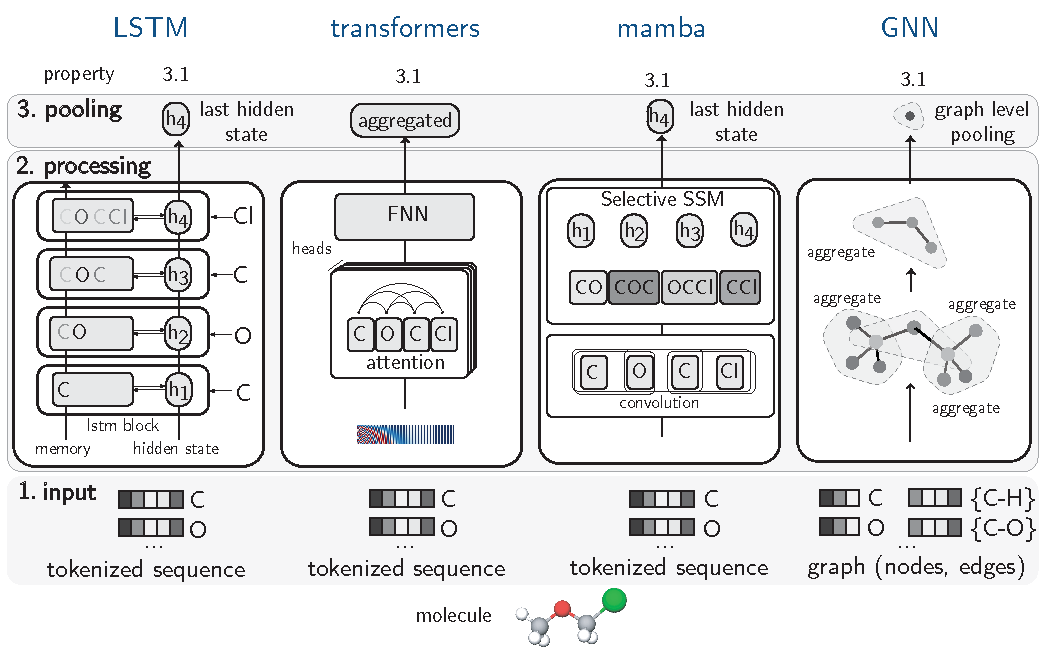
\includegraphics[width=1\textwidth]{figures/rescaled_figures/chemrev_figure6.pdf}
    \caption{\textbf{Blueprint for \glspl{gpm} architectures}. This diagram illustrates four distinct neural network architectures (\gls{lstm}, Transformer, Mamba, and \gls{gnn}), highlighting their unique approaches to input representation, information processing, and output pooling. \glspl{lstm} sequentially process tokens, accumulating information in a final hidden state with an inductive bias towards order. Transformers, conversely, use multi-head attention and positional encodings to capture global interactions simultaneously, offering minimal inductive bias but enabling rich contextual understanding. Mamba combines local convolutional processing with selective state space modeling to efficiently focus on chemically relevant parts, also typically using a final hidden state. \glspl{gnn} leverage the inherent graph structure of molecules, where atoms are nodes and bonds are edges, to model local chemical environments through message passing, followed by graph-level pooling to create a unified representation. Each approach offers unique strengths in how it captures molecular features, ranging from sequential to global, and graph-based relationships.}
    \label{fig:architectures}
\end{figure}


\paragraph{\gls{lstm}}

\gls{lstm} networks \autocite{hochreiter1997long} are well-suited for processing sequential data, such as text or time series. 
\Cref{fig:architectures} illustrates how chemical information is processed to predict \glspl{lstm}.
\begin{itemize}
    \item \textbf{Input}: Molecules are represented as tokenized sequences (e.g., \gls{smiles} strings like \enquote{COCCl}), processed one token at a time. Each token corresponds to an atom.
    \item \textbf{Processing}: Information flows sequentially through \gls{lstm} blocks where each hidden state ($h_{1}$, $h_{2}$, $h_{3}$, $h_{4}$) accumulates information about the molecule. The memory cell maintains chemical context through gating mechanisms. The inductive bias is sequential processing---assuming chemical properties emerge from analyzing tokens in order.
    \item \textbf{Pooling}: The final hidden state ($h_{4}$) captures the entire molecular information after processing the complete sequence. This last state serves as the molecular representation for the downstream task.
\end{itemize}

\glspl{lstm} process information in a strict sequence.  For the model to connect the first word to the last, that information must pass through every single step in between. The cost of \enquote{talking} across the sequence grows with the sequence length. 
Furthermore, the entire history of the sequence must be compressed into a single, fixed-size hidden state.

An \gls{xlstm} overcomes this with two key changes. \gls{xlstm} uses enhanced gates (act like filters to control what information flows) to precisely revise its memory. Second, instead of a single memory bottleneck, it uses a parallel \enquote{matrix memory}. This provides multiple \enquote{slots} to store different pieces of information at the same time. This structure allows it to process information in parallel, making it much more efficient.
\modelname{Bio-xLSTM} adapts this architecture for biological and chemical sequences, demonstrating proficiency in generative tasks and in-context learning for DNA, proteins, and small molecules.\autocite{SchmidingerSSSH25}


\paragraph{Transformer}

Transformers \autocite{vaswani2017attention} are also designed for sequential data, but are particularly powerful in capturing long-range dependencies and rich contextual relationships within sequences. 
Their core \enquote{attention mechanism} allows them to weigh the importance of different parts of the input simultaneously (quadratic computational scaling---if you double the length of the sequence, the amount of work the model needs to do quadruples). 
Effectively, they can be thought of as a fully connected graph model,\autocite{velivckovic2023everything, joshi2025transformers} where each representation of a token is connected to every other token and can impact its representation.

\begin{itemize}
    \item \textbf{Input}: Similar to \glspl{lstm}, data is tokenized and often enhanced with positional encodings (see \Cref{fig:architectures}, the tokenized sequence is added with positional information, e.g., using a sinusoidal signal---the red-blue spectrum) to maintain information about where in a sequence a token is placed (the attention mechanism itself does not preserve this information).
    \item \textbf{Processing}:  Uses attention mechanisms, where every atom/token attends to every other token simultaneously. This enables the capture of long-range interactions between distant elements of the sequence, regardless of their sequential distance. The \gls{fnn} transforms these attention-weighted representations.  To get a more robust and comprehensive understanding of the relationships within a sequence, models don't just rely on a single way of \enquote{paying attention}.  Instead, they employ multiple independent \enquote{attention heads} known as multi-head attention.
    \item \textbf{Pooling}:  Uses an aggregated representation or special token that combines information from all tokens, enabling global molecular property prediction.
\end{itemize}

\paragraph{Mamba}
Mamba\autocite{gu2023mamba0} is designed to be highly efficient (linear computational scaling) and effective at modeling very long sequences, offering a potentially more scalable alternative to Transformers for certain sequential tasks (for example, modelling very long protein sequences or polymer chains, while retaining strong performance in capturing dependencies.

\begin{itemize}
    \item \textbf{Input}:  Sequences similar to \gls{lstm}.
    \item \textbf{Processing}:  First applies convolution to capture local contexts, creating representations that incorporate neighboring information. These contextualized tokens are then processed through a \gls{ssm}. An \gls{ssm} is a type of sequence model that efficiently captures and summarizes long-range dependencies by tracking an evolving internal \enquote{state} (evolving representation of all the relevant information) based on inputs. This \gls{ssm} dynamically focuses on relevant parts. The inductive bias combines local patterns (through convolution) with efficient selective attention for handling long-range dependencies.
    \item \textbf{Pooling}:  Uses the final hidden state ($h_{4}$) similar to \gls{lstm}, but this state contains selectively processed information that more efficiently captures important features.
\end{itemize}
This architectural approach has been successfully applied to chemical foundation models, demonstrating \gls{sota} results in tasks like molecular property prediction and generation while maintaining fast inference on a large dataset of \gls{smiles} samples.\autocite{soares2025mamba-based} 



\paragraph{\gls{gnn}}
\gls{gnn} is an architecture that complements graph representations (see the section discussing graph-based representation \Cref{sec:common_representations}). Molecules are represented as graphs, where atoms are nodes and bonds are edges. \glspl{gnn} operate on these graphs by processing node and edge representations. Based on how the nodes are connected through edges, the information in these representations is updated multiple times. This procedure is called message passing (see \Cref{fig:architectures}). Information from neighbors is aggregated, and this aggregation occurs for all nodes and sometimes also for edges.

\begin{itemize}
    \item \textbf{Input}: Graphs, which are collections of nodes (e.g., atoms) and edges (e.g., bonds).
    \item \textbf{Processing}: Uses message passing through multiple aggregation steps (message would be the information in node or edge at the current stage, and aggregation can be different types of operations like adding information, taking mean, etc, depending on the architecture choice). Each node updates its representation based on messages from its bonded neighbors. The inductive bias is the graph structure itself, which naturally aligns with chemical bonding patterns.
    \item \textbf{Pooling}: Graph-level pooling (e.g., taking the mean of all node representations) aggregates information from all atoms and bonds to create a unified molecular representation, respecting the molecular graph structure.
\end{itemize}

\noindent These architectures cannot solve all problems equally well because they are tailored to different data structures. 
\gls{lstm} and Mamba inherently excel at processing sequential data; Transformers need to learn the structure, Transformers are powerful at capturing global relationships across the entire input,
whereas \glspl{gnn} are designed for graph-structured information. 
Forcing one type to handle data optimally it was not intended for, often leads to suboptimal performance, inefficiency, or requires extensive, task-specific adaptations that dilute its \enquote{general-purpose} nature.\autocite{alampara2024mattext}


\subsection{Multimodality}

Multimodal capabilities enable systems to process and understand multiple types of data simultaneously. 
Unlike traditional unimodal models, which work with a single data type (e.g., text-only or image-only), multimodal models can integrate and reason across different modalities, such as text, images, molecular structures, and spectroscopic data.

The core principle behind multimodal models lies in learning shared representations across different data types.  The challenge of creating this shared representation can be addressed through several architectural strategies, each with a different approach to learning the joint distribution of multimodal data. One dominant strategy is joint embedding alignment, where separate, specialized encoders are used for each modality (e.g., a \gls{gnn} for molecular structures and a Transformer for text). These encoders independently map their respective inputs into their own high-dimensional vector spaces. The key learning objective, often driven by contrastive learning (see \Cref{sec:contrastive_learning}), is to align these separate spaces. 


Another common approach is input-level fusion, where different data types are tokenized into a common format and fed into a single, unified architecture. 
For instance, a molecular structure might be converted into a \gls{smiles} string, an image into a sequence of patches, and text into its standard tokens. These disparate token sequences are then concatenated and processed by a single large model, typically a Transformer. 
This architecture allows the model's attention mechanism to learn correlations between modalities at a fundamental level directly---an image patch can \enquote{attend} to a word in the description, for instance. 
A more recent and highly efficient variant is adapter-based integration, where a powerful, pre-trained unimodal model (models that take a single type of representation) (like an \gls{llm}) is frozen, and a small \enquote{adapter network} (see discussion about adapter in \Cref{sec:model_adaptation}) is trained to project the embeddings from a secondary modality (e.g., a molecule) into the \gls{llm}'s existing latent space. 
This adapter effectively learns to translate the new data type into the \gls{llm}'s native \enquote{language}, leveraging the \gls{llm}'s vast pre-existing knowledge without the need for complete re-training. 
For instance, a model might learn that the textual description \enquote{benzene ring} corresponds to a specific visual pattern in molecular diagrams and produces characteristic peaks in \gls{nmr} spectroscopy. 
This cross-modal understanding enables more comprehensive and contextually rich analysis than any single modality alone could provide.

\subsubsection{Multimodal Integration in Chemistry}\label{sec:multimodal_chem}

A molecule’s \gls{smiles} string alone might not reveal its 3-D conformational preferences. 
A spectrum alone could suggest many different molecular structures. 
However, coupling these modalities with textual knowledge (e.g., \enquote{the sample was prepared by X method}) could narrow down possibilities. 
Multimodal models have the potential to emulate a human expert who simultaneously considers spectral patterns, chemical rules, and prior knowledge to deduce a structure. 
Another motivation is to create generalist \gls{ai} models. 
Instead of having multiple independent models---one for spectral analysis, another for molecule property prediction, and another for text mining---a single model could handle diverse tasks by understanding multiple data types.
In this way, a researcher can ask a question in natural language, provide a molecule (in the form of a structure file or image) as context, and receive a helpful answer that leverages both structural and textual knowledge.

\modelname{MolT5} \autocite{edwards2022translation} adapted the \modelname{T5} transformer for chemical language by training on scientific text and \gls{smiles} strings, using a masking objective to reconstruct masked segments. 
This approach treats \gls{smiles} as a \enquote{language}, enabling \modelname{MolT5}  to generate both valid molecules and fluent text. 
Similarly, \modelname{Galactica} \autocite{taylor2022galactica}, an \gls{llm}, also incorporated \gls{smiles} into its training. Later, the \modelname{MolXPT}\autocite{liu2023molxpt0} model used \enquote{paired} examples (\gls{smiles} and textual description) by replacing chemical names in scientific texts with their corresponding \gls{smiles} strings and description. 
This pre-training approach enables \modelname{MolXPT} to learn the context of molecules within text and achieve zero-shot text-to-molecule generation (see \Cref{sec:mol_generation} for more details on this application).

Contrastive learning emerged as an alternative, aligning separate text and molecule encoders in a shared embedding space. 
The principle of learning here is the same as that explained in \Cref{{sec:contrastive_learning}}. \modelname{MoleculeSTM} \autocite{Liu2023multi0modal} aligns separate text and molecule encoders in a shared space using paired data. 
This dual-encoder approach enables tasks such as retrieving molecules from text queries and shows strong zero-shot generalization for chemical concepts.  
Another notable study is \modelname{CLOOME} \autocite{sanchez2023cloome}, which used contrastive learning to embed bioimaging data (microscopy images of cell assays) and chemical structures of small molecules into a shared space. 
Multimodal learning also enables the determination of molecular structure from spectroscopic data. 
Models trained on large datasets of simulated spectra \autocite{alberts2024unraveling}, which combine multiple spectral inputs, could accurately translate spectra into molecular structures. \autocite{chacko2024spectro,mirza2024elucidating}


Beyond just prediction, some multimodal models aim for cross-modal generation, creating one type of data from another (e.g., generating an \gls{ir} spectrum from a molecular structure). \textcite{takeda2023multi} developed a multimodal foundation model for materials design, integrating \gls{selfies} strings, \gls{dft} properties, and optical absorption spectra. 
Their approach involves encoding each type of data separately into a shared, compressed representation space. 
Then, a network learns to combine these compressed representations to understand the connections between them. 
This pre-training on a big dataset of samples enables both combined representations (joint embeddings summarizing all modalities) and cross-modal generation, allowing tasks like predicting a spectrum from a molecule or generating a molecule from desired properties, effectively learning the relationships between structure, spectra, and quantum properties.

Their approach involves encoding each type of data (like molecular structure or properties) separately into a shared, compressed representation. 
Then, a network learns to combine these compressed representations to understand the connections between them. 

A more recent approach is the integration of molecular encoders with pre-trained \glspl{llm}. 
Models like \modelname{InstructMol} \autocite{cao2023instructmol0} and \modelname{ChemVLM} \autocite{li2024seeing} use an \enquote{adapter} (see discussion about \modelname{LoRa} in \Cref{sec:model_adaptation}) to project molecular information into the \gls{llm}'s existing knowledge space. 
This two-stage process first projects molecule representations into the \gls{llm}'s token space through pre-training on molecule-description pairs. 
Subsequently, instruction tuning on diverse chemistry tasks (e.g., \gls{qa}, reaction reasoning) enables the \gls{llm} to leverage molecular inputs, significantly enhancing its performance on chemistry-specific problems.


The latest generation of foundation models is often natively multimodal, designed from the ground up to process text, images, and other data types seamlessly. 
Natively multimodal systems are characterized by a single, unified neural network trained end-to-end on a diverse range of data modalities. 
This approach contrasts with previous methods that would stitch together separate models for each data type, enabling a more seamless and nuanced understanding of context and relationships across different informational forms. 
In the scientific domain, natively multimodal systems are still being explored. However, evaluations suggest that these models are not yet robust for solving complex scientific research tasks.\autocite{alampara2024probing}


\subsection{Optimizations}

As \glspl{gpm} continue to grow in size and complexity, optimization techniques become critical for making these models practically deployable while maintaining their accuracy. 
This section discusses three key optimization approaches that have particular promise for chemistry foundation models: \gls{moe} architectures for efficient scaling, quantization, and mixed precision for memory and computational efficiency, and knowledge distillation for creating specialized, lightweight models.


\subsubsection{Mixture-of-Experts} \label{sec:arch-moes}
\gls{moe} is a neural network architecture that uses multiple specialized \enquote{expert} networks instead of one single, monolithic model. The core idea is to divide the vast problem space---the embedding space of all possible inputs---into more manageable, homogeneous regions. A region is considered \enquote{homogeneous} not because all inputs within it are identical, but because they share similar characteristics and can be processed using a consistent set of rules. For instance, in a chemistry model, one expert might specialize in organic molecules, while another focuses on inorganic crystals; each expert sees a more consistent, or homogeneous, set of problems. This division of labor is managed by a gating network, which acts like a smart dispatcher. This gating network is itself a small neural network, often referred to as a trainable router, because it learns during training how best to route the data to the most appropriate expert, thereby improving its decisions over time.
\gls{moe} models achieve efficiency through selectively activating only the specific experts needed for a given task, rather than activating the entire neural network for every task. Modern transformer models using \gls{moe} layers can scale to billions of parameters while maintaining manageable computational costs, as demonstrated by models like \modelname{Mixtral-8x7B}, which uses eight experts with sparsity.

\textcite{shazeer2017outrageously} demonstrated that using a sparsely-gated \gls{moe} layer can expand a network’s capacity (by over 1000 times) with only minor increases in computation. In this architecture, each expert is typically a \gls{fnn}, and a trainable router determines which tokens are sent to which experts, allowing only a subset of the total parameters to be active for any given input. 
 
An \gls{llm} for science with \gls{moe} architecture (\modelname{SciDFM} \autocite{sun2024scidfm}) shows that the results of expert selection vary with data from different disciplines, i.e., activating distinct experts for chemistry vs.\ other disciplines. They consist of multiple \enquote{expert} subnetworks, each potentially specializing in different facets of chemical knowledge or types of chemical tasks. A routing mechanism directs inputs to the most relevant expert(s). This allows the foundation model to be more adaptable and perform across the broad chemical landscape.  The \gls{moe} concept has also been adapted for physical simulations. The \modelname{UMA} family employs a \gls{moe} architecture with linear experts to build accurate yet computationally efficient interatomic potentials \autocite{wood2025uma0}. This approach builds route based on  global system properties (e.g., elemental composition, charge, spin) rather than per-token.


Extending this concept, a recent multi-view \gls{moe} model (\modelname{Mol-MVMoE} \autocite{shirasuna2024multi}) treats entire, distinct chemical models as individual \enquote{experts}. Rather than routing tokens within one large model, a gating network learns to create a combined molecular representation by dynamically weighting the embeddings from each expert model. This method showed strong performance on \modelname{MoleculeNet}, a widely used benchmark suite for molecular property prediction, outperforming competitors on 9 of 11 tasks.


Training \gls{moe} models can be a complex process. The gating mechanism must be carefully learned to balance expert usage and instability, or some experts may end up underutilized (most of the data would be processed by a subset of networks). \autocite {fedus2022switch} For chemistry tasks, an additional challenge is to ensure that each expert has access to sufficient relevant chemical data to specialize. If the data is sparse, some experts may not learn meaningful functions. Despite these hurdles, \glspl{moe} remain a promising optimization strategy to handle the breadth of chemical space.



\subsubsection{Quantization and Mixed Precision}
\label{sec:quantization}
Quantization is a technique for making models more computationally efficient by reducing their numerical precision. 
In experimental science, precision often relates to the number of significant figures in a measurement; a highly precise value, such as $3.14159$, carries more information than a rounded one, like $3.14$. 
Similarly, a model's knowledge is stored in its weights, which are organized into large matrices of numbers. Standard models typically use high-precision formats, such as 32-bit floating-point, which can represent a wide range of numbers with many decimal places to store weights. During inference, these weight matrices are multiplied by the input data to produce a prediction. Quantization involves converting these numbers into a lower-precision format, such as 8-bit integers, which are whole numbers with a much smaller range. This process is similar to rounding down your experimental data---it simplifies the numbers, uses less memory, and allows calculations to run much faster.

 
\textcite{dettmers2022gpt3} introduced an 8-bit inference approach (\texttt{LLM.int8}) enabling models as large as \modelname{GPT-3} (175B parameters) to run with no loss in predictive performance (less than $50\%$ GPU-memory usage).  
A key insight in this paper is that while most numbers in a model can be safely rounded, a few \enquote{outlier} values with large magnitudes are critical for performance. 

A different, yet related, strategy is mixed-precision quantization.\autocite{micikevicius2017mixed} Instead of applying a single precision format (like 8-bit) across the entire model, this approach uses a mix of different precisions for different parts of the network. The guiding principle is that some layers of the model might be more sensitive to rounding errors than others.


Many chemistry applications, particularly in automated laboratory setups, require deployment on edge devices---local computing hardware, such as the controllers for robotic arms or the onboard computers in analytical instruments---or cloud platforms with limited computational resources. Quantization can be a valuable optimization tool for reducing computational burden while increasing inference speed, which is crucial for real-time applications.


\subsubsection{Parameter-Efficient Tuning}
\label{sec:peft}

While full fine-tuning is computationally expensive, memory-intensive, and results in a complete, multi-gigabyte copy of the model for every new task. 
\gls{peft} methods offer a solution to this problem by freezing the vast majority of the trained model's weights and only training a very small number of new parameters. This is conceptually similar to attaching a small, specialized probe to a large, complex analytical instrument; you adapt its function for a new task without re-engineering the entire machine.

A prominent and widely used \gls{peft} technique is \gls{lora}.\autocite{hu2022lora}  
The key insight of \gls{lora} is that the change needed to adapt a pre-trained weight matrix for a new task can be approximated effectively using much smaller matrices. \gls{lora} freezes the original model weights and introduces small trainable rank-decomposition matrices into each transformer layer, significantly reducing the number of trainable parameters. 
Because these new matrices contain far fewer parameters—often less than 0.1\% of the original model—the computational and memory requirements for training are drastically reduced.
 
These optimization strategies can be combined with quantization (see \Cref{sec:quantization}) for even greater efficiency. \textcite{dettmers2023qlora} introduced \gls{qlora}. In this approach, the large pre-trained model is first quantized down to a very low precision (typically 4-bit), dramatically shrinking its memory footprint. 
Then, the lightweight \gls{lora} adapters are added and fine-tuned. The impact of this is profound: \gls{qlora} enables the fine-tuning of massive models---such as a 70-billion-parameter model---on a single, consumer-grade GPU.


\subsubsection{Distillation}

Knowledge distillation is a technique that aims to transfer the learning of a large pre-trained model (the \enquote{teacher model}) to a smaller \enquote{student model}. \autocite{hinton2015distilling}
The computationally more efficient \enquote{student model} is trained to mimic the behavior (e.g., output probabilities or internal representations) of the larger teacher model. 
This allows the rich, nuanced understanding learned by the large foundation model to be compressed into a more compact and faster student model.\autocite{sanh2019distilbert}

For example, recent work introduced a method for transferring general-purpose representations from machine learning force field (\gls{mlip}) foundation models to smaller, faster \glspl{mlip} specialized to specific regions of chemical space. Formulating the approach as a knowledge distillation procedure where the student \gls{mlip} is trained to match the Hessians of the energy predictions of the teacher foundation model. \autocite{amin2025towards}
Their specialized \glspl{mlip} achieved up to 20 times faster inference than the original foundation model while retaining, and in some cases exceeding, its performance.


Effective distillation requires that the teacher model is both competent at the task and that its knowledge is representable by the student. 
If the teacher is too large or complex compared to the student, the student may struggle to emulate it, leading to degraded performance. \autocite{liu2024wisdom}



\subsection{Model Level Adaptation}
\label{sec:model_adaptation}
Although promising, \glspl{gpm} such as \glspl{llm} rarely work straight out of the box for specialized tasks and often need customization. This is especially true for complex scientific problems where data is a limiting factor. 
By simply prompting an \gls{llm}---for example, by asking a question or giving instructions---one can observe that these models perform much better on general tasks than on those related to chemistry. 
This difference arises because \glspl{llm} are not typically trained on domain-specific chemical tasks and therefore they lack the necessary knowledge and reasoning skills. 

To bridge this gap, two complementary families of approaches exist. First approach involves adapting the model's knowledge or behavior directly. The simplest method is to embed information directly in the prompt, for instance by providing examples (\gls{icl}) \autocite{brown2020language} or by introducing intermediate reasoning steps (\gls{cot}) \autocite{wei2022chain}. However, not all problems can be solved in these ways, and sometimes it is necessary to tune the model to new data which updates its parameters. 
The second approach involves coupling the model into a larger system that can interact with external sources of information and tools.


\begin{table}[!ht]
    \centering
    \caption{\textbf{Model Adaptation Approaches Overview:} This table provides a rough overview of the estimated time, data, and \gls{ml} knowledge required for each approach. Each method (listed in the first column) is paired with a triplet that includes: an approximate implementation time, the estimated dataset size, and the level of \gls{ml} expertise needed.  These estimates assume that you have at least a bachelor's level of understanding of chemistry and at least some computational background.}
\begin{tabular}{llll}
\toprule
    \textbf{Model adaptation}  & \textbf{Time}    & \textbf{Data}   & \textbf{ML knowledge}  \\ 
\midrule
Pre-training       & Weeks   & 1M--1B+      & Very High  \\
Zero-shot prompting & Minutes & None        & None          \\
Few-shot Prompting   & Hours   & \textless 10 examples & None          \\
Fine-tuning         & Days    & \textless 10k         & High          \\
\toprule
    \textbf{Coupling into systems} \\ 
\midrule
RAG                & Days    & 100k--1M+    & Low           \\
Tool-Augmentation   & Days    & None / 10k+ & Low           \\
\bottomrule
\end{tabular}
    \label{tab:model_adaptation}
\end{table}




\paragraph{Prompting}\label{sec:prompting} \glspl{llm} have demonstrated the ability to perform a wide range of tasks based solely on prompt instructions---without the need for fine-tuning \autocite{radford2019language}. 
This ability, for \glspl{llm} to complete tasks without any additional information is often referred to as zero-shot prompting.
By providing task-specific examples directly within the input prompt, \glspl{llm} can draw analogies and generalize to new tasks, a capability known as \gls{icl} \autocite{brown2020language, chowdhery2023palm, openai2023gpt04}. 
In \gls{icl}, the model is presented with a few demonstration examples alongside a query, all within the same input—--a technique known as few-shot prompting. 
The model's parameters remain unchanged; instead, it is expected that the model can recognize patterns within the prompt and generate an appropriate response \cite{von2023transformers}. \gls{icl} enables models to learn on the fly, reducing the barrier to entry for users without deep \gls{ml} expertise. 
However, because the model does not retain memory between queries, the learned knowledge is temporary and is subsequently lost in subsequent queries. 
Additionally, \gls{icl} tends to struggle with tasks that require multi-step reasoning \autocite{brown2020language}. 
To address this limitation, task decomposition techniques have been introduced, with the earliest being \gls{cot} \autocite{wei2022chain}. 
Rather than relying solely on examples, this approach enriches the prompt with a series of reasoning steps that guide the model toward the correct answer \autocite{wei2022chain}. 
Considering that prompting approaches do not require an in-depth understanding of machine learning, they have proven very useful for a range of chemical tasks, including chemical data extraction, \gls{qa}, and property prediction \autocite{liu2025integrating, zheng2023chatgpt, mirza2024large}.


\paragraph{Fine-tuning} \label{sec:fine-tuning} 
What separates fine-tuning from the other approaches discussed is that it directly changes the weights of the model as well as its broad applicability across different model architectures, not just \glspl{llm}. 
Apart from changing the weights (see \Cref{sec:fine_tuning_coloring}), unlike techniques like \gls{icl} or prompt engineering that are limited to \glspl{llm}, fine-tuning can be applied to a wide variety of architectures, including other transformer-based models, \glspl{gnn}, \glspl{cnn}, and others. 
The fine-tuning strategy depends on the size and complexity of the target dataset as well as the pre-trained model. For many tasks, especially when using a powerful pre-trained model, it is often sufficient to freeze the entire model except for the final layer and only train that layer's parameters. 
However, as the target task diverges more significantly from the pre-trained model’s original objectives, more adaptation may be necessary. This can include replacing specific layers in the model to better suit the new task. For instance, in autoencoder architectures, it's common to freeze the encoder and replace the decoder. In \glspl{gnn}, the graph convolutional layers are typically frozen, while the final fully connected layers are replaced and re-trained. In some cases, it may be necessary to fine-tune the entire model, an especially resource-intensive process for \glspl{llm}, whose parameters can be in billions. To speed up this process, methods like \gls{peft} have been developed (see more details in \Cref{sec:peft}). 
Despite these innovations, one key limitation of fine-tuning remains: adapting to a new modality, which often requires architectural changes or switching to a different model. However, \glspl{llm} offer a unique workaround. Many regression or classification tasks can be reformulated into a text-based format, allowing a single language model to be fine-tuned across a wide range of tasks. This is known as \gls{lift} \autocite{dinh2022lift}, which enables us to utilize a single \gls{gpm} for a diverse set of tasks.

Beyond adapting a model's internal knowledge through prompting or fine-tuning, its capabilities can be  expanded by coupling it with external resources. This approach transforms a static model into a dynamic problem-solver that can access up-to-date information and perform actions in the world. This practice of designing and delivering task-relevant information is often referred to as context engineering. The necessary context can be provided through several complementary approaches that operate during inference time. This is achieved by coupling \gls{llm} into a system of resources.

\subsection{System-level Integration: Agents} \label{sec:agents}

While powerful, \glspl{gpm} are fundamentally static entities. Their knowledge is frozen at the time of training, and they lack the ability to interact with the world beyond the information they process.  They cannot browse the web for the latest research, execute code to perform a calculation, or control a robot to run an experiment. 
To overcome these limitations and apply the reasoning capabilities of \glspl{gpm} to complex, multistep scientific problems, so-called \gls{llm}-based agents have emerged.

An \gls{llm}-based agent is a system that leverages an \glspl{llm} as its core \enquote{brain} but couples it with a set of tools to perceive and act upon its environment. To use a tool, the agent simply generates text containing the tool's name and its required inputs (arguments). The framework managing the agent recognizes this specific text, executes the corresponding tool, and then feeds the result back to the \gls{llm}. This transforms the model from a passive generator of text into an active problem-solver that can formulate plans, execute actions, observe the results, and adapt its strategy accordingly.  For chemists and material scientists, this paradigm shift is profound. It moves from asking a model a question to giving it a research goal, which it can then pursue autonomously.

\Cref{fig:agent-loop} illustrates the fundamental components of an agentic framework, often conceptualized through the interacting modules of perception, cognition, and execution. It is important to note that this is one possible way to formalize an agent's architecture; other organizational structures exist. Rather than a strict, sequential loop, these components represent a set of capabilities that the agent's core \gls{llm} can dynamically draw upon to achieve complex objectives.

\begin{figure}[htb]
    \centering
    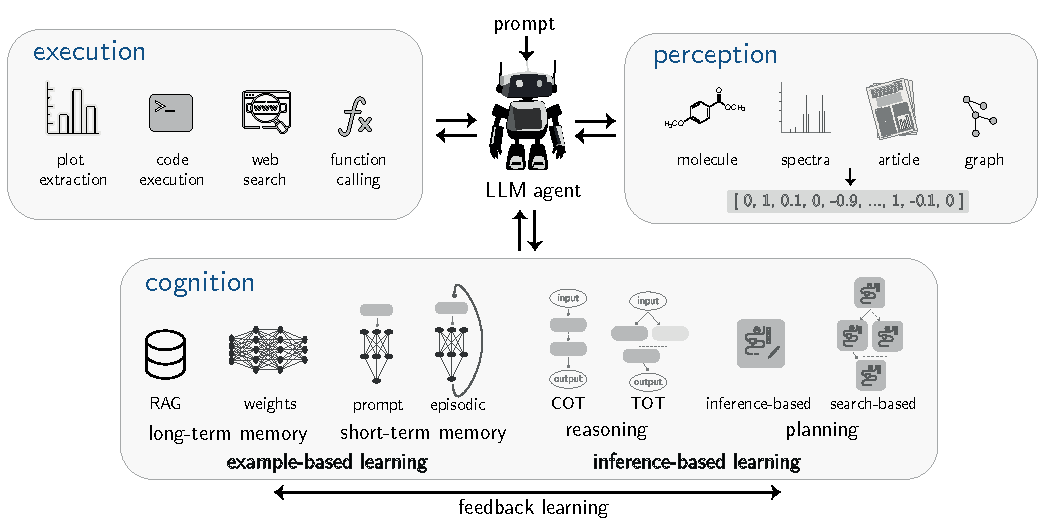
\includegraphics[width=1\textwidth]{figures/rescaled_figures/chemrev_figure7.pdf}
    \caption{\textbf{The execution-cognition-perception capabilities of an \gls{llm}-agent:} This figure illustrates how agents orchestrate complex problems. At the core, an \gls{llm}-agent coordinates multiple capabilities. Upon prompting, the agent can execute tools. Tools include but are not limited to running code, searching for information, or calling functions. These actions feed into the agent's perception system, which transforms raw data into structured representations (in combination, for example, agents can obtain figures' information by executing \gls{ocr} tools on paper). The cognitive architecture underneath serves as the \enquote{agent's brain}, utilizing both memory systems (long-term knowledge storage and short-term contextual awareness) alongside reasoning mechanisms and planning strategies. This creates a dynamic setup, where execution produces observations, cognition interprets those observations and formulates plans, and new actions are taken based on improved understanding.}
    \label{fig:agent-loop}
\end{figure}

\subsubsection{Core Components of an Agentic System}\label{sec:arch_agents}

An agent is a system composed of several key components that work in concert.

\paragraph{Cognitive Engine} This is typically a powerful \gls{llm}. It is responsible for all high-level reasoning, including understanding the user's objective, breaking it down into smaller, manageable steps (see planning \Cref{sec:planning}), and deciding which tools to use to accomplish each step.

\paragraph{Tool Augmentations (Execution)}
\label{sec:tool_augmentation}
Tools are external programs or functions that the agent can call upon to perform actions. They allow agents to interact with the world beyond their internal knowledge. \autocite{schick2023toolformer, parisi2022talm}. Tool augmentation can range from simple tools, such as calculators, to more complex systems that involve web searches, code execution, and integration with robots \autocite{darvish2025organa, chan2024mle, wei2025browsecomp}. In a chemical context, tools can be as simple as a stoichiometry calculator or as complex as a Python script that runs a \gls{dft} simulation using specialized software, a search \gls{api} for querying chemical databases like \modelname{PubChem}, or a controller for a robotic synthesis platform \autocite{boiko2023autonomous, darvish2025organa, bran2024augmenting}.

\paragraph{Memory \& \gls{rag} }
\label{sec:rag}
Agents need to maintain context over long and complex tasks. The memory module provides this capability. Short-term memory is often handled within the finite context window (i.e., number of tokens an \gls{llm} can process), keeping track of the immediate chain of thought and recent actions.
While short-term memory (e.g., context) is transient, \glspl{llm}'s model weights serve as long-term memory. However, these weights often lead to reduced performance on knowledge-intensive scientific tasks and increased susceptibility to hallucinations---generating incorrect or fabricated information \autocite{marcus2020next}.
One effective way to address this limitation is to pair the model with an external knowledge base.\autocite{lewis2020retrieval} Such Long-term memory can be implemented using external databases (e.g., vector stores) where the agent can store and retrieve key findings, successful strategies, or experimental results from past interactions, enabling it to learn and improve over time \autocite{chen2023chemist}. The widely adopted execution of Long-term memory is \gls{rag}. \gls{rag} works by retrieving a set of relevant documents from a designated knowledge database based on the input query. These retrieved documents are then concatenated with the original prompt and passed to the \gls{llm}, which generates the final output.  In scientific applications, this is particularly valuable, as the system can be continuously updated with the latest research and discoveries. In the field of chemistry, \gls{rag} has primarily been used to answer domain-specific questions based on scientific literature and assist in experimental design \autocite{chen2023chemist, skarlinski2024language}.


\subsubsection{Approaches for building Agentic System}

A well-known approach for building \gls{llm}-based agents is called \gls{react}\autocite{yao2023react}. In \gls{react}, the agent repeatedly goes through a cycle of thinking, performing an action, and then reasoning about the tool output. 
This structured problem-solving is achieved by prompting the model to generate its response following a specific \enquote{Think}, \enquote{Act}, \enquote{Observe} format.
First, the agent considers the problem it needs to solve, focusing on its primary objective. It devises a plan, identifies any missing information, and determines which tool can help it move forward. Next, the agent acts by selecting and utilizing the appropriate tool with the necessary information. For instance, if it needs to find a compound's boiling point, it might use a tool that searches a chemical database using the compound's name or its \gls{smiles} string. After that, the agent observes the outcome by examining the tool's output. This output then becomes new information for the agent. The agent then repeats the cycle, taking this new observation into account as it plans its following action. This loop continues until the agent reaches its main goal. This repeating process helps the agent deal with mistakes, adjust to unexpected results, and break down a big task, like \enquote{finding a better catalyst for this reaction}, into smaller, manageable steps that involve using tools.

While a single agent can effectively tackle linear problems---tasks that can be solved through a predictable sequence of steps---complex scientific discovery often requires diverse expertise and collaborative problem-solving. This has led to the development of multi-agent systems, which move beyond a single cognitive engine to orchestrate a team of agents that work together \autocite{wu2023autogen}. These systems can solve tasks that are too complex or multifaceted for any single agent to handle alone by enabling agents to communicate, delegate, and debate. \autocite{lazaridou2020emergent}
Several collaborative paradigms have emerged, each offering unique advantages:

\paragraph{Specialization and Division of Labor} \label{sec:multi-agent}
Just as a human research group has members with different roles, multi-agent systems can be composed of specialized agents. For example, in a chemistry context, a \enquote{Planner} agent might design a high-level research plan, a \enquote{Literature Searcher} agent could retrieve relevant papers, a \enquote{Computational Chemist} agent could run \gls{dft} simulations, and a \enquote{Safety Expert} agent could check proposed reaction steps for hazards.\autocite{Zou2025ElAgente} This division of labor shows this role-playing approach to be highly effective for complex tasks like software development, where agents take on roles such as \enquote{programmer}, \enquote{tester}, and \enquote{documenter} \autocite{qian2024chatdevcommunicativeagentssoftware}.

\paragraph{Refinement of Answers} A key weakness of single \glspl{llm} is their tendency to hallucinate or pursue a flawed line of reasoning. Multi-agent systems can mitigate this by introducing criticism and debate. In this paradigm, one agent might propose a solution (e.g., a synthetic pathway), while a \enquote{Critic} agent is tasked with finding flaws in the proposal. This adversarial or collaborative process forces the system to refine its ideas, correct errors, and explore alternatives, leading to more robust and reliable outcomes \autocite{liang2024encouragingdivergentthinkinglarge, du2023improving}. 

\paragraph{Context Compression through Parallelism}
A significant operational challenge for any \gls{llm}-based system is the finite context window. 
As a task becomes more complex, the conversational history can grow cluttered with irrelevant details, degrading the model's performance.\autocite{chirkova2025provence0, lee2024long1context} 
Multi-agent systems offer a powerful solution to this problem through a strategy that can be described as context compression. 
By assigning sub-tasks to specialized agents, the system allows each agent to operate in parallel with its own clean, dedicated context window. 
For example, a \enquote{Literature Searcher} agent's context is filled only with search queries and retrieved text, while a \enquote{Computational Chemist} agent's context contains only simulation inputs and results. 
These sub-agents essentially act as filters; they process large amounts of information and then \enquote{compress} their findings into concise summaries or structured data. 
These distilled insights are then passed back to a lead agent or aggregated. 
This not only dramatically speeds up information gathering but also ensures that the primary reasoning process is not diluted by excessive or irrelevant information, leading to higher quality and more reliable outcomes \autocite{Breunig2025HowToFixYourContext}.


\paragraph{Swarm Intelligence and Parallel Exploration}
Inspired by natural systems like ant colonies, some multi-agent approaches use a \enquote{swarm} of less-specialized agents to explore a vast problem space in parallel. Instead of assigning fixed roles, a multitude of agents can independently investigate different hypotheses or search different regions of a chemical space. Their collective findings can then be aggregated to identify the most promising solutions. This is particularly powerful for optimization and discovery tasks, such as high-throughput virtual screening or materials design, where the goal is to efficiently search an enormous number of possibilities \autocite{chen2023agentversefacilitatingmultiagentcollaboration}.


It is also crucial to distinguish between the foundational model itself (e.g., the GPT-4 \gls{llm}) and the \enquote{system} with which the user interacts (e.g., ChatGPT). Such systems are not merely the raw model; they incorporate additional layers for safety, prompt management, and some of the adaptation techniques discussed in this section. Understanding this distinction is key to understanding how a static model is transformed into a dynamic and useful tool.
\section{Evaluations} \label{sec:evals}
\subsection{The Evolution of Model Evaluation}

Assessing modern \glspl{gpm} is challenging due to their broad applicability across diverse domains. 
Unlike traditional models, which are designed for specific tasks and can be directly tested on well-defined objectives \autocite{raschka2018model}, it is impractical to evaluate \glspl{gpm} on every possible capability. As a result, many evaluations rely on structured benchmarks that measure proficiency in key areas such as mathematics, chemistry, and language understanding \autocite{tikhonov2023post}. 
However, such benchmarks often fall short in capturing open-ended problem-solving or emergent abilities that arise without explicit training for them and are sensitive to factors such as prompt phrasing and task framing \autocite{Siska2024}.

Early benchmarks primarily focused on evaluating specialized models based on their ability to predict molecular properties from molecular structures. \autocite{wu2018moleculenet} 
While useful, these evaluations largely emphasized numerical accuracy on the isolated tasks the models were fine-tuned on, without probing the more complex reasoning or generative capabilities that \glspl{gpm} aim to capture. 
Over time, this evolution expanded to exam-like problem-solving, assessing structured tasks similar to those found in academic chemistry courses. \autocite{zaki2023mascqa0, li2023camel} 
More recent efforts aim to evaluate a broader range of skills, including knowledge retrieval, logical reasoning, and even the ability to mimic human intuition when solving complex chemical problems.\autocite{feng2024sciknoweval0, mirza2024large} 
This shift highlights the need for more flexible evaluation methods that consider the specific context and nature of each task. Rather than relying solely on static benchmarks, there is a growing demand for assessments that dynamically account for the diversity of chemical tasks and the specific capabilities required to solve them---mirroring the multifaceted potential of \glspl{gpm} in chemistry. \Cref{tab:chemistry_benchmarks,fig:benchmarks} gives an overview of some benchmarks that have been used in the chemical sciences.


\begin{table}
\centering
\footnotesize
\caption{\textbf{Non-comprehensive overview of chemistry benchmarks}. Overview of chemistry benchmarks including the topics covered, the curation method (automated, using \glspl{llm}, manual), and the number of questions. We limit our scope here to benchmarks (and exclude other evaluation methods), since they constitute the most actively used and publicly available resources in the field at present.}
\label{tab:chemistry_benchmarks}
\begin{tabular}{p{3cm} p{6.9cm} p{1.2cm} p{1cm}}
\toprule
\textbf{Benchmark name} & \textbf{Overall topic} & \textbf{Curation method} & \textbf{Count} \\
\midrule
CAMEL - Chemistry \autocite{li2023camel} & General Chemistry \gls{mcq} & A, L & 20 K \\
ChemBench \autocite{mirza2024large} & General Chemistry \gls{mcq}, Reasoning & M & 2.7 K \\
ChemIQ \autocite{runcie2025assessing} & Molecule Naming, Reasoning, Reaction Generation, Spectrum Interpretation & A & 796 \\
ChemLLM \autocite{zhang2024chemllm} & Molecule Naming, Property Prediction, Reaction Prediction, Reaction Conditions Prediction, Molecule \& Reaction Generation, Molecule Description & A, L & 4.1 K \\
ChemLLMBench \autocite{guo2023large} & Molecule Naming, Property Prediction, Reaction Prediction, Reaction Conditions Prediction, Molecule \& Reaction Generation & A, L & 800 \\
LAB-Bench \autocite{laurent2024lab0bench0} & Information Extraction, Reasoning, Molecule \& Reaction Generation & A, M & 2.5 K \\
LabSafety Bench \autocite{zhou2024labsafety} & Lab Safety, Experimental Chemistry & M, L & 765 \\
LlaSMol \autocite{yu2024llasmol} & Molecule Naming, Property Prediction, Reaction Prediction, Reaction Conditions Prediction, Molecule \& Reaction Generation, Molecule Description & A, L & 3.3 M \\
MaCBench \autocite{alampara2024probing} & Multimodal Chemistry, Information Extraction, Experimental Chemistry, Material Properties \& Characterization & M & 1.2 K \\
MaScQA \autocite{zaki2023mascqa0} & Material Properties \& Characterization, Reasoning, Experimental Chemistry & A & 650 \\
MolLangBench \autocite{cai2025mollangbench} & Molecule Structure Understanding, Molecule Generation & A, M & 4 K\\
MolPuzzle \autocite{guocan} & Molecule Understanding, Spectrum Interpretation, Molecule construction & A, L, M & 23 K \\
SciAssess \autocite{cai2024sciassess0} & General Chemistry MCQ, Information Extraction, Reasoning & A, M & 2 K \\
SciKnowEval \autocite{feng2024sciknoweval0} & General Chemistry MCQ, Information Extraction, Reasoning, Lab Safety, Experimental Chemistry & A, L & 18.3 K \\
\bottomrule
\end{tabular}
\begin{tablenotes}
\footnotesize
\item \textbf{Abbreviations:} 
A: Automated methods, L: Usage of \glspl{llm}, M: Manual curation.
\end{tablenotes}
\end{table}


\begin{figure}
    \centering
    \label{fig:benchmarks}
    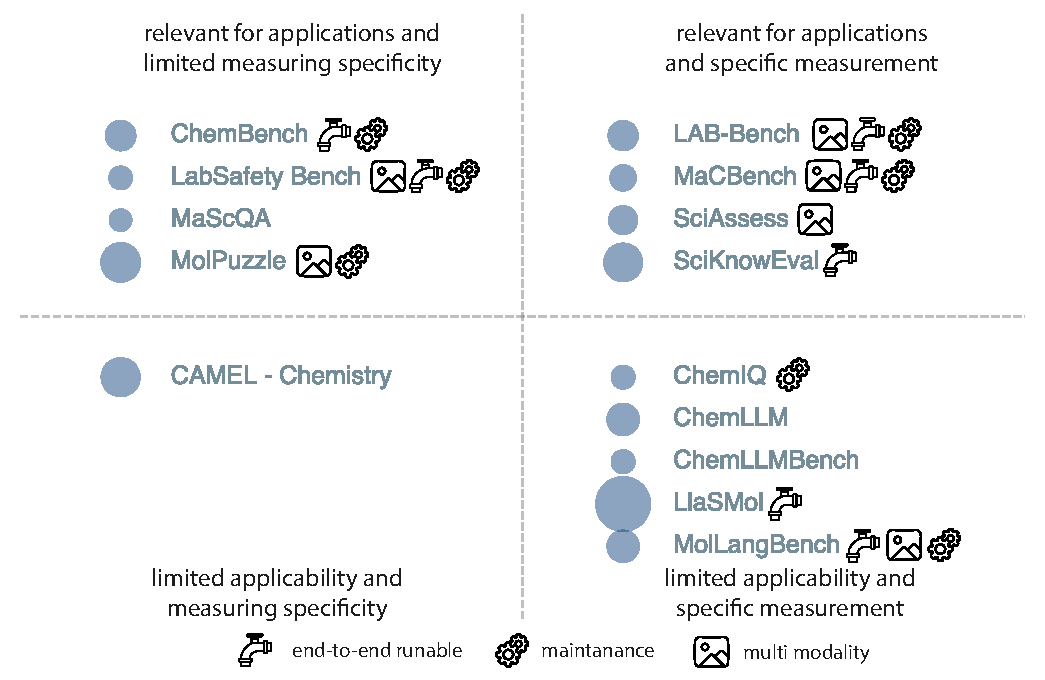
\includegraphics[width=1\textwidth]{figures/rescaled_figures/chemrev_figure8.pdf}
    \caption{\textbf{Comparison of measurement specificity and application relevance of chemistry benchmarks.} This figure presents a subjective, qualitative positioning of selected chemistry-related benchmarks along the axes of application relevance and measurement specificity (the extent to which a benchmark evaluates well-defined and objectively measurable outputs---such as physical or chemical properties---rather than more ambiguous tasks like answering general chemistry trivia or \gls{mcq}). The icons indicate whether a benchmark incorporates multimodal inputs (e.g., images or spectra), when it is actively maintained (based on GitHub activity within the past 6 months), and if it supports end-to-end evaluation via a clearly described pipeline with code provided by the authors.}
\end{figure}


\subsection{Design of Evaluations}
\label{sec:eval_design}

\paragraph{Desired Properties for Evaluations}
To meaningfully evaluate \glspl{gpm}, we must first consider what makes a good evaluation. 
Ideally, an evaluation should provide insights that translate into real-world impact, allowing comparisons between models. 
Thus, evaluation results must be stable over time and reproducible across different environments---assuming access to the same model weights or version, which is not always guaranteed when using proprietary \glspl{api}. \autocite{Ollion2024dangers}
A key challenge is so-called construct validity---ensuring that evaluations measure what truly matters rather than what is easiest to quantify. For example, asking a model to generate valid \gls{smiles} strings may test surface-level structure learning but fails to assess whether the model understands chemical reactivity or synthesis planning.
Many methods fall into the trap of assessing proxy tasks instead of meaningful competencies, which leads to misleading progress. 
However, it is important to note that proxy tasks are often chosen because measurements at higher fidelity are more expensive or time-consuming to construct. 


\paragraph{Data and Biases} The choice of what and how to measure is highly impacted by the data. 
Datasets in chemistry often differ in subtle but impactful ways: biases in chemical space coverage (e.g., overrepresented reaction types) \autocite{Jia_2019anthropogenic,Fujinuma_2022why}, variations in data fidelity (e.g., \gls{dft} vs. experimental measurements),  inconsistent underlying assumptions (e.g., simulation level or experimental conditions), and differences in task difficulty. 
These differences can distort what evaluations actually measure, making comparisons across models or tasks unreliable. \autocite{peng2024survey}
Moreover, the process of collecting or curating data itself introduces further variability, introduced by incomplete or biased coverage of the chemical space, computational constraints, or design decisions in the construction of tasks. 
As such, evaluations must be built using transparent, well-documented construction protocols, with clearly stated scope and limitations.


\paragraph{Scoring Mechanism} 

\begin{figure}
    \centering
    \label{fig:scoring}
    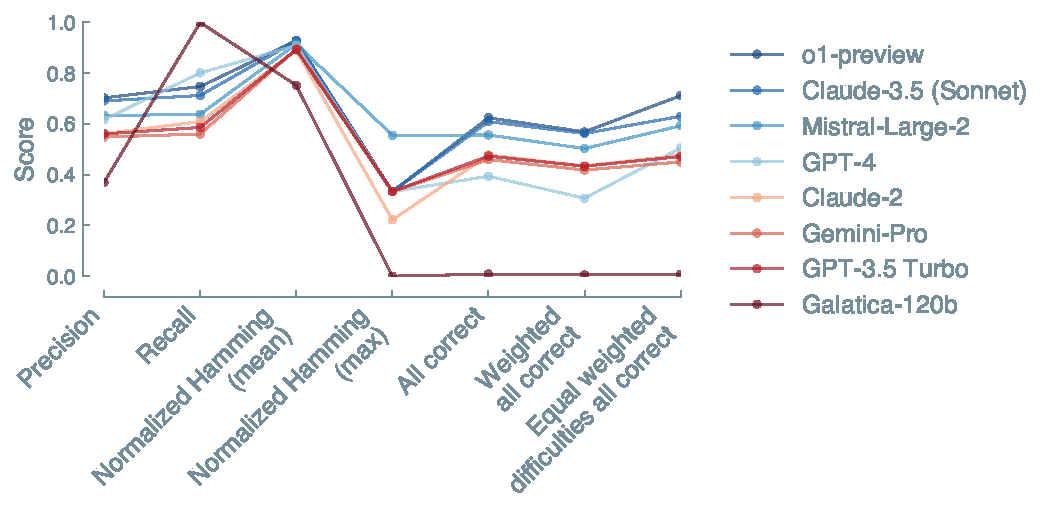
\includegraphics[width=1\textwidth]{figures/final_figures/chembench_scoring.pdf}
    \caption{\textbf{\modelname{ChemBench} \autocite{mirza2024large} rankings based on different scoring metrics}: All metrics are a sum, weighted sum, or maximum values over all \glspl{mcq}. The weighted sums are calculated by taking the manually rated difficulty (basic, immediate, advanced) of the question into account. For equal weighting, all categories are weighted equally, regardless of the number of questions. The metric \enquote{all correct} is a binary metric indicating if a given answer is completely correct. For normalized Hamming (max), the normalized maximum value of the Hamming loss of each model was taken. We find that the ranking of models changes if we change the metric, or even just the aggregation---showcasing the importance of proper and transparent evaluation design.}
\end{figure}

The way model performance is scored has a direct impact on how results are interpreted and compared. 
Leaderboards and summary statistics often shape which models are considered state-of-the-art, making even small design choices in scoring, such as metric selection, aggregation, or treatment of uncertainty, highly consequential (see \Cref{fig:scoring}). 
Inconsistent or poorly designed scoring can lead to misleading conclusions or unfair comparisons.
Metric selection and aggregation critically shape evaluation outcomes. 
For example, in tasks where multiple correct answers are possible different evaluation strategies yield different insights: a permissive metric may assign partial credit for each correct option selected, while a stricter \enquote{all-or-nothing} metric only gives credit if the full set of correct choices is identified without any mistakes. The former captures varying levels of performance, while the latter enforces a binary pass or fail threshold. Aggregation strategies, such as task averaging or difficulty-based weighting, further influence the overall score and can substantially shift model rankings. 

\paragraph{Statistical significance and uncertainty estimation} Statistical significance and uncertainty estimation are essential for drawing robust conclusions. Evaluations must include a sufficient number of questions per task type to ensure statistical power, and repeated runs (e.g., different seeds or sampling variations) are needed to report confidence intervals or error bars. \autocite{tikhonov2023post} 
While this is feasible for automated, large-scale benchmarks, it becomes significantly more challenging in resource-intensive settings such as real-world deployment studies (e.g., testing a model in a wet-lab setting), where replicability and scale are limited.

\paragraph{Reproducibility and Reporting} Without clear and consistent documentation, even well-designed evaluations risk being misunderstood or unreproducible. 
To ensure that results are interpretable, verifiable, and extensible, every step of the evaluation process should be clearly specified, from prompt formulation and data pre-processing to metric selection and aggregation. 
Standardized evaluation protocols, careful tracking of environmental variables (e.g., hardware, model version, and sampling settings such as the inference temperature for \glspl{llm}), and consistent version control (documenting the exact version of the used model) are essential to avoid unintentional variation across runs. 
Additionally, communicating limitations and design decisions openly can help the broader community understand the scope and reliability of the reported results. 
\textcite{alampara2025lessons} proposed evaluation cards as a structured format to transparently report all relevant details of an evaluation, including design choices, assumptions, and known limitations, making it easier for others to interpret, reproduce, and build upon the results.


\subsection{Evaluation Methodologies}
\label{sec:eval_methods}
\paragraph{Representational vs.\ Pragmatic Evaluations}
It is useful to think of evaluations in \gls{ml} as living on a spectrum from representational to pragmatic. 
Representational evaluations focus on measuring concepts that exist in the real world. For instance, one might ask how well a model predicts a physically significant quantity like the band gap of a material or the yield of a chemical reaction. In contrast, in pragmatic evaluations, the concept we measure is defined by the evaluation procedure itself. A well-known example of this is IQ tests. The IQ is not a physical property that exists in the world independent of the test. It is rather defined by the measurement procedure. 
In the practice of evaluating \gls{ml} models, this includes tasks like answering \gls{mcq} or completing structured benchmarks, where meaning emerges primarily through performance comparison. Such evaluations are essential for standardization and progress tracking; however, they risk creating feedback loops, as models may end up optimized for benchmark success rather than real-world usefulness, thereby reinforcing narrow objectives or biases.\autocite{alampara2025lessons, skalse2022defining}

\paragraph{Estimator Types} To systematically evaluate \glspl{gpm}, various methods (so-called estimators) have been developed, yet their application in chemistry remains limited.
Broadly, these approaches summarized in \Cref{fig:estimators} can be categorized into traditional benchmarks, challenges and competitions, red teaming and capability discovery, real-world deployment studies and ablation studies and systematic testing. 
Each evaluation method has its own strengths and limitations, and no single approach can comprehensively capture a model’s performance across all potential application scenarios.

\begin{figure}
    \centering
    \label{fig:estimators}
    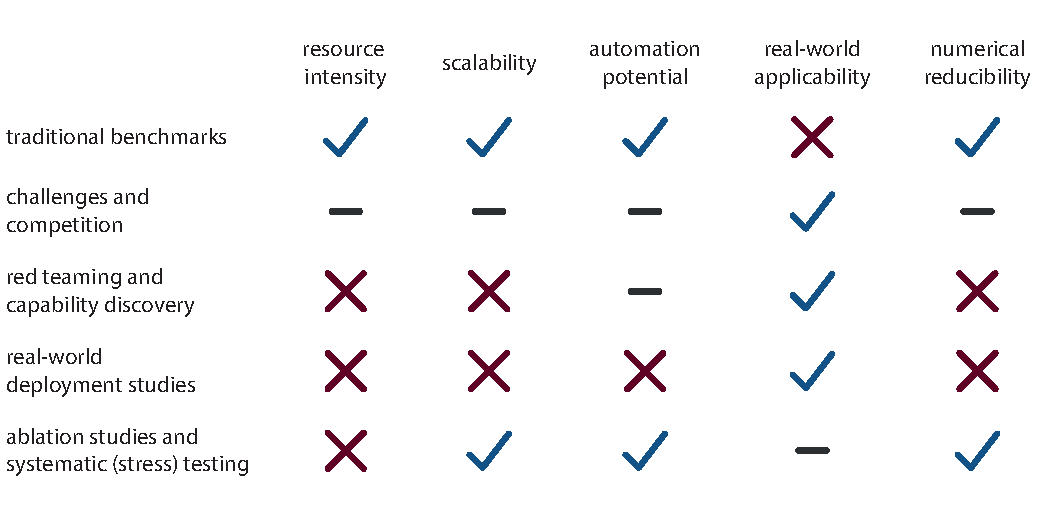
\includegraphics[width=1\textwidth]{figures/rescaled_figures/chemrev_figure10.pdf}
    \caption{\textbf{Comparison of Evaluation Methodologies}: This figure compares five common evaluation methodologies for \glspl{gpm} across the dimensions of resource intensity (required human and computational effort), scalability (ease of applying the method across tasks and models), automation potential (need for manual intervention), real-world applicability (alignment with practical use cases), and numerical reducibility (ability to express results quantitatively). Checkmarks indicate a strength in the respective dimension, crosses denote a limitation, and dashes represent a neutral position.}

\end{figure}

\paragraph{Traditional Benchmarks}\label{para:trad_benchmarks}
Traditional benchmarks can provide a fast and scalable evaluation of the models. In the context of \gls{ml}, a benchmark typically refers to a curated collection of tasks or questions alongside a defined evaluation protocol, which allows different models to be compared under the same conditions. 
Despite their advantages, summarized in \Cref{fig:estimators}, benchmarks come with several limitations. They often struggle to capture real-world impact, as they evaluate models in controlled environments that may not reflect the complexity and open-endedness of real-world applications. Current chemistry benchmarks like ChemBench\autocite{mirza2024large} and CAMEL - Chemistry\autocite{li2023camel} mostly fall on the pragmatic side of the measurement spectrum, as they are designed for comparison and decision-making rather than assessing inherent model properties. 
Classical benchmarks such as \modelname{MoleculeNet} \autocite{wu2018moleculenet} typically target molecular properties---such as solubility or binding affinity---that are experimentally measurable and representationally grounded. However, their evaluation setup, which relies on static and narrowly defined datasets, often fails to capture real-world applicability.

An additional disadvantage of traditional benchmarks is ease of overfitting, where models are optimized for high scores rather than genuine improvements. 
This problem is closely linked to data leakage---also known as test set pollution---which refers to the unintentional incorporation of test set information into the training process. Such leakage can distort performance estimates, especially when models are trained on publicly available benchmarks.\autocite{thompson2025chatbots}
This exposure increases the risk that models learn to perform well on specific benchmark questions rather than developing a deeper, more generalizable understanding of the underlying concepts, leading to an overestimation of their true capabilities. 

Several strategies have been proposed to mitigate these issues. One approach is to keep a portion of the benchmark private, preventing models from being exposed to evaluation data during training---as implemented in \modelname{LAB-Bench}, where $20\%$ of the questions are held out to safeguard against data leakage and overfitting.\autocite{laurent2024lab0bench0} 
Alternatively, some initiatives explore privacy-preserving methods or the use of trusted third parties to evaluate models on held-out data without releasing it publicly. \autocite{eleutherai2024thirdparty}
Another strategy is to regularly update benchmarks by introducing more difficult or diverse tasks over time. \autocite{jimenez2023swe} 
While this helps reduce overfitting by continually challenging models, it complicates long-term comparisons across versions and can undermine stability in performance tracking. \autocite{alampara2025lessons}

Another limitation is that most benchmarks force models to respond to every question, even when uncertain, preventing evaluation of their ability to recognize what they do not know---an essential skill in real-world settings. \modelname{LAB-Bench} addresses this by allowing models to abstain via an \enquote{insufficient information} option, enabling a more nuanced assessment that distinguishes between confident knowledge and uncertainty.


\paragraph{Challenges and Competitions}
Competitions and challenges offer a structured way to evaluate models under realistic conditions, emphasizing prospective prediction and reducing overfitting risks.\autocite{Moult2005} 
Participants typically must submit predictions for a hidden test set, enabling blind, fair evaluation that more closely mirrors real-world deployment. Unlike standard benchmarking setups, these challenges often involve tasks with temporal, external, or domain-specific novelty, making them more resistant to subtle data leakage or overfitting through test set familiarity. 
While such challenges allow for systematic and rigorous assessment of model capabilities, they also require substantial coordination and oversight by a trusted third party.

Such challenges have been rare in chemistry to date, though recent examples in areas like polymer property prediction \autocite{gang2025neurips} suggest this is beginning to change. 
More successful examples exist in related domains---most notably the \gls{caspr} competition\autocite{Moult2005} for protein structure prediction in biology, and the crystal structure prediction blind test challenge\autocite{Lommerse2000} in materials science.

\paragraph{Red Teaming and Capability Discovery} \label{para:red_teaming}
Red teaming focuses on testing models in ways that they were not explicitly designed for, often probing their weaknesses, as well as unintended and unknown behaviors. \autocite{perez2022red, ganguli2022red} 
This group of evaluations includes attempts to bypass alignment mechanisms through adversarial prompting---deliberate attempts to elicit harmful, unsafe, or hidden model outputs by manipulating the input in subtle ways---or to reveal unintended capabilities. \autocite{zhu2023prompt, kumar2023computation} 
Unlike standardized benchmarks, red teaming can reveal model abilities that remain undetected in evaluations with predefined tasks. However, a major challenge is the lack of systematic comparability. 
Results often depend on specific test strategies and are harder to quantify across models. Currently, most red teaming is conducted by human experts, making it a time-consuming process. Automated approaches are emerging to scale these evaluations, \autocite{ge2023mart0}, but in domains like chemistry, effective automation requires models to possess deep scientific knowledge, which remains a significant challenge. 

A concrete example of red teaming in chemistry was presented in the \modelname{GPT-4} Technical Report \autocite{openai2023gpt04}. 
By augmenting \modelname{GPT-4} with tools like molecule search, synthesis planning, literature retrieval, and purchasability checks, red-teamers were able to identify purchasable chemical analogs of a given compound, and even managed to have one delivered to a home address. 
While the demonstration used a benign leukemia drug, the same approach could, in principle, be applied to identify alternatives to harmful substances.\autocite{urbina2022dual}

\paragraph{Real-World Deployment Studies} 
Real-world deployment studies evaluate models in practical use settings, such as testing a \gls{gpm} in a laboratory environment. \autocite{he2020deployment}
Unlike controlled benchmarks, these studies provide insights into how models perform in dynamic, real-world conditions, capturing challenges that predefined evaluations may overlook. 
For example, a generative model might be used to suggest synthesis routes that are then tested experimentally, revealing failures due to overlooked side reactions or missing reaction feasibility. However, they come with significant drawbacks: they are highly time-consuming, and systematic comparisons between models are difficult, as real-world environments introduce variability that is hard to control. 

To date, such evaluations remain rare in the chemical sciences. 


\paragraph{Ablation Studies and Systematic Testing} 
Ablation studies analyze models by systematically isolating and testing individual components or capabilities. 
By removing or modifying specific parts of the models, the impact on performance can be evaluated, providing information on the model’s functionality and potential weaknesses. This approach can be relatively scalable and structured, allowing for thorough and reproducible assessments. Ablation studies reveal limitations and improve overall reliability by ensuring a deeper understanding of how different elements contribute to the model’s behavior. 

\textcite{alampara2024probing} conducted ablation studies to isolate the effects of scientific terminology, task complexity, and prompt guidance on model performance in multimodal chemistry tasks. 
In \modelname{MaCBench}, they showed that removing scientific terms or adding explicit guidance substantially improved model accuracy, suggesting that current models often rely on shallow heuristics rather than deep understanding. These structured ablations highlight specific failure modes and inform targeted improvements in prompt design and training strategies.

\subsection{Future Directions}

\paragraph{Emerging Evaluations Needs} To evaluate \glspl{gpm} in real-world conditions, more open-ended, multimodal, and robust approaches are needed. This is particularly evident in chemistry, where meaningful tasks often extend beyond text and require interpreting molecular structures, reaction schemes, or lab settings.
Here, vision plays a fundamental role, enabling perception and reasoning in complex environments---such as reading labels, observing color changes, or manipulating an apparatus. \autocite{Eppel2020computer}
In addition to visual cues, auditory signals---such as timer alerts or mechanical noise---can play a critical role in ensuring safety and coordination in lab environments. 
Sensorimotor input may also be relevant for simulating or guiding physical manipulation tasks, such as pipetting, adjusting equipment, or following multistep experimental procedures.


Beyond multimodality, another crucial challenge lies in evaluating open-ended scientific capabilities. 
Unlike well-defined benchmarks with fixed answers, real-world scientific inquiry is inherently open-ended.\autocite{mitchener2025bixbench0} This not only demands flexible and adaptive evaluation schemes but also raises deeper questions about what constitutes scientific understanding in generative models. 
This becomes even more important as agent-based systems (\Cref{sec:agents} gain traction---models that do not simply respond to prompts but autonomously plan, reason, and execute multistep tasks in interaction with tools, databases, and lab environments. \autocite{cao2024agents, mandal2024autonomous}
Simple input-output benchmarks are insufficient; instead, we need frameworks that can track progress in dynamic, goal-driven settings, where multiple valid solutions may exist. 

In parallel to capability assessments, the evaluation of safety (see \Cref{sec:safety}) is becoming increasingly important---especially as \glspl{gpm} gain access to sensitive scientific knowledge and tools.\autocite{bran2024augmenting, boiko2023autonomous} 
Current safety evaluations often rely on manual red teaming \Cref{sec:eval_methods}, which is neither scalable nor systematic. 
Future evaluation frameworks must therefore include robust, automated, and scalable safety testing pipelines, capable of detecting misuse potential and risky behaviors across modalities and contexts.\autocite{goldstein2023generative}

Moreover, evaluations should not be limited to static benchmarks.
One promising avenue could be the organization of recurring community-wide challenges, similar to established competitions in other fields (e.g., \gls{caspr}\autocite{Moult2005}). These challenges---ideally coordinated by major research consortia or national labs---can serve as shared reference points, drive innovation in evaluation design.

\paragraph{Standardization Efforts} One persistent challenge in evaluating \glspl{gpm} is the lack of common standards---whether in benchmark design, metric selection, or reporting protocols. This fragmentation makes it challenging to compare results or ensure reproducibility. 
While some degree of standardization can support transparency and cumulative progress, rigid frameworks risk constraining innovation and may conflict with the need in scientific discovery for more open-ended, adaptive evaluations. 

A more feasible path may lie in promoting transparent documentation of evaluation choices and developing meta-evaluation tools that assess the validity, coverage, and robustness of different approaches. Emerging frameworks such as \gls{irt} offer promising directions for such reflective evaluations, enabling nuanced insights beyond surface-level metrics. \autocite{schilling2025lifting}


\section{Applications}

\subsection{Automating the Scientific Workflow} \label{sec:ai-scientists}

Recent advances in \glspl{gpm}, particularly \glspl{llm}, have enabled initial demonstrations of fully autonomous \gls{ai} scientists \autocite{schmidgall2025agent}. 
We define these as \gls{llm}-powered architectures capable of executing end-to-end research workflows based solely on the final objectives, e.g., \enquote{\textit{Unexplained rise of antimicrobial resistance in Pseudomonas. Formulate hypotheses, design confirmatory in vitro assays, and suggest repurposing candidates for liver-fibrosis drugs}}. 
Such systems navigate partially or entirely through all components of the scientific process outlined in \Cref{fig:applications}, and detailed in the subsequent sections. 

While significant applications emerge in \gls{ml} and programming, scientific implementations remain less explored.

\subsubsection{Coding and ML Applications of AI Scientists}

Notable frameworks, including \modelname{Co-Scientist} \autocite{gottweis2025towards}, and \modelname{\gls{ai}-Scientist} \autocite{yamada2025ai}, aim to automate the entire \gls{ml} research pipeline, typically employing multi-agent architectures (described in detail in \Cref{sec:multi-agent}) where specialized agents manage distinct phases of the scientific method \autocite{schmidgall2025agentrxiv}. 
Critical to these systems is self-reflection \autocite{renze2024self0reflection}---iterative evaluation and criticism of results within validation loops. 
However, comparative analyses reveal that \gls{llm}-based evaluations frequently overscore outputs relative to human assessments \autocite{huang2023mlagentbench0, chan2024mle, starace2025paperbench0}. 
From an engineering perspective, alternative approaches focus specifically on iterative code optimization, enabling systems to refine their codebases \autocite{zhang2025darwin} or generate improved agents autonomously \autocite{hu2024automated}.
In another work, \modelname{AlphaEvolve} \autocite{novikov2025alphaevolve}, which is an \gls{llm} operating within a \gls{ga} environment, found novel algorithms for matrix multiplication (which had seen no innovation in fifty years) and sorting.

\subsubsection{Chemistry and Related Fields}

In chemistry, proposed systems show promising results. \modelname{Robin} identified ripasudil as a treatment for \gls{damd} \autocite{ghareeb2025robin0}---despite pending clinical trials and the general debate for these systems about novelty of their findings\autocite{Listgarten2024perpetual}.
However, automation of experiment execution poses a major constraint for the chemistry-focused \gls{ai}-scientists due to hardware requirements, making computational chemistry the most feasible subfield in which agents have successfully run simple quantum simulations \autocite{Zou2025ElAgente}. 
Further, the \glspl{llm} powering these systems exhibit limited chemical knowledge \autocite{mirza2024large}. 
Despite this, \modelname{ether0} \autocite{narayanan2025training}---the first chemistry-specialized reasoning \gls{llm} (see \Cref{sec:rl} for a deeper discussion on reasoning models)---demonstrated strong capabilities in molecular design and accurate reaction prediction, positioning it as a promising foundation for chemistry-focused \gls{ai} scientists.

\subsubsection{Are these Systems Capable of Real Autonomous Research?}

Although agents like \modelname{Zochi} \autocite{intologyai2025zochi} achieved peer-reviewed publication in top-tier venues (\gls{acl} 2025), their capacity for truly autonomous end-to-end research remains debatable \autocite{son2025ai}. 
Even when generating hypotheses that appear novel and impactful, their execution and reporting of these ideas, as demonstrated by \textcite{si2025ideation1execution}, yield results deemed less attractive than those produced by humans. Additionally, this autonomy raises a critical question: \textit{What should the role of \gls{ai} in science be?} 
While these systems can generate hypotheses, conduct experiments, and produce publication-ready manuscripts, their integration demands careful consideration (refer to \Cref{sec:ethics} for further discussion about moral concerns around these systems). 
Beyond the vision of fully autonomous scientists, \glspl{gpm}---primarily \glspl{llm}---are already utilized across most scientific workflow components, for which \glspl{llm} have proven useful for some. 
These elements are shown in \Cref{fig:applications}, and we discuss next.


\begin{figure}[!ht]
    \centering
    \label{fig:applications}
    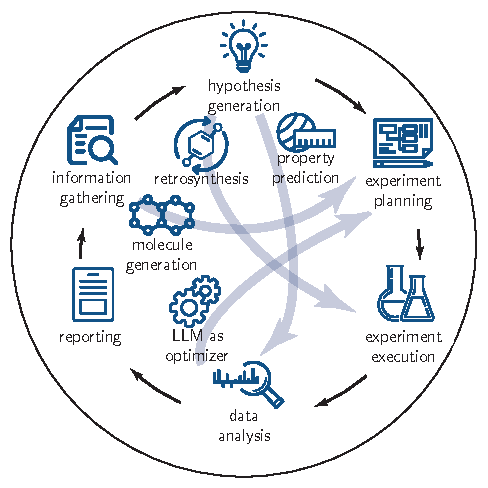
\includegraphics[width=0.5\textwidth]{figures/rescaled_figures/chemrev_figure11.pdf}
    \caption{\textbf{Overview of the scientific process}. The outer elements represent the typical scientific research process: from gathering information and generating hypotheses based on the observations, to executing experiments and analyzing the results. The terms that are in the center represent data-driven \enquote{shortcuts} that \enquote{accelerate} the typical scientific method. All stages represented in the figure are discussed in detail in the following sections.}
\end{figure}

\subsection{Existing GPMs for Chemical Science}

The development of \glspl{gpm} for chemical science represents a departure from traditional single-task approaches. Rather than fine-tuning pre-trained models for specific applications such as property prediction or molecular generation, these chemistry-aware language models are intentionally designed to perform multiple chemical tasks simultaneously. This multitask paradigm offers several advantages: shared representations across related chemical problems\autocite{dimitrios2023unifying}, improved data efficiency through transfer learning between tasks\autocite{lim2021predicting}, and the potential for emergent capabilities that arise from joint training across diverse chemical domains\autocite{livne2024nach0}.

\paragraph{Multitask Learning Frameworks} \modelname{DARWIN 1.5} pioneered the multitask approach by fine-tuning \modelname{Llama-7B} through a two-stage process \autocite{xie2025darwin}. Initially trained on 332k scientific question-answer pairs to establish foundational scientific reasoning, the model subsequently underwent multitask learning to perform property prediction-related regression and classification tasks concurrently.

Building on similar principles, \modelname{nach0} introduced a unified encoder-decoder transformer architecture for cross-domain chemical tasks \autocite{livne2024nach0}. Pre-trained using \gls{ssl} on both natural language and chemical data, \modelname{nach0} tackles diverse downstream applications including molecular structure generation, chemical property prediction, and reaction prediction. Notably, the authors found that combining chemistry-specific tasks outperformed models trained on distinct task groups, suggesting that chemical reasoning benefits from focused domain integration.

In the materials domain, \textcite{qu2023leveraging} developed a language-driven materials discovery framework that uses transformer-based embeddings (e.g., \modelname{MatBERT}\autocite{wan2024tokens}) to represent and generate novel crystal structures. Candidates are first recalled via similarity in embedding space, then ranked using a multitask multi-gate \gls{moe} model that predicts the desired properties jointly. 
Their method successfully identifies novel high-performance materials (e.g., halide perovskites) and demonstrates that language representations encode latent knowledge for task-agnostic materials design.

\paragraph{Domain-Specific Pre-Training Strategies} A second category of \glspl{gpm} emphasizes deep domain knowledge through specialized pre-training. \modelname{LLaMat} employed \gls{peft} specifically on crystal structure data in \gls{cif} format, enabling the generation of thermodynamically stable structures \autocite{mishra2024foundational}.

\modelname{ChemDFM} scales this concept significantly, implementing domain pre-training on over 34 billion tokens from chemical textbooks and research articles \autocite{zhao2024chemdfm}. Through comprehensive instruction tuning, \modelname{ChemDFM} familiarizes itself with chemical notation and patterns, distinguishing it from more materials-focused approaches like \modelname{LLaMat} through its broader chemical knowledge base.

\modelname{ChemLLM} further refined this approach by introducing template-based instruction tuning (ChemData) to optimize property-guided molecular generation \autocite{zhang2024chemllm}.

\paragraph{Reasoning-Based Approaches} A recent development in chemical \glspl{gpm} incorporates explicit reasoning capabilities. \modelname{ether0} demonstrates this approach as a 24 billion parameter reasoning model trained on over 640k experimentally-grounded chemistry problems across diverse tasks, including retrosynthesis, solubility editing, and property prediction \autocite{narayanan2025training}. 
Unlike previous models, \modelname{ether0} uses \gls{rl} (see \Cref{sec:rl}) to develop reasoning behaviors like verification and backtracking, demonstrating that structured problem-solving approaches can significantly improve performance on complex chemical tasks while maintaining grounding in experimental data.

These diverse approaches illustrate the evolving landscape of chemical \glspl{gpm}, each balancing broad applicability with domain-specific precision.
Still, most applications of \glspl{gpm} focus on using these models for one specific application and we will review those in the following.

\subsection{Knowledge Gathering}\label{sec:information_gathering}
The rate of publishing keeps growing, and as a result, it is increasingly challenging to manually collect all relevant knowledge, potentially stymying scientific progress.\autocite{schilling2025text, Chu_2021}
Even though knowledge collection might seem like a simple task, it often involves multiple different steps, visually described in \Cref{fig:knowledge_gathering}. We split the discussion in this section in two: structured data extraction and question answering. Example queries for both sections are in \Cref{fig:knowledge_gathering}B.

\begin{figure}[!ht]
    \centering
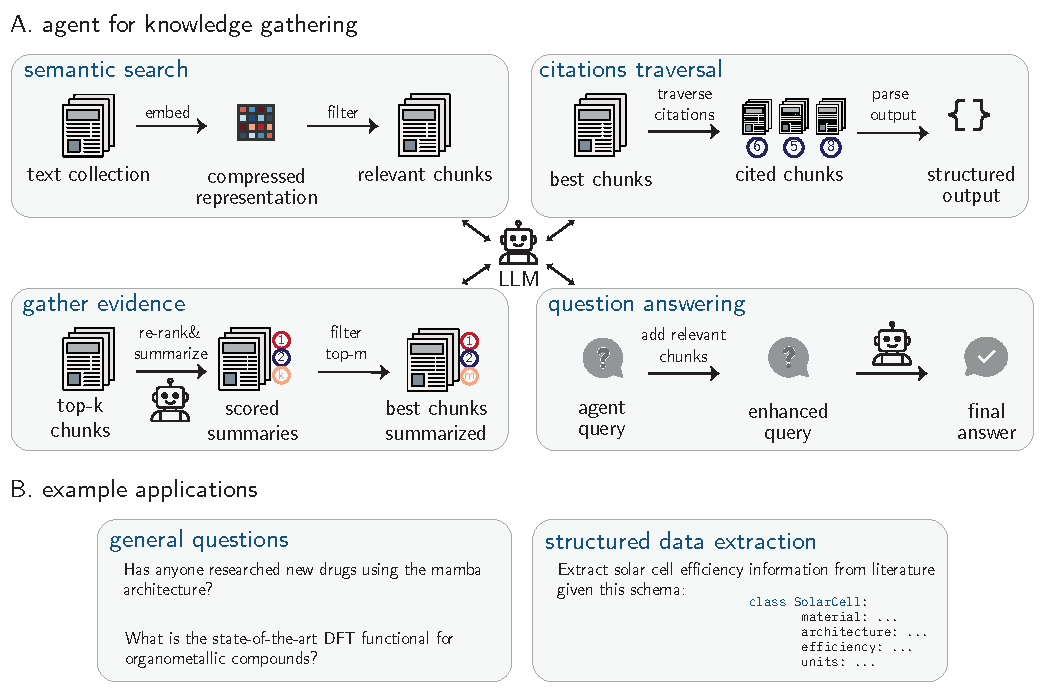
\includegraphics[width=1\textwidth]{figures/rescaled_figures/chemrev_figure12.pdf}
    \caption{\textbf{A. a representation of a typical agent for scientific queries.} The \gls{llm} is the central piece of the system, surrounded by typical tools that improve its question-answering capabilities, together forming an agentic system. The tools represented in this figure are semantic search, citation traversal, evidence gathering, and question answering. Semantic search finds relevant documents. Evidence gathering ranks and filters chunks of text using \glspl{llm}. The citation traversal tool provides model access to citation graphs, enabling accurate referencing of each chunk and facilitating the discovery of additional sources. Finally, the question-answering tool (an \gls{llm}) collects all the information found by other tools and generates a final response to a user's query. This part the figure is inspired by the \modelname{PaperQA2} agent.\autocite{skarlinski2024language} \textbf{B.} two examples of applications discussed in this section.}
\label{fig:knowledge_gathering}
\end{figure}


\paragraph{Semantic Search} A step that is key to most, if not all, knowledge-gathering tasks is \gls{rag}, discussed in more detail in \Cref{sec:rag}. 
Most commonly, this involves semantic search, intended to identify chunks of text with similar meaning. 
The difference between semantic search and conventional search lies in how each approach interprets queries. The latter operates through lexical matching---whether exact or fuzzy---focusing on the literal words and their variations. Semantic search, however, goes deeper by interpreting the underlying meaning and contextual relationships within the content. 

To enable semantic search, documents are stored in vector databases using embedding vectors (see \Cref{sec:embeddings}).\autocite{bojanowski2017enriching} 
They represent the content of a document as a vector in a learned vector space and hence allow for similarity search by vector comparison (e.g., using cosine similarity for small databases or more sophisticated algorithms like \gls{hnsw} for large databases\autocite{malkov2018efficient}). 

In chemistry, semantic search has been used extensively to classify and identify chemical text.\autocite{Guo2021,beltagy2019scibert0,trewartha2022quantifying}

\subsubsection{Structured Data Extraction}

Semantic search can help us find relevant resources. 
However, for many applications it can be useful to collect data in a structured form, e.g., tables with fixed columns.
Obtaining such a dataset based on extracting data from the literature using \glspl{llm} is currently one of the most practical avenues for the use of \glspl{llm} in the chemical sciences \autocite{schilling2025text}.
Currently, \glspl{llm} are used in various forms for this application. 

\paragraph{Data Extraction Using Prompting} 

For most applications, zero-shot prompting should be the starting point. In this context, zero-shot prompting has been used to extract data about organic reactions\autocite{rios2025llm,vangala2024suitability, Patiny2023automatic}, synthesis procedures for metal-organic frameworks\autocite{zheng2023chatgpt}, polymers\autocite{schilling2024using,gupta2024data}, solar cells\autocite{shabih2025automated}, or materials data\autocite{polak2024extracting,hira2024reconstructing,kumar2025mechbert,wu2025large,huang2022batterybert}. 
 
\paragraph{Fine-tuning Based Data Extraction} 

If a commercial model needs to be run very often, it can be more cost-efficient to fine-tune a smaller, open-source model compared to prompting a large model. 
In addition, models might lack specialized knowledge and might not follow certain style guides, which can be introduced with fine-tuning. 
\textcite{ai2024extracting} fine-tuned the \modelname{LLaMa-2-7B} model to extract procedural chemical reaction data from \gls{uspto}, and converted it to a \gls{json} format compatible with the schema of \gls{ord}\autocite{Kearnes_2021}, achieving an overall accuracy of more than $90\%$. 
In a different work, \textcite{zhang2024fine} fine-tuned \modelname{GPT-3.5-Turbo} to recognize and extract chemical entities from \gls{uspto}. Fine-tuning improved the performance of the base model on the same task by more than $15\%$. Similarly, \textcite{dagdelen2024structured} proposed a human-in-the-loop data annotation process, where humans correct the outputs from an \gls{llm} extraction instead of extracting data from scratch.

\paragraph{Agents for Data Extraction} 

Agents (\Cref{sec:agents}) have shown their potential in data extraction, though to a limited extent.\autocite{chen2024autonomous,kang2024chatmof}
For example, \textcite{ansari2024agent} introduced \modelname{Eunomia}, an agent that autonomously extracts structured materials science data from scientific literature without requiring fine-tuning, demonstrating performance comparable to or better than fine-tuned methods. Their agent is an \gls{llm} with access to tools such as chemical databases (e.g., the \modelname{Materials Project} database) and research papers from various sources.

While the authors claim this approach simplifies dataset creation for materials discovery, the evaluation is limited to a narrow set of materials science tasks (mostly focusing on \glspl{mof}), indicating the need for the creation of agent evaluation tools.


\paragraph{Limitations} 
The ability to extract data from sources other than text is important since a large amount of data is only stored in plots, tables, and figures. 
Despite some initial simple proofs of concept \autocite{Zheng2024image}, the main bottleneck presently is the limited understanding of image data compared to text data in multimodal models.\autocite{alampara2024probing} The promise of agents lies in their ability to interact with tools (that can also interpret multimodal data). Moreover, their ability to self-reflect could automatically improve wrong results.\autocite{du2023improving}

\subsubsection{Question Answering}
Besides extracting information from documents in a structured format, \glspl{llm} can also be used to answer questions---such as \enquote{Has X been tried before} by synthesizing knowledge from a corpus of documents (and potentially automatically retrieving additional documents). 

An example of a system that can do that is \modelname{PaperQA}. This agentic system contains tools for search, evidence-gathering, and question answering as well as for traversing citation graphs, which are shown in \Cref{fig:knowledge_gathering}. The evidence-gathering tool collects the most relevant chunks of information via the semantic search and performs \gls{llm}-based re-ranking of these chunks (i.e. the \gls{llm} changes the order of the chunks depending on what is needed to answer the query).
Subsequently, only the top-$n$ most relevant chunks are kept. To further ground the responses, citation traversal tools (e.g., Semantic Scholar\autocite{kinney2023semantic}) are used. 
These leverage the citation graph as a means of discovering supplementary literature references. Ultimately, to address the user's query, a question-answering tool is employed. It initially augments the query with all the collected information before providing a definitive answer.
The knowledge aggregated by these systems could be used to generate new hypotheses or challenge existing ones. 
Thus, in the next section, we focus on this aspect.


\subsection{Hypothesis Generation} \label{sec:hypothesis-gen}

Coming up with new hypotheses represents a cornerstone of the scientific process \autocite{rock2018hypothesis}. Historically, hypotheses have emerged from systematic observation of natural phenomena, exemplified by Isaac Newton’s formulation of the law of universal gravitation \autocite{newton1999principia}, which was inspired by the seemingly mundane observation of a falling apple \autocite{kosso2017whatgoesup}.

In modern research, hypothesis generation increasingly relies on data-driven tools. 
For example, clinical research employs frameworks such as \gls{viads} to derive testable hypotheses from well-curated datasets \autocite{Jing2022roles}. Similarly, advances in \glspl{llm} are now being explored for their potential to automate and enhance idea generation across scientific domains \autocite{oneill2025sparks}. However, such approaches face significant challenges due to the inherently open-ended nature of scientific discovery \autocite{stanley2017openendedness}. 
Open-ended domains, as discussed in \Cref{sec:data-section}, risk intractability, as an unbounded combinatorial space of potential variables, interactions, and experimental parameters complicates systematic exploration \autocite{clune2019ai0gas0}.
Moreover, the quantitative evaluation of the novelty and impact of generated hypotheses remains non-trivial. 
As Karl Popper argued, scientific discovery defies rigid logical frameworks \autocite{popper1959logic}, and objective metrics for \enquote{greatness} of ideas are elusive \autocite{stanley2015greatness}. These challenges underscore the complexity of automating or systematizing the creative core of scientific inquiry.

\subsubsection{Initial Sparks}

Recent efforts in the \gls{ml} community have sought to simulate the hypothesis formulation process \autocite{Gu2025forecasting, arlt2024meta0designing}, primarily leveraging multi-agent systems \autocite{jansen2025codescientist0, kumbhar2025hypothesis}. 
In such frameworks, agents typically retrieve prior knowledge to contextualize previous related work---grounding hypothesis generation in existing literature \autocite{naumov2025dora, ghareeb2025robin0, gu2024interesting}. 
A key challenge, however, lies in evaluating the generated hypotheses. 
While some studies leverage \glspl{llm} to evaluate novelty or interestingness \autocite{zhang2024omni0}, recent work has introduced critic agents---specialized components designed to monitor and iteratively correct outputs from other agents---into multi-agent frameworks (see \Cref{sec:multi-agent}). 
For instance, \textcite{Ghafarollahi2024} demonstrated how integrating such critics enables systematic hypothesis refinement through continuous feedback mechanisms.

However, the reliability of purely model-based evaluation remains contentious. 
\textcite{si2025llms} argued that relying on a \gls{gpm} to evaluate hypotheses lacks robustness, advocating instead for human assessment. 
This approach was adopted in their work, where human evaluators validated hypotheses produced by their system, finding more novel \gls{llm}-produced hypotheses compared to the ones proposed by humans.
Notably, \textcite{yamada2025ai} advanced the scope of such systems by automating the entire research \gls{ml} process, from hypothesis generation to article writing. 
Their system’s outputs were submitted to workshops at the \gls{iclr} 2025, with one contribution ultimately accepted. However, the advancements made by such works are currently incremental instead of unveiling new, paradigm-shifting  research (see \Cref{fig:hypothesis-generation}).

\subsubsection{Chemistry-Focused Hypotheses}

In scientific fields such as chemistry and materials science, hypothesis generation requires domain intuition, mastery of specialized terminology, and the ability to reason through foundational concepts \autocite{miret2024llms}. 
To address potential knowledge gaps in \glspl{llm}, \textcite{wang2023scimon0} proposed a few-shot learning approach (see \Cref{sec:prompting}) for hypothesis generation and compared it with model fine-tuning for the same task. 
Their method strategically incorporates in-context examples to supplement domain knowledge while discouraging over-reliance on existing literature. 
For fine-tuning, they designed a loss function that penalizes possible biases---e.g., given the context \enquote{hierarchical tables challenge numerical reasoning}, the model would be penalized if it generated an overly generic prediction like \enquote{table analysis} instead of a task-specific one---when trained on such examples. 
Human evaluations of ablation studies revealed that \modelname{GPT-4}, augmented with a knowledge graph of prior research, outperformed fine-tuned models in generating hypotheses with greater technical specificity and iterative refinement of such hypotheses.

Complementing this work, \textcite{yang2025moose} introduced the \modelname{Moose-Chem} framework to evaluate the novelty of \gls{llm}-generated hypotheses. 
To avoid data contamination, their benchmark exclusively uses papers published after the knowledge cutoff date of the evaluated model, \modelname{GPT-4o}. 
Ground-truth hypotheses were derived from articles in high-impact journals (e.g., Nature, Science) and validated by domain-specialized PhD researchers.
By iteratively providing the model with context from prior studies, \modelname{GPT-4o} achieved coverage of over $80\%$ of the evaluation set’s hypotheses while accessing only $4\%$ of the retrieval corpus, demonstrating efficient synthesis of ideas presumably not present in its training corpus.

\begin{figure}[!ht]
    \centering
        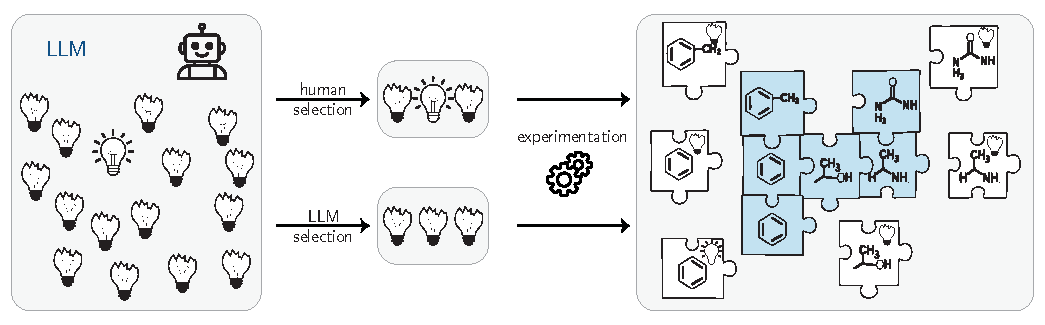
\includegraphics[width=1\textwidth]{figures/rescaled_figures/chemrev_figure13.pdf}
    \caption{\textbf{Overview of \gls{llm}-based hypothesis generation}. 
    Current methods are based on \gls{llm}-sampling methods in which an \gls{llm} proposes new hypotheses. 
    The generated hypotheses are evaluated in terms of novelty and impact either by another \gls{llm} or by a human. Then, through experimentation, the hypotheses are transformed into results which showcase that current \glspl{llm} cannot produce groundbreaking ideas, limited to their training corpus, resulting in the best cases, in incremental work. This is shown metaphorically with the puzzle. The \enquote{pieces of chemical knowledge} based on the hypothesis produced by \glspl{llm} are already present in the \enquote{chemistry puzzle}, not unveiling new parts of it.}
    \label{fig:hypothesis-generation}
\end{figure}

\subsubsection{Are LLMs Actually Capable of Novel Hypothesis Generation?}

Automatic hypothesis generation is often regarded as the Holy Grail of automating the scientific process \autocite{coley2020autonomous}. However, achieving this milestone remains challenging, as generating novel and impactful ideas requires questioning current scientific paradigms \autocite{Kuhn1962Structure}---a skill typically refined through years of experience---which is currently impossible for most \gls{ml} systems.

Current progress in \gls{ml} illustrates these limitations \autocite{kon2025exp0bench0, gu2024interesting}. Although some studies claim success in \gls{ai}-generated ideas accepted at workshops in \gls{ml} conferences via double-blind review \autocite{zhou2025tempest0}, these achievements are limited. 
First, accepted submissions often focus on coding tasks, one of the strongest domains for \glspl{llm}. Second, workshop acceptances are less competitive than main conferences, as they prioritize early-stage ideas over rigorously validated contributions. 
In chemistry, despite some works showing promise on these systems \autocite{yang2025moose0chem20}, \glspl{llm} struggle to propose functional hypotheses \autocite{si2025ideation1execution}.
Their apparent success often hinges on extensive sampling and iterative refinement, rather than genuine conceptual innovation.

As \textcite{Kuhn1962Structure} argued, generating groundbreaking ideas demands challenging prevailing paradigms---a capability missing in current \gls{ml} models (they are trained to make the existing paradigm more likely in training rather than questioning their training data), as shown in \Cref{fig:hypothesis-generation}. 
Thus, while accidental discoveries can arise from non-programmed events (e.g., Fleming’s identification of penicillin \autocite{Fleming1929antibacterial, Fleming1945penicillin}), transformative scientific advances typically originate from deliberate critique of existing knowledge \autocite{popper1959logic, Lakatos1970falsification}. In addition, very often breakthroughs can also not be achieved by optimizing for a simple metric---as we often do not fully understand the problem and, hence, cannot design a metric.\autocite{stanley2015greatness}
Despite some publications suggesting that \gls{ai} scientists already exist, such claims are supported only by narrow evaluations that yield incremental progress \autocite{novikov2025alphaevolve}, not paradigm-shifting insights. For \gls{ai} to evolve from research assistants into autonomous scientists, it must demonstrate efficacy in addressing societally consequential challenges, such as solving complex, open-ended problems at scale (e.g., \enquote{millennium} math problems
\autocite{Carlson2006millennium}).

Finally, ethical considerations become critical as hypothesis generation grows more data-driven and automated. Adherence to legal and ethical standards must guide these efforts (see \Cref{sec:safety}) \autocite{danish_gov2024hypothesis}.

With a hypothesis in hand, the next step is often to run an experiment to test it. 


\subsection{Experiment Planning}
\label{sec:planning}
Before a human or robot can execute any experiments, a plan must be created. 
Planning can be formalized as the process of decomposing a high-level task into a structured sequence of actionable steps aimed at achieving a specific goal. 
The term planning is often confused with scheduling and \gls{rl}, which are closely related but distinct concepts. Scheduling is a more specific process focused on the timing and sequence of tasks. 
It ensures that resources are efficiently allocated, experiments are conducted in an optimal order, and constraints (such as lab availability, time, and equipment) are respected.\autocite{kambhampati2023llmplanning} 
\gls{rl} is about adapting and improving plans over time based on ongoing results.\autocite{chen2022deep}

\subsubsection{Conventional Planning} 
Early experimental planning in chemistry relied on human intuition and domain expertise. 
One example of this is retrosynthesis. 
Since the 1960s, systems like \gls{lhasa} \autocite{corey1972computer} began automating retrosynthesis using hand-coded rules and heuristics\autocite{warr2014short}. 
Later tools, such as \modelname{Chematica}\autocite{grzybowski2018chematica}, expanded these efforts by integrating larger template libraries and optimization strategies. 
As reaction data grew in volume and complexity, manual rule encoding became unsustainable. 
Platforms like ASKCOS\autocite{tu2025askcos} integrated \glspl{gnn} and neural classifiers to predict reactivity and suggest conditions, enabling actionable synthetic routes. 

All applications, however, face the problem that planning is difficult because search spaces are combinatorially large and evaluating potential paths, in principle, requires a model that can perfectly predict the outcomes of different actions. Conventional approaches often rely on various forms of search algorithms such as \gls{bfs}, \gls{dfs}, \gls{mcts} \autocite{segler2017towards}. 
Those, however, are often still not efficient enough to tackle long-horizon planning for complex problems. 

\subsubsection{LLMs to Decompose Problems into Plans}
\glspl{gpm}, in particular \glspl{llm}, can potentially assist in planning with two modes of thinking. 
Deliberate (system-2-like) thinking can be used to score potential options or to decompose problems into plans. 
Intuitive (system-1-like) thinking can be used to efficiently prune search spaces. 
These two modes align with psychological frameworks known as system-1 and system-2 thinking. \autocite{kahneman2011thinking}
In the system-1 thinking, \glspl{llm} support rapid decision-making by leveraging heuristics and pattern recognition to quickly narrow down options. 
In contrast, system-2 thinking represents a slower, more analytical process, in which \glspl{llm} solve complex tasks---such as logical reasoning and planning---by explicitly generating step-by-step reasoning. \autocite{ji2025test}

Decomposing a goal into actionable milestones relies on this deliberate, system-2-style reasoning, enabling the model to evaluate alternatives and structure plans effectively. 
A variety of strategies have been proposed to improve the reasoning capabilities of \glspl{llm} during inference. 
Methods such as \gls{cot} and least-to-most prompting guide models to decompose problems into interpretable steps, improving transparency and interpretability. 
However, their effectiveness in planning is limited by error accumulation and linear thinking patterns.\autocite{stechly2024chain}
To address these limitations, recent test-time strategies such as repeat sampling and tree search have been proposed to enhance planning capabilities in \glspl{llm}. 
Repeated sampling allows the model to generate multiple candidate reasoning paths, encouraging diversity in thought and increasing the chances of discovering effective subgoal decompositions. \autocite{wang2024planning}
Meanwhile, tree search methods like \gls{tot} and \gls{rap} treat reasoning as a structured search, also using algorithms like \gls{mcts} to explore and evaluate multiple solution paths, facilitating more global and strategic decision-making. \autocite{hao2023reasoning}

Beyond purely linguistic reasoning, \glspl{llm} have also been used to interpret natural-language queries and to translate them into structured planning steps, as demonstrated by systems like \gls{llm}+P\autocite{liu2023llm} and \gls{llm}-DP\autocite{dagan2023dynamic}, which integrated \glspl{llm} with classical planners to convert planning problems into \gls{pddl}.
\glspl{llm} have also been applied to generate structured procedures from limited observations. For example, in quantum physics, a model was trained to infer reusable experimental templates from measurement data, producing Python code that generalized across system sizes. \autocite{arlt2024meta0designing} This demonstrates how \glspl{llm} can support scientific planning by synthesizing high-level protocols from low-level evidence, moving beyond symbolic reasoning to executable plan generation.

\subsubsection{Pruning of Search Spaces}

Pruning refers to the process of eliminating unlikely or suboptimal options during the search to reduce the computational burden.
Because the number of potential pathways can grow exponentially, exhaustive search may be computationally intensive. 
Classical planners employ heuristics, value functions, or logical filters to perform pruning\autocite{bonet2012action}. 
\glspl{llm} can emulate pruning through learned heuristics, intuitive judgment, or context-driven evaluation, \autocite{gao2025synergizing} reflecting system-1 thinking.
\Cref{fig:planning} illustrates how \glspl{llm} can support experimental planning by selectively pruning options.
Rule-based heuristics derived from domain knowledge can automatically discard routes involving unfavorable motifs, such as chemically strained rings or complex aromatic scaffolds. 
Meanwhile, \glspl{llm} can emulate an expert chemist's intuition by discarding synthetic routes that appear unnecessarily long, inefficient, or mechanistically implausible. 

To further enhance planning efficacy, \glspl{llm} can be augmented with external tools that estimate the feasibility or performance of candidate plans, enabling targeted pruning of the search space before costly execution. 
In \modelname{ChemCrow}, the \gls{llm} collaborated with specialized chemical tools with knowledge about molecular and reaction properites. While \modelname{ChemCrow} does not explicitly generate and prune a large pool of candidate plans, these tools serve as real-time evaluators that help the model avoid unfeasible or inefficient directions during synthesis or reaction planning.

In addition to external tools, \glspl{llm} can also engage in self-correction, a reflective strategy that identifies and prunes flawed reasoning steps within their own outputs. 
This introspective pruning supports more robust and coherent planning by discarding faulty intermediate steps before they affect final decisions. 
As such, self-correction offers a lightweight yet effective mechanism for narrowing the solution space in complex reasoning tasks. 
At the highest level of oversight, human-in-the-loop frameworks introduce expert feedback to guide pruning decisions. 
The \modelname{ORGANA} system\autocite{darvish2025organa} integrated chemist feedback into the planning process, helping define goals, resolve ambiguities, and eliminate invalid directions.
\begin{figure}[!htbp]
    \centering
        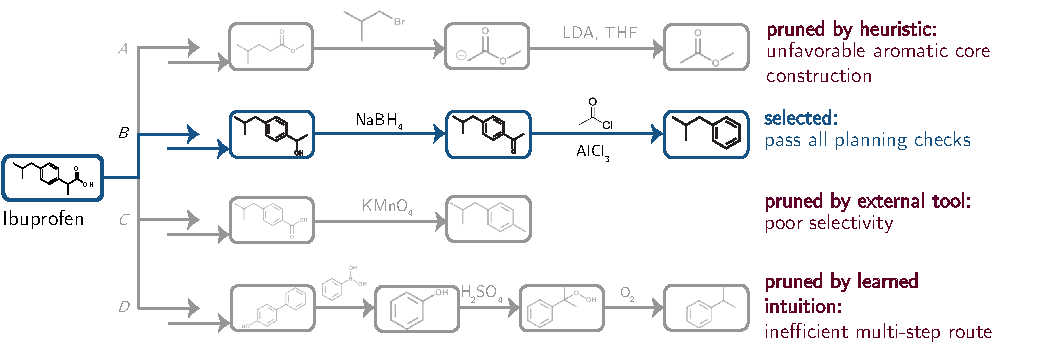
\includegraphics[width=1\textwidth]{figures/rescaled_figures/chemrev_figure14.pdf}
    \caption{\textbf{\gls{gpm}-guided retrosynthesis route planning and pruning}. \glspl{gpm} can systematically evaluate and prune retrosynthetic routes using multiple reasoning capabilities to discriminate between viable and problematic approaches. The partially overlapping arrows at the start of each route indicate multiple steps. \textbf{Route A}: This route was pruned by heuristic reasoning due to the unfavorable aromatic core construction.
    \textbf{Route B}: This route was selected as it successfully passes all \gls{gpm} planning checks, demonstrating optimal synthetic feasibility.
    \textbf{Route C}: This pathway was pruned by external tools due to the poor region-selectivity of the oxidation step.
    \textbf{Route D}: This route was pruned based on learned intuition, as it represents an inefficient multistep pathway; the route could just start with phenol instead of synthesizing it.
}
    \label{fig:planning}
\end{figure}

\subsubsection{Evaluation}
While pruning accelerates planning, its effectiveness depends on reliable evaluation---the ability to judge whether a candidate plan is valid or promising. 
However, evaluating planning quality is particularly challenging in scientific fields such as chemistry and biology. 
Many alternative plans may achieve the same goal, so evaluation is inherently ambiguous in the absence of a comprehensive world model.
In open-ended domains, evaluation is often conducted manually. 
For example, \modelname{ChemCrow} \autocite{bran2024augmenting} relied on expert review to assess the correctness and plausibility of generated outputs. 
More dynamic evaluations can be performed in simulated or real embodied environments \autocite{song2023llm, choi2024lota}, offering interactive feedback on feasibility. 
In parallel, automatic evaluation methods are emerging. 
For example, \modelname{BioPlanner}\autocite{o2023bioplanner}
used pseudocode-based evaluation, comparing \gls{llm}-generated protocols to expert-written pseudocode representations to assess plausibility and correctness without requiring manual review or physical execution.


\subsection{Experiment Execution}
Once an experimental plan is available, whether from a human scientist's idea or a sophisticated AI model, the next step is to execute it. 
Regardless of its source, the plan must be translated into concrete, low-level actions for execution. One of the main challenges of lab automation is to convert the high-level and abstract experimental plan into real-world operations carried out by the experimental hardware (liquid-handing systems, robotic arms, instruments, etc.). 

It is worth noting that, despite their methodological differences, executing experiments \textit{in silico} (running simulations or code) and \textit{in vitro} are not fundamentally different---both follow an essentially identical workflow: Plan $\rightarrow$ Instructions $\rightarrow$ Execution $\rightarrow$ Analysis. 
In a computer simulation, a researcher writes a program (plan), which is then compiled or interpreted into machine code (instructions) for the \gls{cpu}, executed to produce data, and finally the outputs are analyzed. 
In an automated laboratory, the scientist specifies a protocol (plan), which must be translated into instrument commands (instructions), executed on a robotic platform, followed by the analysis of sensor data or assay results. Both scenarios require careful translation of abstract steps into concrete actions, as well as further decision-making based on the acquired results.

The execution of \textit{in silico} experiments can be reduced to two essential steps: preparing input files and running the computational code; \glspl{gpm} can be used in both steps.\autocite{Liu2025ASA, Mendible‑Barreto2025DynaMate, Zou2025ElAgente, Campbell2025MDCrow} \textcite{Jacobs2025orca} found that using a combination of fine-tuning, \gls{cot} and \gls{rag} (see \Cref{sec:model_adaptation}) can improve the performance of \glspl{llm} in generating executable input files for the quantum chemistry software \emph{ORCA}\autocite{ORCA5}, while \textcite{Gadde2025chatbot} created \modelname{AutosolvateWeb}, an \gls{llm}-based platform that assists users in preparing input files for \gls{qmmm} simulations of explicitly solvated molecules and running them on a remote computer. 
Examples of \gls{gpm}-based autonomous agents (see 
\Cref{sec:agents}) capable of performing the entire computational workflow (i.e., preparing inputs, executing the code, and analyzing the results) are \modelname{MDCrow} \autocite{Campbell2025MDCrow} (for molecular dynamics) and \modelname{El Agente Q} \autocite{Zou2025ElAgente} (for quantum chemistry).

\Glspl{gpm} can also assist in automating \textit{in vitro} experiments. 
We can draw parallels from programming language paradigms---compiled vs.\ interpreted (see \Cref{fig:exec}A)---to better understand how \glspl{gpm} can be useful in different approaches of experiment automation. 
In compiled languages (like \modelname{C++} or \modelname{Fortran}), the entire code is converted ahead of time by another program called the \enquote{compiler} into binary machine code, which is directly executable by the hardware. 
In interpreted languages (like \modelname{Python} or \modelname{JavaScript}), a program called the \enquote{interpreter} reads the instructions line-by-line during runtime, translating and executing them on the fly. 
Compiled languages offer high performance and early error detection, making them ideal for performance-critical systems, but they require a separate compilation step and are less flexible during development. 
Interpreted languages are easier to use, debug, and modify on the fly, which makes them great for rapid development and scripting, but they generally run slower and catch errors only at runtime. 
Similarly, we can broadly categorize different approaches to experiment automation into two different groups: \enquote{compiled automation} and \enquote{interpreted automation} (see \Cref{fig:exec}B). In the compiled approach, the entire protocol is translated---either by a human or a \gls{gpm}---to low-level instructions before execution, while in interpreted automation, the \gls{gpm} plays a central role, acting as the \enquote{interpreter} and executing the protocol step by step. 
As we show below, it can be instructive to use this perspective when discussing approaches to automate experiment execution with \glspl{gpm}.


\begin{figure}[p]
    \centering
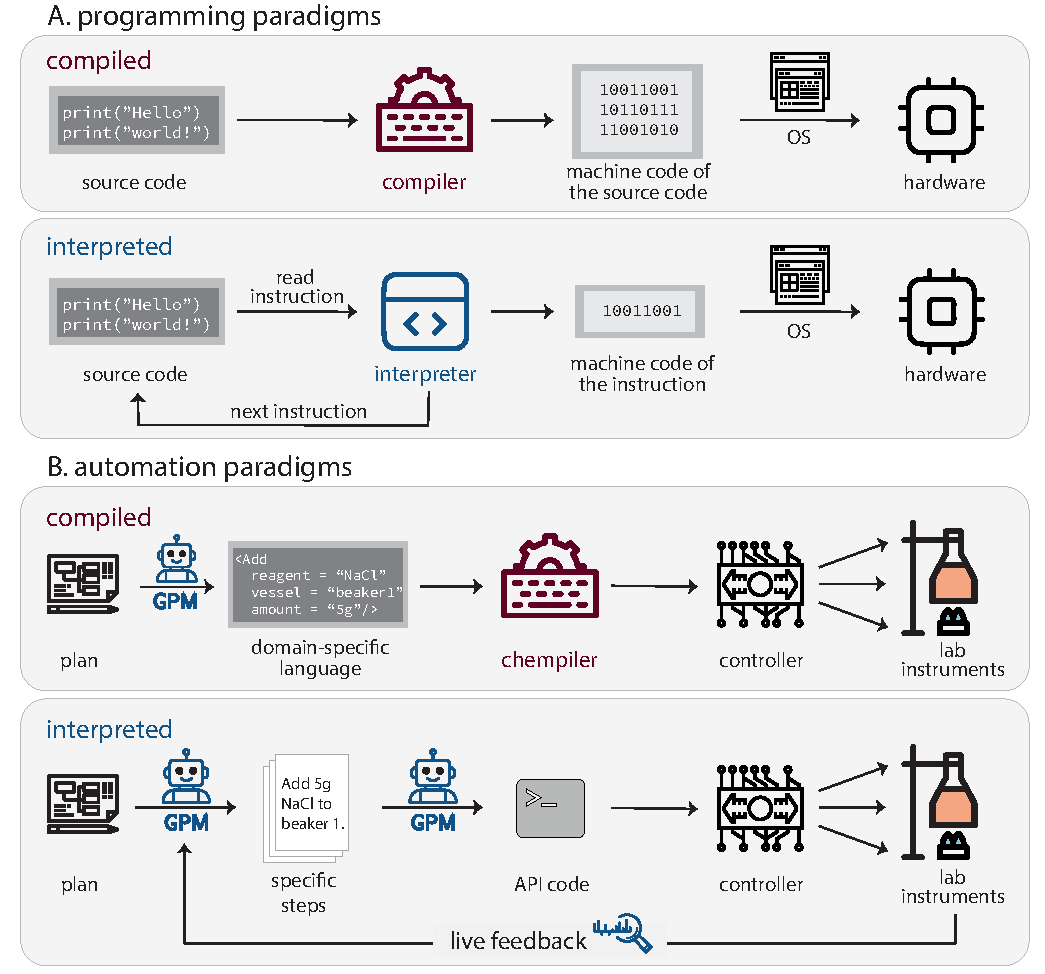
\includegraphics[width=\textwidth]{figures/rescaled_figures/chemrev_figure15+16.pdf}
    \caption{\textbf{Programming languages vs.\ lab automation. A) programming paradigms}: In compiled languages, the entire source code is translated ahead of time to machine code by the compiler. This stand-alone code is then given to the \gls{os}, which is responsible for scheduling and distributing tasks to the hardware. In interpreted languages, the interpreter reads and translates each line of the source code to machine code and hands it to the \gls{os} for execution. \textbf{B) automation paradigms}: In the compiled approach, a \gls{gpm} formalizes the protocol, a compiler, such as the chempiler\autocite{steiner2019organic}, translates the formalized protocol to hardware-specific low-level steps, which the controller then executes---a central hub tasked with scheduling and distributing commands to chemical hardware. In the interpreted approach, a \gls{gpm}, acting as the interpreter, first breaks down the protocol into specific steps, then sends them (via an \gls{api}) for execution one by one. The strength of interpreted systems is dynamic feedback: after the execution of each step, the \gls{gpm} receives a signal (e.g., data, errors), which can influence its behavior for the next steps.}
    \label{fig:exec}
\end{figure}

\subsubsection{Compiled Automation}
In the case of \enquote{compiled automation}, the experiment protocol needs to be formalized in a high-level or \gls{dsl} that describes exactly what operations to perform in what order. 
A chemical compiler (or \enquote{chempiler} \autocite{steiner2019organic}) then converts this high-level protocol into low-level code for the specific lab hardware, which is then executed by robotic instruments, orchestrated by a controller (refer to the caption of \Cref{fig:exec}B). 

\paragraph{Protocol Languages} While \modelname{Python}-based scripts are frequently used as the \textit{de facto} protocol language due to \modelname{Python}'s accessibility and flexibility,\autocite{pylabrobot,vriza2023polybot, wang2025polybot} specialized languages (\glspl{dsl}) have also been developed to provide more structured and semantically rich representations of experimental procedures.\autocite{wang2022ulsa, ananthanarayanan2010biocoder, autoprotocol2023, Park2023CMDL} 
One of the prominent examples of such languages is \gls{chidl}\autocite{xdl2023spec}, developed as part of the Chemputer architecture \autocite{steiner2019organic, mehr2020universal, hammer2021chemputation}. 
\gls{chidl} uses a \gls{json}-like format, and the experimental protocol is described by defining \modelname{Reagents}, \modelname{Vessels}, etc, and using abstract chemical commands such as \modelname{Add}, \modelname{Stir}, \modelname{Filter}, etc. 
In the next step, the \modelname{Chempiler} software takes this \gls{chidl} script and a description of the physical connectivity and composition of the automated platform as a graph and translates it into \gls{chasm} which is specific to the platform (akin to machine code). 
In practice, \gls{chidl}  has been used to automate multi-step organic syntheses with yields comparable to manual experiments.\autocite{mehr2020universal}  

Developing experimental protocols in a formal language is a non-trivial task, often requiring specialized coding expertise. 
Within the compiled approach, the role of the \gls{gpm} is to translate natural-language protocols into their formalized, machine-readable counterparts.\autocite{Lamas2024DSLXpert, jiang2024protocode, conrad2025lowering, inagaki2023robotic} \textcite{Vaucher2020AutoExtraction} used an encoder-decoder transformer model to convert English experimental procedures to structured sequences of pre-defined synthesis actions (e.g., \modelname{MakeSolution}, \modelname{SetTemperature}, \modelname{Extract}). They pre-trained the model on $2$M sentence-action pairs extracted by a rule-based \gls{nlp} algorithm and then fine-tuned it on manually annotated samples to improve accuracy. 
The model achieved exact sentence-pair matching in $61\%$ of the test samples and had more than $75\%$ overlap in $82\%$ of them. 
Although this approach accelerates automated protocol extraction from chemical literature, the output format is not directly suitable for execution. 

\textcite{Pagel2024LLMChemputer} introduced a multi-agent workflow (based on \modelname{GPT-4}) that can address this issue and convert unstructured chemistry papers into executable code. 
The first agent extracts all synthesis-relevant text, including supporting information; a procedure agent then sanitizes the data and tries to fill the gaps from chemical databases (using \gls{rag}); another agent translates procedures into \gls{chidl} and simulates them on virtual hardware; finally, a critique agent cross-checks the translation and fixes errors.

The example above shows one of the strengths of the compiled approach: it allows for pre-validation. 
The protocol can be simulated or checked for any errors before running on the actual hardware, ensuring safety. 
Another example of \gls{llm}-based validators for chemistry protocols is \modelname{CLAIRify}.\autocite{Yoshikawa2023CLAIRify} 
Leveraging an iterative prompting strategy, it uses \modelname{GPT‑3.5} to first translate the natural-language protocol into \gls{chidl} script, then automatically verifies its syntax and structure, identifies any errors, appends those errors to the prompt, and prompts the \gls{llm} again---iterating this process until a valid \gls{chidl} script is produced. 

Similar to how compiled software can be recompiled for different platforms, compiled automation is hardware-agnostic: by using appropriate compilation, a well-defined protocol can---at least in principle---be run on different robotic systems as long as they have the required capabilities.\autocite{rauschen2024universal, strieth-kalthoff2024delocalized,wilbraham2021chemPU} 
In practice, however, inconsistencies in hardware interfaces and software standards across the lab automation community make cross-platform execution challenging.

The main limitations of compiled approaches are the flip side of their strengths: low flexibility and adaptability. 
Any logic or decision-making must either be explicitly encoded within the protocol---necessitating meticulous scripting---or delegated to an external control layer.\autocite{mehr2023digitizing,leonov2024integrated} 
If something unexpected occurs (a pump clogging, a reaction taking longer than expected), the pre-compiled protocol cannot easily adjust in real-time, and human intervention or a complete recompile might be needed.

\subsubsection{Interpreted Automation}
Interpreted programming languages support higher levels of abstraction, enabling the use of more general and flexible command structures. 
Similarly, since \glspl{gpm} can translate high-level goals into concrete steps\autocite{ahn2022can, huang2022language}, they can act as an \enquote{interpreter} between the experimental intent and lab hardware. 
For instance, given an instruction \enquote{titrate the solution until it turns purple}, a \gls{gpm} agent (see \Cref{sec:agents}) can break it down into smaller steps and convert each step to executable code, allowing it to perform incremental additions of titrant and read a color sensor, looping until the condition is met. 
This conversion of concrete steps to code happens at runtime; it is not pre-compiled. 
We refer to such systems as \enquote{interpreted automation} systems. 
In contrast to the deterministic, preplanned nature of compiled systems, interpreted architectures introduce real-time decision-making.
As each action completes, the system collects sensor data (instrument readings, spectra, error messages, etc.) which the agent analyzes and decides on the next action. This allows for dynamic branching and conditional logic during the experiment execution. 

\modelname{Coscientist} \autocite{boiko2023autonomous} is an \gls{llm}-based chemistry assistant built around \modelname{GPT-4} that can autonomously design and execute experiments. 
It can take high-level goals and call tools to write code in real-time in order to control an Opentrons OT-2 liquid-handling robot. The architecture included a web-search module, a documentation module (to read instrument manuals), a \modelname{Python} execution module (to run generated code in a sandbox), and an experiment execution module that sends code to actual lab equipment.
If an error occurred, the system would get feedback and \modelname{GPT-4} would debug its own code. \modelname{Coscientist} successfully planned and executed multistep syntheses with minimal human intervention. 
For example, it efficiently optimized a palladium cross-coupling reaction with minimal human input, outperforming a standard Bayesian optimizer baseline in finding high-yield conditions.

Another example is \modelname{ChemCrow} \autocite{bran2024augmenting}, a \modelname{GPT-4}-based agent augmented with $18$ expert-designed tools for tasks like compound lookup, spectral analysis, and retrosynthesis. \modelname{ChemCrow} can perform tasks across synthesis planning, drug discovery, and materials design by invoking external software for things like retrosynthesis, property prediction, database queries, etc. 
It planned and executed the syntheses of an insect repellent, \gls{deet}, and three different organocatalysts and even guided the discovery of a new chromophore dye. 

The interpreted paradigm is highly generalizable; in principle, the same \gls{llm} agent controlling a chemistry experiment could be re-purposed to a biology or materials experiment with minimal reprogramming because it operates at the level of intent and semantic understanding. 
However, fully autonomous labs featuring interpreted automation are still experimental themselves---ensuring their reliability and accuracy remains an open challenge. 

Despite being labeled as \enquote{autonomous,} both systems mentioned above often need prompting nudges and human correction. 
In addition, these models can replicate known procedures and use databases, but they lack an understanding of mechanisms or underlying principles. Another issue is full reproducibility and long-term experiment tracking. Since the \gls{gpm}'s response might not be deterministic, small changes in prompts can yield different results and closed-source models like \modelname{GPT-4} can change over time. 
Hallucinations remain a risk, especially in planning complex or sensitive reactions. 
In addition, allowing an agent to control hardware brings safety considerations; the flexibility of \glspl{gpm} means that they can devise unanticipated actions. Designing safety nets for these systems is an active area of research. (see \Cref{sec:safety})

\subsubsection{Hybrid Approaches}
Between the two extremes of fully compiled vs.\ fully interpreted automation lies a hybrid approach that seeks to combine the best of both paradigms: the safety and reliability of compiled protocols and the \gls{ai}-driven flexibility of interpreted systems. 

The key difference from purely interpreted systems is that during each experiment run, the plan is fixed, ensuring safety and reproducibility, but between runs, the plan can dynamically change based on the \gls{gpm}’s interpretation of results. 
Once the initial plan (ideally devised by the same \gls{gpm} in a previous step) is provided to a hybrid system, instead of reducing it to smaller steps and directly sending the instructions to a laboratory one at a time, the protocol is first formalized---i.e., it is translated to a formal machine-readable format such as \gls{chidl}. Once validated, the formalized protocol is compiled and executed. After the completion of execution, the \gls{gpm} receives the results and decides what experiment to perform next. This cycle repeats, creating an autonomous optimization or discovery loop. 

This hybrid strategy is attractive because it provides a safety net against mistakes made by the \gls{gpm} interpreter; any generated procedure must pass through a formalization and verification stage before real execution, and therefore, erroneous or hallucinated steps can be caught. For example, if the interpreter hallucinated adding \SI{1000}{\milli\liter} of a solvent but the hardware has only \SI{100}{\milli\liter} capacity, it can be flagged as an error. 



\modelname{ORGANA} \autocite{darvish2025organa} is an \gls{llm}-based robotic assistant following this hybrid paradigm. 
It allows human chemists to describe their experimental goal in natural language. The system can converse with the user to clarify ambiguous requests (the agent would ask \enquote{do you mean X or Y?} if the instructions are unclear). Once the goal is understood, it uses \modelname{CLAIRify} \autocite{Yoshikawa2023CLAIRify} to convert and validate the natural-language description of a chemistry experiment into a \gls{chidl} script, which can be executed on a compatible platform. 
In one case, \modelname{ORGANA} carried out a multistep electrochemistry procedure---polishing electrodes, running an experiment, and analyzing the data---involving 19 substeps that it coordinated in parallel. 
If an unexpected observation occurred (e.g., a solution does not change color when expected), the system can notice via image analysis and modify the plan or alert the user. 
In user studies, \modelname{ORGANA} significantly reduced the manual labor and frustration for chemists, who could offload tedious tasks and trust the agent to handle low-level decisions.

\subsubsection{Comparison and Outlook}
While compiled paradigms continue to provide the backbone for reliable automation, interpreted paradigms will drive exploratory research, where adaptability is key. 
Hybrid systems are likely to be the bridge that brings \gls{ai} into mainstream lab operations, ensuring that flexibility comes with accountability. A brief comparison of the three mentioned approaches is given in \Cref{tab:execution_comparison}.

\begin{table}[ht]
\centering
\caption{\textbf{Comparison of the Compiled, Interpreted, and Hybrid Automation Paradigms}. Each approach has its strengths and weaknesses. Compiled systems favor reliability, interpreted systems allow for more flexibility, while hybrid systems try to strike a balance. }
\begin{tabular}{lccc}
\toprule
\textbf{Feature} & \textbf{Compiled} & \textbf{Interpreted} & \textbf{Hybrid} \\
\midrule
Flexibility & \textcolor{NegativeColor}{Low} & \textcolor{PositiveColor}{High} & Medium \\
Adaptivity & \textcolor{NegativeColor}{None} & \textcolor{PositiveColor}{Real-time} & Iterative \\
Reproducibility & \textcolor{PositiveColor}{High} & Medium & \textcolor{PositiveColor}{High} \\
Safety & \textcolor{PositiveColor}{High} & \textcolor{NegativeColor}{Low} & Medium \\
Setup Overhead & Medium & \textcolor{NegativeColor}{High} & \textcolor{NegativeColor}{High} \\
Industrial Readiness & \textcolor{NegativeColor}{Low} & \textcolor{NegativeColor}{Low} & \textcolor{NegativeColor}{Low} \\
\bottomrule
\end{tabular}
\label{tab:execution_comparison}
\end{table}

While we are essentially witnessing the rise of self-driving laboratories, autonomous experimentation systems present a range of challenges.\autocite{Tom2024SDL,Seifrid2022SDL} 
First, translating high-level natural-language goals into precise laboratory actions remains difficult, as \glspl{gpm} can misinterpret ambiguous instructions, leading to invalid or unsafe procedures. 
This problem is compounded by the lack of universally adopted standards for protocol formalization; while languages like \gls{chidl} show promise, inconsistencies in abstraction, device compatibility, and community uptake limit interoperability. 
Real-time execution adds further complexity, as systems must detect and respond to failures or unexpected behaviors; however, general-purpose validation mechanisms and recovery strategies remain underdeveloped. 
Hardware integration is another bottleneck; current commercial robotic platforms are prohibitively expensive and lab environments often rely on a patchwork of instruments with proprietary interfaces, and building robust, unified control layers demands considerable engineering overhead. 
Another challenge is multi-modality in chemistry; chemists use a wide variety of data (e.g., spectra, TLC plates, SEM images). 
Without integrating these forms of output, models will be limited in their decision-making. 
Finally, ensuring reproducibility and regulatory compliance requires that every step be logged, validated, and traceable at the level required for clinical or industrial adoption (see \Cref{sec:safety}. These challenges must be addressed in tandem to move from experimental demonstrations toward reliable, scalable, and trustworthy autonomous laboratories.


\subsection{Data Analysis}
The analysis of spectroscopic and experimental data in chemistry remains a predominantly manual process. 
Even seemingly straightforward steps, such as plotting or summarizing results, demand repeated manual intervention.

One key challenge that makes automation particularly difficult is the extreme heterogeneity of chemical data sources. 
Laboratories often rely on a wide variety of instruments, some of which are decades old, rarely standardized, or unique in configuration.\autocite{jablonka2022making} 
These devices output data in incompatible, non-standardized, or poorly documented formats, each requiring specialized processing pipelines. 
Despite efforts like \modelname{JCAMP-DX} \autocite{McDonald1988standard}, standardization attempts remain scarce and have generally failed to gain widespread use. 
This diversity makes rule-based or hard-coded solutions largely infeasible, as they cannot generalize across the long tail of edge cases and exceptions found in real-world workflows.

However, this exact complexity makes data analysis in chemistry a promising candidate for \glspl{gpm}. 
They are designed to operate flexibly across diverse tasks and formats, relying on implicit knowledge captured from broad training data. 
In other domains, \textcite{narayan2022can} showed that models like \modelname{GPT-3 DaVinci} can already perform classical data processing tasks such as cleaning, transformation, and error detection through prompting alone. \textcite{kayali2023chorus} introduced \modelname{Chorus} that shows that \glspl{llm} can analyze heterogeneous tabular data without task-specific training. 
\modelname{Chorus} demonstrates that by converting tables into a standardized text format and using zero-shot prompting (i.e., prompts with no examples), \glspl{llm} can flexibly analyze tables even when they differ in structure, column names, or data types.

\begin{figure}[!ht]
    \centering
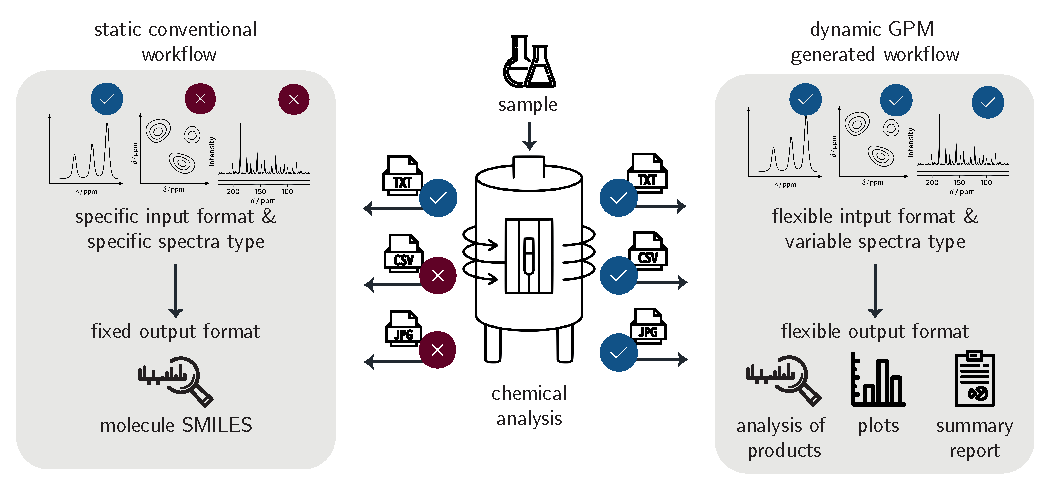
\includegraphics[width=1\textwidth]{figures/rescaled_figures/chemrev_figure17.pdf}
    \caption{\textbf{Static conventional data analysis workflow vs.\ dynamic \gls{gpm} generated workflow}. The chemical analysis can be done with a variety of possible instruments and techniques, resulting in a large number of possible output data formats. The \gls{gpm} can use these diverse, raw data and process it into easy-to-understand plots, analysis and reports. A hard-coded workflow, in contrast, is specifically made to analyze one specific data format and spectra and produces a fixed output format, e.g., the \gls{smiles} of the analyzed molecule.}
    \label{fig:anaylsis}
\end{figure}


 \subsubsection{Prompting} Initial evaluations demonstrated that \glspl{gpm} can support basic data analysis workflows. \autocite{Fu2025large} 
 For example, in chemistry, this enabled the classification of \gls{xps} signals \autocite{decurt2024large} based on peak positions, intensities, or characteristic spectral patterns).  
 
Spectroscopic data are not always available in structured textual form. 
In many practical cases, it appears as raw plots or images, making direct interpretation by \glspl{vlm} a more natural starting point for automated analysis. 
A broad assessment of \gls{vlm}-based spectral analysis was introduced with the \modelname{MaCBench} benchmark \autocite{alampara2024probing}, which systematically evaluates how \glspl{vlm} interpret experimental data in chemistry and materials science---including various types of spectra such as \gls{ir}, \gls{nmr}, and \gls{xrd}q---directly from images. They showed that while \glspl{vlm} can correctly extract isolated features from plots, the performance substantially drops in tasks requiring deeper spatial reasoning.
To overcome these limitations, \textcite{kawchak2024high} explored two-step pipelines that decouple visual perception from chemical reasoning. First, the model interprets each spectrum individually (e.g., converting  \gls{ir}, \gls{nmr}, or \gls{ms} images into textual peak descriptions), and second, a \gls{llm} analyzes these outputs to propose a molecular structure based on the molecular formula. 

\subsubsection{Agentic Systems}
Beyond zero-shot prompting of \glspl{gpm}, one can develop agentic systems that combine multiple analysis steps end-to-end. 
In this regard, \textcite{ghareeb2025robin0} developed \modelname{Robin}---a multi-agent system for assisting biological research with hypothesis generation (see \Cref{fig:hypothesis-generation}) and experimental analysis. 
The data analysis agent \modelname{Finch} performs autonomous analysis of raw or preprocessed experimental data, such as \gls{rna} sequencing and flow cytometry. 
Given a user prompt (e.g., \enquote{\gls{rna} sequencing differential expression analysis}), \modelname{Finch} executes code in a Jupyter notebook to process the data, apply relevant statistical methods, and generate interpretable outputs. For flow cytometry, this includes gating strategies and significance testing, while for \gls{rna} sequencing, it encompasses differential expression and gene ontology enrichment analysis. 
Currently, only these two data types are supported, and expert-designed prompts are still required to ensure reliable results. 

Recent work extends agentic systems beyond single-step data evaluation toward executing and optimizing entire workflows. \textcite{mandal2024autonomous} introduced \modelname{AILA} (Artificially Intelligent
Lab Assistant) utilizing \gls{llm}-agents to plan, code, execute, and revise complete \gls{afm} analysis pipelines. 
The system handles tasks such as image processing, defect detection, clustering, and extraction of physical parameters. 
Compared to systems like \modelname{Finch}, \modelname{AILA} shifts the focus from generating summaries to performing and improving full experimental analyses with minimal user input while maintaining transparency and reproducibility through code and reports.

\subsubsection{Current Limitations}
While \glspl{gpm} offer promising capabilities for automating scientific data analysis, several limitations remain. 
Recent evaluations such as \modelname{FMs4Code} \autocite{tian2024scicode} have shown that even state-of-the-art models like \modelname{GPT-4-Turbo} and \modelname{Claude 2} frequently produce syntactically correct but semantically incorrect code when tasked with common data analysis steps, such as reading files, applying filters, or generating plots. 
Typical issues include incorrect column usage, or inconsistent output formatting.

These technical shortcomings are reinforced by the model's sensitivity to prompt formulation. As demonstrated by \textcite{Yan2020auto} and \textcite{alampara2024probing}, minor changes in wording or structure can lead to significantly different outputs, highlighting a lack of robustness in prompt-based control. 

Together, these findings suggest that while foundation models can generalize across diverse data formats and analysis types, their current performance is not yet sufficient for fully autonomous use in scientific analysis settings. 
Robust prompting strategies, post-generation validation, and human oversight remain essential components in practice.



\subsection{Reporting}
To share insights obtained from data analysis, one often converts them into scientific reports. 
Also, in this step, \glspl{gpm} can take a central role, which we discuss in the following.

Reporting refers to converting scientific results into shareable reports, scientific publications, blogs, and other forms of content. 
This section describes two main applications of \glspl{llm} in scientific reporting: converting data into explanations and the first steps towards using these models as fully-fledged writing assistants.

\subsubsection{From Data to Explanation}

The lack of explainability of \gls{ml} predictions generates skepticism among experimental chemists\autocite{wellawatte2025human}, hindering the wider adoption of such models.\autocite{wellawatte2022model}
One promising approach to address this challenge is to convey explanations of model predictions in natural language. 
An approach proposed by \textcite{wellawatte2025human} is to couple \glspl{llm} with feature importance analysis tools, such as \gls{shap} or \gls{lime}. 
In this framework, \glspl{llm} can additionally interact with tools such as \gls{rag} over \modelname{arxiv} to provide evidence-based explanations.

\subsubsection{Writing Assistance} When considering \gls{ml}-based assistance in scientific writing, we can distinguish two primary modes: systems that aid authors during the active writing process and tools that optimize or refine scientific articles after initial drafting.

The former refers to the use of writing copilots that can suggest syntax improvement, identify text redundancies,\autocite{khalifa2024using} caption figures and tables\autocite{hsu2021scicap,selivanov2023medical}, or provide caption-figure match evaluation\autocite{hsu2023gpt04}, but also more specific applications like writing alt-text (descriptive text that explains the meaning and purpose of an image in digital content)\autocite{singh2024figura11y}. 

Under the latter mode, \gls{gpm} can be used to assist non-native English speakers with scientific writing \autocite{giglio2023use}.
It could even allow authors to write in their native language and use \gls{gpm} for communicating scientific results in English.

Another application of \gls{llm} is to assist with completing checklists before submitting a publication. For example, \textcite{goldberg2024usefulness} benchmark the use of \glspl{llm} in completing the author checklist for the \gls{neurips} 2025. They concluded that $70\%$ of the authors found the \gls{llm}-assistant useful, with the same fraction indicating they would revise their own checklist based on the model feedback.




\subsubsection{Vision} 

Few have ventured into fully automating the writing process.\autocite{yamada2025ai} 
While at its inception, reporting using \gls{gpm} has tremendous potential. 
In \Cref{fig:writing_with_ml} we showcase how the future of reporting could look like if we were to integrate \gls{gpm} at each step of the process.

\begin{figure}[!ht]
    \centering
        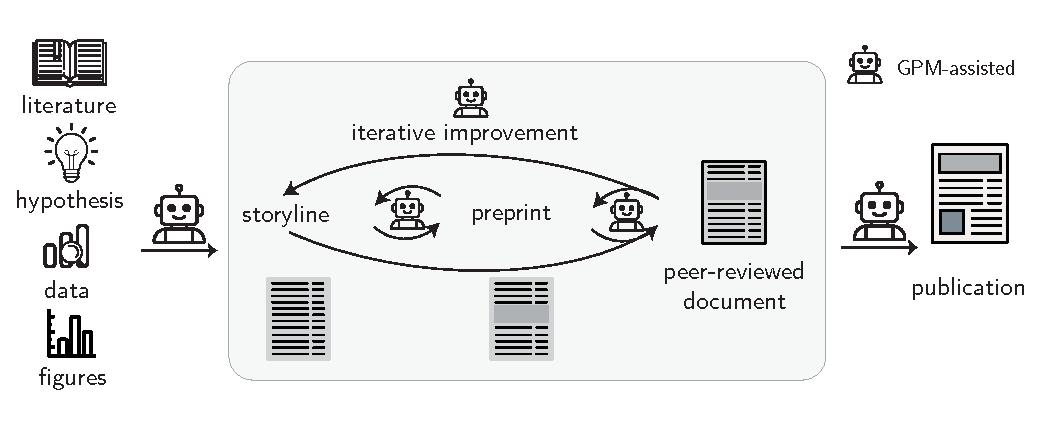
\includegraphics[width=1\textwidth]{figures/rescaled_figures/chemrev_figure18.pdf}
    \caption{\textbf{Vision for \gls{gpm} in reporting, a visualization of the scientific writing process}. \glspl{gpm} can be used at every stage of the process. For creating the pre-print, we can utilize the multimodal capabilities of these models to write detailed captions for figures. For the peer-review process, we can harness the ability of \glspl{gpm} to summarize and prioritize information (e.g., design a time-efficient plan to address the peer review). When converting a document from a peer-reviewed pre-print, we often need to implement the publisher's requirements. In this case, we can make use of agentic systems that would assist with minor text fixes or document restructuring.}
    \label{fig:writing_with_ml}
\end{figure}

An idea entertained by \textcite{li2023teach} in the context of education is personalized writing. 
However, it is still widely unexplored in its goal: to make science accessible to everyone. 
A personalized model that learns user preferences and domain expertise can be used to deliver the message of a scientific article in simpler terms. 
As a result, we might observe a rise in cross-domain scientific collaborations and a rising interest in science. 

\section{Accelerating Applications}
The application of accelerated approaches in the scientific discovery cycle (see \Cref{fig:applications}) hinges on their ability to streamline and enhance each stage of the process.
However, a fundamental challenge in effectively implementing these approaches lies in the choice of machine-readable representation.

This challenge is particularly evident in the representation of molecules and materials, which must balance computational efficiency with the preservation of structural, compositional, and functional properties. 
Take, for example, the high-temperature superconductor \ce{YBa2Cu3O_{7-x}}. 
While atomic positions and coordinates are theoretically sufficient to solve the Schrödinger equation and describe this material, such a representation may not provide the adaptability necessary for diverse tasks. What defines a good representation depends on the problem. \autocite{huang2016understanding}. 
A representation designed to predict critical temperature must efficiently encode the relationship between oxygen stoichiometry and superconducting properties, emphasizing features like oxygen vacancy patterns and charge transfer mechanisms. 
Conversely, a representation for structural stability might prioritize different geometric or bonding characteristics.

This tension has led to three primary strategies for representing molecules and materials (read \Cref{sec:common_representations} to learn in detail about the different representations that currently exist). 
First, domain-specific text-based formats---such as \gls{smiles} \autocite{weininger1988smiles}, \gls{selfies} \autocite{krenn2020self}, and \gls{cif} \autocite{hall1991crystallographic}---offer compact, machine-readable encodings of structural information. While these necessarily omit certain physical details, their computational tractability has enabled breakthroughs, as demonstrated by \textcite{jablonka2024leveraging} in their \gls{llm}-based generation of valid molecular and material structures.

Yet, the question remains: Which representation is optimal for a given task? Future advances in accelerated discovery will likely hinge on adaptive representations that dynamically balance these competing demands.

\subsection{Property Prediction} \label{sec:prediction}

\glspl{gpm} have emerged as a powerful tool for predicting molecular and material properties, offering an alternative to traditional quantum mechanical calculations or specialized \gls{ml} models. 
Current \gls{gpm}-driven property prediction tasks span both classification and regression. 
Unlike conventional approaches that rely on task-specific architectures and extensively labeled data, \glspl{gpm} have demonstrated strong generalization capabilities across diverse domains, efficiently adapting to various prediction tasks. 
Their success extends to multiple datasets, from standardized benchmarks such as \modelname{MoleculeNet} \autocite{wu2018moleculenet}, to curated datasets targeting specific applications such as antibacterial activity \autocite{chithrananda2020chemberta} or photovoltaic efficiency\autocite{aneesh2025semantic}.

Three key methodologies have been explored to adapt \glspl{llm} for property prediction: prompting techniques (see \Cref{sec:prompting}), fine-tuning (see \Cref{sec:fine-tuning}) on domain-specific data, and \gls{rag} (see \Cref{sec:rag}) approaches that combine \glspl{llm} with external knowledge bases. 

\begin{table}[htbp]
    \centering
    \caption{\textbf{Non-comprehensive list of \glspl{gpm} applied to property prediction tasks}. The table presents different models and their applications across different molecular and materials property prediction benchmarks, showing the diversity of properties (from molecular toxicology to crystal band gaps), datasets used for evaluation, modeling approaches (prompting, fine-tuning, or retrieval-augmented generation), and task types (classification or regression.)}
    \label{tab:property_prediction_models}
    \resizebox{\textwidth}{!}{%
    \begin{tabular}{lllcc}
        \toprule
        \textbf{Model} & \textbf{Property} & \textbf{Dataset} & \textbf{Approach}  & \textbf{Task}\\
        \midrule
        \multirow{7}{*}{GPT-Chem\autocite{jablonka2024leveraging}} & HOMO/LUMO & QMUGs\autocite{isert_qmugs_2022} & \multirow{7}{*}{FT} & C, R \\
        & Solubility & DLS-100\autocite{mitchell_dls-100_2017} & & C, R \\
        & Lipophilicity & LipoData\autocite{jablonka2024leveraging} & & C, R \\
        & Hydration Free Energy & FreeSolv\autocite{mobley_freesolv_2014} & & C, R \\
        & Photoconversion Efficiency & OPV\autocite{jablonka2024leveraging} & & C, R  \\
        & Toxicology & Tox21\autocite{richard_tox21_2021} & & C, R  \\
        & $\text{CO}_2$ Henry Coefficients of MOFs & MOFSorb-H\autocite{lin_silico_2012} & & C, R \\
        \cmidrule{1-5}
        \multirow{3}{*}{LLM-Prop\autocite{rubungo_llm-prop_2023}} & Band Gap & \multirow{3}{*}{CrystalFeatures-MP2022\autocite{rubungo_llm-prop_2023}} & \multirow{3}{*}{P} &  R  \\
        & Volume & & & R \\
        & Is the band gap direct?&  & & C \\
        \midrule
        \multirow{12}{*}{LLM4SD\autocite{zheng2025large}} & Blood-brain barrier penetration & BBBP\autocite{sakiyama_prediction_2021} & \multirow{10}{*}{P} & C \\
        & FDA approval & ClinTox\autocite{wu2018moleculenet} & & C \\
        & Toxicology & Tox21\autocite{richard_tox21_2021} & & C \\
        & Drug-related side effects & SIDER\autocite{kuhn_sider_2016} & & C \\
        & HIV replication inhibition & HIV\autocite{wu2018moleculenet} & & C \\
        & $\beta$-secretase binding & BACE\autocite{wu2018moleculenet} & & C \\
        & Solubility & ESOL\autocite{wu2018moleculenet} & & R \\
        & Hydration Free Energy & FreeSolv\autocite{mobley_freesolv_2014} & & R \\
        & Lipophilicity & Lipophilicity\autocite{wu2018moleculenet} & & R \\
        & Quantum Mechanics & QM9\autocite{wu2018moleculenet} & & R \\
        \midrule
        \multirow{4}{*}{\modelname{LLaMP\autocite{chiang2024llamp}}} & Bulk modulus & \multirow{4}{*}{Materials Project\autocite{riebesell2025framework}} & \multirow{4}{*}{RAG} & R \\
        & Formation energy & & & R \\
        & Electronic bandgap & & & R \\
        & Multi-element electronic bandgap & & & R \\
        \bottomrule
    \end{tabular}
    }
    \vspace{0.5em}
    \footnotesize
    \begin{minipage}{\linewidth}
        \textbf{Key:}  P = prompting; FT = fine-tuned model; RAG = retrieval-augmented generation; C = Classification; R = Regression
    \end{minipage}
\end{table}

\subsubsection{Prompting} 
Prompt engineering involves designing targeted instructions to guide \glspl{gpm} in performing specialized tasks without altering their underlying parameters by leveraging their embedded knowledge. 
In molecular and materials science, this strategy goes beyond simply asking a model to predict properties. 
It also includes carefully structured prompts to elicit detailed molecular and material descriptions directly from the model's pre-trained knowledge.

\textcite{liu2025integrating} conducted a comprehensive evaluation of different prompting techniques to predict the properties of organic small molecules and crystal materials. 
Some of these techniques included domain-knowledge (prior knowledge was embedded in the prompt), expert (role-play instructions), and few-shot \gls{cot} (the text\textit{\enquote{Let's think step by step}} is added) prompting. 
Of these, domain knowledge achieved maximum performance. However, their evaluation was limited to a relatively small set of molecules and tasks, and the effectiveness of their domain-knowledge approach may not generalize to other molecular property domains.

Building on these foundational prompting strategies, few-shot prompting approaches leverage \gls{icl} to enhance performance through selected examples \textcite{liu2024moleculargpt} used \gls{smiles} string representations of molecules with few-shot \gls{icl}, retrieving structurally similar molecules as demonstrations to enhance property prediction. 
This approach highlights how \gls{icl} can transfer knowledge from similar molecule examples without requiring model fine-tuning for each task. 
However, the effectiveness of \gls{icl} depends on the quality of retrieved examples.

\textcite{fifty2023incontext} moved beyond direct text prompting of molecules and introduced \gls{camp}: an \gls{icl} algorithm that uses a two-stage encoding approach without relying on pre-trained \glspl{llm}.
First, a specialized \gls{mpnn} encodes molecule graphs into molecular embeddings rather than processing them as raw text. 
These embeddings are then fed into a transformer encoder, which learns contextualized representations across the support set (a small collection of labeled molecule-property pairs) and the unlabeled query molecules. They demonstrated \gls{camp}'s ability to outperform existing few-shot learning baselines by providing relevant molecular examples within the prompt context. However, this approach is constrained by the context-length limitations of the underlying \glspl{lm} and the challenge of selecting optimal demonstration examples.

More sophisticated approaches have leveraged prompting as part of multi-modal frameworks. The \modelname{LLM4SD} pipeline by \textcite{zheng2025large} employs specialized prompts to guide \glspl{lm} through their pre-trained knowledge on scientific literature, generating known rules (e.g., molecules weighing under \SI{500}{Da} are more likely to pass the blood-brain barrier) that transform molecules into feature vectors (e.g. \ce{CCO} could translate to a vector $[2,46.07,1,1]$ where each number represents a feature of the molecule, in this example [\# \ce{C}, MW, \# \ce{H}-bond donors, \# \ce{H}-bond acceptors]) for use with a random forest model, which they consider \enquote{interpretable}. 
This approach outperformed specialized \gls{sota} models across $58$ benchmark tasks, while providing interpretable reasoning about prediction logic (see \Cref{tab:property_prediction_models} for properties predicted by this model). However, its reliance on rule extraction may limit its ability to capture complex, non-linear relationships that specialized deep learning models can identify.

\paragraph{\glspl{llm} as Feature Extractors} Another emerging application of \glspl{llm} is their use as \enquote{feature extractors}, where they generate textual or embedded representations of molecules or materials. For instance, in materials science, \textcite{aneesh2025semantic} employed \glspl{llm} to generate text embeddings of perovskite solar cell compositions. 
These embeddings were subsequently used to train a \gls{gnn} for predicting power conversion efficiency, demonstrating the potential of \glspl{llm} to enhance feature representation in materials informatics. 
Similarly, in the molecular domain, \textcite{srinivas2024crossmodal} used zero-shot \gls{llm} prompting (see \Cref{box: cot_prompting} for prompt examples) to generate detailed textual descriptions of molecular functional groups, which are used to train a small \gls{lm}. This \gls{lm} is used to compute text-level embeddings of molecules. Simultaneously, they generate molecular graph-level embeddings from \gls{smiles} string molecular graph inputs. They finally integrate the graph and text-level embeddings to produce a semantically enriched embedding.
\begin{promptbox}\label{box: cot_prompting}
    \textbf{\gls{cot} Prompting}\autocite{srinivas2024crossmodal}\\
    Prompt 1: What is the molecular structure of this chemical \gls{smiles} string? Could you describe its atoms, bonds, functional groups, and overall arrangement? \\
    Prompt 2: What are the physical properties of this molecule, such as its boiling point and melting point?\\
    ...\\
    Prompt 14: Are there any environmental impacts associated with the production, use, or disposal of this molecule?
\end{promptbox}
In a different implementation of fine-tuning, \textcite{balaji2023gptmolberta} used \modelname{ChatGPT} to generate text descriptions of molecules that were then used to train a \modelname{RoBERTa} (125M) model for property prediction, showing how \gls{lm}-generated representations can access latent spaces that \gls{smiles} strings alone might not capture.
Similarly, \textcite{li2024unveiling} introduced the \modelname{MoleX} framework, which fine-tunes \modelname{ChemBERTa-2}\autocite{ahmad2022chemberta} on Group \gls{selfies} \autocite{cheng2023group} (a functional group-based molecular representation) to then extract a single \gls{llm}-derived embedding of molecules that captures the chemical semantics at the functional group level. This allowed them to determine which functional groups or fragments contribute to molecular properties, which in turn can be converted into reliable explanations of said properties.

\subsubsection{Fine-Tuning}\label{sec:prediction_FT}
\begin{figure}[htb] 
    \centering
    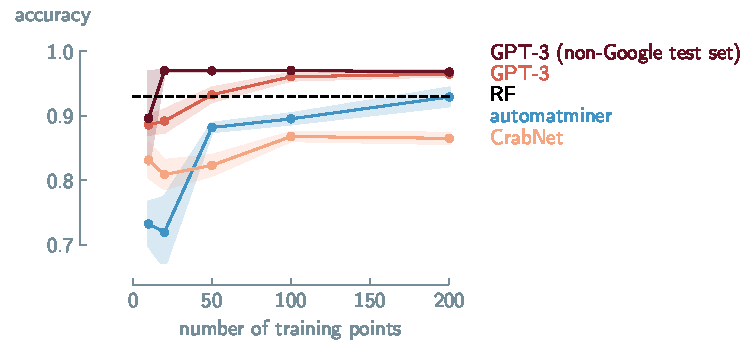
\includegraphics[width=1\textwidth]{figures/property_gptchem.pdf}
    \caption{\textbf{Fine-tuned \modelname{GPT-3} for predicting solid-solution formation in high-entropy alloys} Performance comparison of different \gls{ml} approaches as a function of the number of training points. Results are shown for \modelname{Automatminer} (blue), \modelname{CrabNet} transformer (orange),  fine-tuned \modelname{GPT-3} (red), with error bars showing standard error of the mean. The non-Google test set shows the fine-tuned \modelname{GPT-3} model tested on compounds without an exact Google search match (dark red). The dashed line shows performance using random forest. \modelname{GPT-3} achieves comparable accuracy to traditional approaches with significantly fewer training examples. Data adapted from \textcite{jablonka2024leveraging}}
    \label{fig:gptchem}
\end{figure}

\paragraph{\gls{lift}} \textcite{dinh2022lift} showed that reformulating regression and classification as \gls{qa} tasks enables the use of unmodified model architecture while improving performance (see \Cref{sec:fine-tuning} for a deeper discussion of \gls{lift}). 
In recognizing the scarcity of experimental data and acknowledging the persistence of this limitation, \textcite{jablonka2024leveraging} designed a \gls{lift}-based framework using \modelname{GPT-3} fine-tuned on task-specific small datasets (see \Cref{tab:property_prediction_models}). 
They seminally demonstrated that fine-tuned \modelname{GPT-3} can match or surpass specialized \gls{ml} models in various chemistry tasks. A key finding was fine-tuned \modelname{GPT-3}'s ability to generalize beyond training data. 
When tested on compounds absent from Google Search (and likely its training data), it performed well, proving that it was not simply recalling memorized information (see \Cref{fig:gptchem}).

In a follow-up to \textcite{jablonka2024leveraging}'s work, \textcite{vanherck2025assessment} systematically evaluated this approach across 22 diverse real-world chemistry case studies using three open-source models. They demonstrate that fine-tuned \glspl{llm} can effectively predict various material properties. For example, they achieved $96\%$ accuracy in predicting the adhesive free-energy of polymers, outperforming traditional \gls{ml} methods like random forest ($90\%$ accuracy). When predicting properties of monomers using \gls{smiles} notation, the fine-tuned models reached average accuracies of $84\%$ across four different properties. Particularly notable was the ability of \glspl{llm} to work with non-standard inputs, like in a protein phase separation study they did, where raw protein sequences could be directly input without pre-processing and achieve $95\%$ prediction accuracy. At the same time, when training datasets were very small (15 data points), the predictive accuracy of all fine-tuned models was lower than the random baseline (e.g. MOF synthesis). These case studies preliminarily demonstrate that these models can achieve predictive performance with some small datasets, work with various chemical representations (\gls{smiles}, \gls{mof}id, and \gls{iupac} names), and can outperform traditional \gls{ml} approaches for some material property prediction tasks.

In the materials domain, \modelname{LLMprop} fine-tunes \modelname{T5}\autocite{raffel2020exploring} to predict crystalline material properties from text descriptions generated by \modelname{Robocrystallographer}\autocite{ganose2019robocrystallographer}. By discarding \modelname{T5}’s decoder and adding task-specific prediction heads, the approach reduces computational overhead while leveraging the model’s ability to process structured crystal descriptions. The method demonstrates that natural language representations can effectively capture key material features, offering an alternative to traditional graph-based models like \glspl{gnn}.

Fine-tuning has been used to adapt \glspl{ssm} like Mamba (see \Cref{sec:example_architectures}). By pre-training on 91 million molecules, the Mamba-based model \modelname{$\text{O}_{SMI}-{\text{SSM}-}336\textit{M}$} outperformed transformer methods (\modelname{Yield-BERT}\autocite{krzyzanowski2025exploring}) in reaction yield prediction (e.g., Buchwald-Hartwig cross-coupling) and achieved competitive results in molecular property prediction benchmarks.\autocite{soares2025mamba-based} 

\paragraph{Foundational \glspl{gnn} and \glspl{mlip}} The fine-tuning approach has been applied to \enquote{foundational \glspl{gnn}} \autocite{sypetkowski2024scalability, shoghi2023molecules} and \glspl{mlip}, approaches distinct from \glspl{gpm}. For example, \textcite{shoghi2023molecules, sypetkowski2024scalability} show \gls{sota} performance on property prediction tasks.
\enquote{Foundational} \glspl{mlip} pre-trained on large datasets encompassing many chemical elements can be fine-tuned for specific downstream tasks \autocite{batatia2022mace}, such as calculating sublimation enthalpies of molecular crystal polymorphs \autocite{kaur2025data}.

\paragraph{Limitations} One central challenge is finding balance in datasets. In practical applications, researchers often have many more examples of poor-performing materials than optimal ones, resulting in unbalanced datasets that can diminish model performance. \textcite{vanherck2025assessment} point out that in the catalyzed cleavage reaction study, only $3.8\%$ of catalysts were labeled as \enquote{good}, forcing researchers to reduce their training set significantly to maintain balance. They also note that \glspl{llm} struggle with highly complex or noisy datasets, as seen in their study of catalytic isomerization, where even after hyperparameter optimization, the models failed to achieve meaningful predictive power due to the high noise in the experimental data and limited sample size. Finally, they note that although \glspl{llm} can work with different chemical representations, the choice of representation significantly impacts performance. For example, when predicting polymerization rates, models using \gls{smiles} notation significantly outperformed those using \gls{iupac} names, indicating that representation selection remains an important consideration.

Fine-tuning effectively adapts \glspl{llm} to specialized chemistry tasks, but its dependence on static datasets hinders adaptability to new or evolving knowledge. \gls{rag}, whose fundamentals are described in detail in \Cref{sec:rag}, overcomes these limitations by dynamically integrating external data sources, enabling more flexible and up-to-date reasoning.

\subsubsection{Agents}

Caldas Ramos et al.\ introduce \modelname{MAPI-LLM}, a framework that processes natural-language queries about material properties using an \gls{llm} to decide which of the available tools such as the Materials Project \gls{api}, the Reaction-Network package, or Google Search to use to generate a response. \autocite{Jablonka2023} \modelname{MAPI-LLM} employs a \gls{react} prompt (see \Cref{sec:arch_agents} to read more about \gls{react}), to convert prompts such as  \textit{\enquote{Is $Fe_2O_3$ magnetic?}} or \textit{\enquote{What is the band gap of Mg(Fe3O3)2?}} into queries for Materials Project \gls{api}. 
The system processes multi-step prompts through logical reasoning, for example, when asked \textit{\enquote{If Mn2FeO3 is not metallic, what is its band gap?}}, the \gls{llm} system creates a two-step workflow to first verify metallicity before retrieving the band gap.

Building on this foundation of agent-based materials querying, \textcite{chiang2024llamp} advanced the approach with \modelname{LLaMP}, a framework that employs \enquote{hierarchical} \gls{react} agents to interact with computational and experimental data. This \enquote{hierarchical} framework employs a supervisor-assistant agent architecture where a complex problem is broken down and tasks are delegated to domain-specific agents.  \modelname{LLaMP} addresses the challenge of hallucinations more effectively than standard \gls{llm} approaches by grounding responses in retrieved materials databases, retrieving materials data (e.g., crystal structures, elastic tensors) while counteracting systematic \gls{llm} biases in property predictions. These biases include the tendency for \glspl{llm} to overestimate certain properties like bulk moduli and to exhibit errors in bandgap predictions based on compositional patterns learned during training rather than physical principles.


\subsubsection{Core Limitations}\label{sec:property_core_limits}

\begin{figure}[htb]
    \centering
    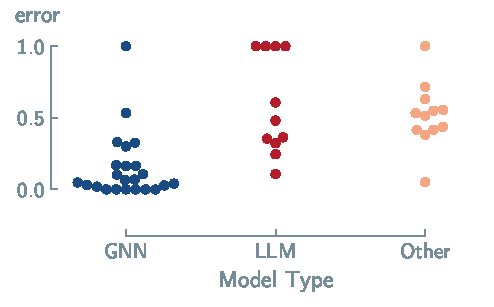
\includegraphics{figures/property_mattext.pdf}
    \caption{\textbf{Normalized error distributions for materials property prediction models across different architectures}. Each point represents the normalized error of a model on a specific property prediction task. Normalization was achieved with min/max values of each dataset to produce a range of errors between 0 and 1. The first column (blue) shows \gls{gnn} based models, the second column (red) displays \gls{llm} approaches, and the third column (orange) represents other baseline methods and \gls{sota} models including \modelname{CrabNet}. \autocite{Wang_2021} Lower values indicate better predictive performance. Data adapted from \textcite{alampara2024mattext}}
    \label{fig:property_limitations}
\end{figure}

\noindent \textcite{alampara2024mattext} introduced \modelname{MatText}, a framework for evaluating \glspl{lm} ability to predict properties of materials using text-based representations. 
Their findings indicate that current \glspl{llm} (including pre-trained \modelname{BERT} and fine-tuned \modelname{LLaMA-3-8B}) are effective for tasks relying purely on compositional information (e.g., element types and local bonding patterns), but struggle to leverage geometric or positional information encoded in text, as reflected in \Cref{fig:property_limitations}. 
This observation suggests that transformer-based architectures may be fundamentally limited to applications where spatial understanding is not required. 
Their experiments with data scaling and text representations reveal that increasing pre-training data or adding geometric details fails to improve downstream property prediction, challenging the conventional assumption that larger models and datasets universally enhance performance. \autocite{frey2023neural} 
Notably, \textcite{frey2023neural} demonstrated power-law scaling in chemical \glspl{llm}, but \modelname{MatText}'s results imply that such scaling may not overcome architectural biases against geometric reasoning in materials tasks.\autocite{gruver2024promises}

\subsection{Molecular and Material Generation} \label{sec:mol_generation}

\begin{figure}[htbp!]
    \centering
    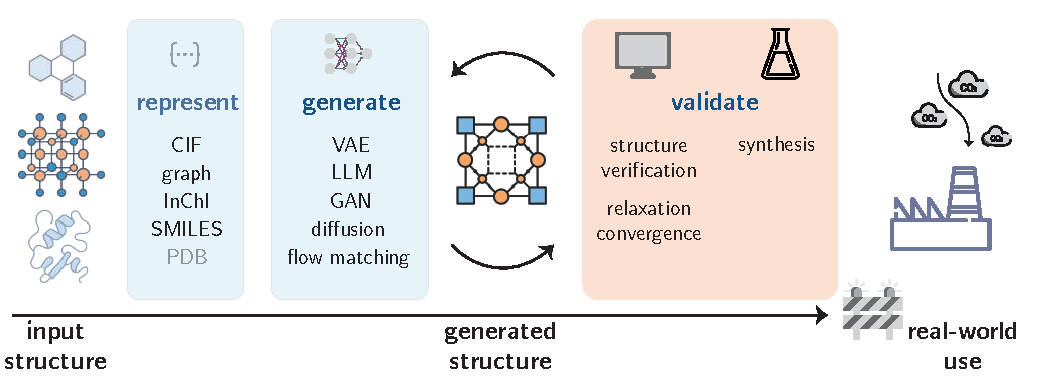
\includegraphics[width=1\textwidth]{figures/rescaled_figures/chemrev_figure21.pdf}
    \caption{\textbf{Pipeline for molecular and materials generation} The workflow begins with input structures represented in various formats, which are used to train \gls{ml} models to generate novel molecular and material structures. The generated structures should undergo a feedback loop through validation processes before being applied in the real world. Blue boxes indicate well-established areas of the pipeline with mature methodologies, while the red box represents critical bottlenecks.}
    \label{fig:generation}
\end{figure}

\noindent Early work in molecular and materials generation relied heavily on unconditional generation, where models produce novel structures without explicit guidance, relying solely on patterns learned from training data. For example, latent space sampling in autoencoders, where random vectors are decoded into new structures.\autocite{yoshikai2024novel} These methods excel at exploring chemical space broadly but lack fine-grained control. 
This limitation underscores the need for conditional generation, using explicit prompts or constraints (e.g., property targets, structural fragments), to steer \glspl{gpm} toward meaningful molecule or material designs. 
Beyond the generation step, as \Cref{fig:generation} shows, critical bottlenecks persist in synthesizability and physical consistency at the validation stage.

\subsubsection{Generation}\label{sec:generation}

\paragraph{Prompting}
While zero-shot and few-shot prompting strategies demonstrate promising flexibility for molecule generation, benchmark studies \autocite{guo2023large} reveal significant limitations that restrict their practical utility. \textcite{guo2023large} exposed fundamental gaps in \glspl{llm}' molecular design capabilities through a systematic evaluation. \modelname{GPT-4} was reported to produce chemically valid \gls{smiles} $89\%$ of the time but achieving less than $20\%$ accuracy in matching the target specifications. 
This result is far below specialized models like \modelname{MolT5}\autocite{edwards2022translation}. 
They conclude that this performance gap stems from \glspl{llm}' inadequate understanding of \gls{smiles} syntax and structure-property relationships. 
Subsequent work by \textcite{bhattacharya2024large} explored whether systematic prompt engineering could overcome these limitations, demonstrating that these prompts could guide \modelname{Claude 3 Opus} to generate chemically valid molecules ($97\%$ syntactic validity) with controlled modifications, including fine-grained structural changes (median Tanimoto similarity $0.67$--$0.69$) and predictable electronic property shifts (\SIrange{0.14}{0.27}{eV} \gls{homo} energy changes). Hybrid approaches like \modelname{FrontierX} extend this method with knowledge-augmented prompting, where \glspl{llm} generate both molecule predictions and explanations that are used to fine-tune smaller \glspl{lm}, with all resulting embeddings ultimately combined via hierarchical attention mechanisms to produce the final \gls{smiles} representation\autocite{srinivas2024crossing}. 
It showed improved accuracy over pure prompting strategies but sacrificed the generalizability that makes \glspl{llm} attractive, as the model requires re-training for each new molecular domain. 

\paragraph{Fine-Tuning} To overcome the limitations of prompting, fine-tuning has been adopted in molecular and materials generation, much like its use in property prediction with \gls{lift}-based frameworks (see \Cref{sec:fine-tuning} for a deeper explanation of \gls{lift} and \Cref{sec:prediction_FT} for a discussion of \gls{lift} applied to property prediction tasks). \textcite{yu2024llasmol} demonstrated that systematic fine-tuning in various chemical tasks including molecule generation from captions can improve performance while remaining parameter-efficient, using only $0.58\%$ of trainable parameters via \gls{lora}.

The molecule-caption translation task (\modelname{Mol2Cap}), which involves generating textual descriptions from molecular representations and vice versa (Cap2Mol), has become a standard benchmark for evaluating \glspl{gpm} for molecule generation. \autocite{edwards2022translation} Under the \enquote{Mol2Cap}/\enquote{Cap2Mol} task paradigm, \gls{icma} avoids domain-specific pre-training by combining retrieval-augmented in-context learning with fine-tuning on \gls{icl} examples.\autocite{li2025large} 
On the ChEBI-20\autocite{edwards2021text2mol} and PubChem324k\autocite{liu2023molca} datasets, \gls{icma} nearly doubles baseline performance, with \gls{icma} powered by\modelname{Mistral-7B} achieving a 0.581 \gls{bleu} score in \modelname{Mol2Cap} and $46.0\%$ exact match in \modelname{Cap2Mol}.\autocite{li2025large} 
However, its reliance on retrieved examples raises concerns about generalization to novel scaffolds. 
Similarly, \modelname{MolReFlect} enhances fine-grained alignment through a teacher-student framework, where a larger \gls{llm} (e.g., \modelname{GPT-4}) extracts substructure-aware captions to guide a smaller model (\modelname{Mistral-7B}), improving \modelname{Cap2Mol} accuracy while reducing hallucinations.\autocite{li2024molreflect} 
Meanwhile, \modelname{PEIT-LLM} extends the task to property-conditioned generation, using instructions (\gls{smiles}-text-property tuples) to optimize for captioning and prediction jointly.\autocite{lin2025property} 

Fine-tuned \glspl{lm} have shown promise in molecule and materials generation. 
However, their reliance on decoding and \gls{smiles}/\gls{selfies} representations introduces fundamental limitations: degeneracy (multiple valid \gls{smiles} for the same molecule) and difficulty capturing complex structural relationships implicit in textual descriptions.

\paragraph{Diffusion and Flow Matching} Diffusion and flow-based models operate directly on latent representations, enabling more flexible generation of diverse and novel structures.\autocite{zhu20243m-diffusion} Moreover, emerging hybrid architectures combine the strengths of \glspl{llm} with diffusion and flow matching models to overcome the limitations of each paradigm individually \autocite{sriram2024flowllm}.

Beyond text-based representations, \modelname{llamole} introduced a multimodal \gls{llm} approach capable of text and graph generation by integrating a base \gls{llm} with graph diffusion transformers and graph neural networks for multi-conditional molecular generation and retrosynthetic planning. Specifically they used different trigger (\texttt{<design>} and \texttt{<retro>}) and query (\texttt{<query>}) tokens for switching between them and improved success in synthesis success rates from  $5\%$ to $35\%$ . \autocite{liu2024multimodal}

A unique challenge with crystalline materials is generating a material that possesses both discrete (atom type) and continuous (atomic position and lattice geometry) variables. \textcite{sriram2024flowllm} developed \modelname{FlowLLM} to address this challenge. They recognized that the respective strengths of \glspl{llm}, modeling discrete values and conditional prompting, and denoising models, modeling continuous values and equivariances, could be combined to create a hybrid architecture. 
A fine-tuned \gls{llm} is used to learn an effective base distribution of metastable crystals via text-based representations, which is then iteratively refined through \gls{rfm} to optimize atomic coordinates and lattice parameters.\autocite{sriram2024flowllm}

\paragraph{Reinforcement Learning and Preference Optimization}

Translating \gls{gpm} generated outputs to the real world requires designing molecules and materials with specific target properties. \gls{rl} and preference optimization techniques\autocite{lee2024fine-tuning} have emerged as powerful solutions for this challenge. For instance, \textcite{jang2025can} combined \gls{sft} and \gls{rl} using \gls{ppo} to generate diverse molecular sequences auto-regressively. 
This approach excels in exploring a broad chemical space, but incurs high computational costs due to its reliance on iterative, sequence-based generation. 
In contrast, \textcite{cavanagh2024smileyllama} employed \gls{dpo} with \gls{sft} to fine-tune \glspl{llm} for molecular design, leveraging \gls{smiles} representations to optimize drug-like properties (e.g., hydrogen bond donors/acceptors and LogP).
While \gls{dpo} reduces computational overhead in comparison to \gls{ppo}, it trades off molecular diversity, a key strength of the work by \textcite{jang2025can}, due to the inherent constraints of preference-based fine-tuning.

Beyond these methods, \gls{era} introduces a different optimization paradigm. \autocite{chennakesavalu2025aligning} Unlike \gls{ppo} or \gls{dpo}, \gls{era} uses gradient-based objectives to guide word-by-word generation with explicit reward functions, converging to a physics-inspired probability distribution that allows fine control over the generation process. 
In single-property optimization tasks, \gls{era} successfully aligned molecular transformers to generate compounds with targeted chemical properties (QED, LogP, ring count, molar refractivity) while maintaining $59-84\%$ chemical validity without regularization. For multi-objective optimization, it achieved precise control over property trade-offs using weighted energy functions.

\textcite{calanzone2025mol-moe} also address the challenge of multi-objective molecular generation with \modelname{MOL-MOE}, a \gls{moe} framework (see \Cref{sec:arch-moes} to learn more about \gls{moe} architectures). \modelname{MOL-MOE} dynamically combines property-specific expert models at test time using preference-guided routers toward drug-relevant molecular properties enabling flexible steering across multiple objectives without re-training. Compared to alternatives like \modelname{MORLHF}\autocite{zhou2024one-preference-fits-all}, \gls{sft} with rewards-in-context, and simple model merging such as Rewarded Soups\autocite{rame2023rewarded}), \modelname{MOL-MOE} achieves superior performance in both property optimization and steerability---particularly in out-of-distribution scenarios where other methods struggle. 

\modelname{CrystalFormer-RL} uses \gls{rl} fine-tuning to optimize \modelname{CrystalFormer}\autocite{cao2024space}, a transformer-based crystal generator, with rewards from discriminative models (e.g., property predictors)\autocite{cao2025crystalformer-rl}. \gls{rl} improves stability (lower energy above convex hull) and enables property-guided generation (e.g., high dielectric constant + band gap). Here, \gls{rl} fine-tuning is shown to outperform supervised fine-tuning, enhancing both novel material discovery and retrieval of high-performing candidates from the pre-training dataset.

\paragraph{Agents} Agent-based frameworks leveraging \glspl{llm}, deeply explained in \Cref{sec:agents}, have emerged as approaches for autonomous molecular and materials generation, demonstrating capabilities that extend beyond simple prompting or fine-tuning by incorporating iterative feedback loops, tool integration, and human-\gls{ai} collaboration. 
The \modelname{dZiner} framework implements this approach for the inverse design of materials, where agents input initial \gls{smiles} strings with optimization task descriptions and generate validated candidate molecules by retrieving domain knowledge from the literature.\autocite{ansari2024dziner} 
It also uses domain-expert surrogate models to evaluate the required property in the new molecule/material. 
These surrogate models are highly customizable to the desired property and give the user the option to train their own \gls{ml} model or using an existing \gls{sota} model. \textcite{ansari2024dziner} demonstrated \modelname{dZiner}'s capabilities in generating surfactants for critical micelle concentration reduction, WDR5 inhibitors, and optimizing \gls{mof} organic linkers for \ce{CO2} adsorption. The \modelname{CLADD} framework adopts a \gls{rag}-enhanced multi-agent approach where specialized teams including \enquote{Planning}, \enquote{Knowledge Graph}, and \enquote{Molecular Understanding} collaborate to dynamically retrieve and integrate external biochemical knowledge for drug discovery tasks without requiring domain-specific fine-tuning.\autocite{lee2025rag-enhanced}

\subsubsection{Validation}
\paragraph{General validation} The most fundamental validation approaches use cheminformatics tools like \modelname{RDKit} to verify molecular validity. \modelname{RDKit} provides robust tools for validating molecules through its ability to parse and sanitize molecules from \gls{smiles} strings. 
If a step in the \gls{smiles} to structure conversion process fails, then the molecule is considered invalid. More sophisticated validation involves quantum mechanical calculations to compute molecular properties such as formation energies\autocite{kingsbury2022flexible}. These computationally expensive operations provide deeper insights into whether generated structures are viable. Models are also evaluated for their ability to generate unique molecules by calculating the proportion of unique molecules in generated sets, often using molecular fingerprints or structural descriptors. 

The gold standard for validation is experimental synthesis, but significant gaps exist between computational generation and laboratory realization. Preliminarily, metrics like Tanimoto similarity and Fréchet ChemNet distance \autocite{preuer2018frechet} quantify structural resemblance, which can indicate synthetic feasibility when training data consists of known compounds. Retrosynthesis prediction algorithms attempt to bridge this gap by evaluating synthetic accessibility and proposing potential synthesis routes (see \Cref{sec:retrosynthesis}). 
However, these methods still face limitations in accurately predicting real-world synthesizability \autocite{zunger2019beware}.


\paragraph{Conditional Generation Validation} Beyond establishing the general validity of generated molecules, evaluation methods can assess both their novelty relative to training data and their ability to meet specific design goals. For inverse design tasks, such as optimizing binding affinity or solubility, the \textit{de novo} molecule generation benchmark GuacaMol differentiates between \textit{distribution-learning} (e.g., generating diverse, valid molecules) and \textit{goal-directed} optimization (e.g., rediscovering known drugs or meeting multi-objective constraints) \autocite{brown2019guacamol}. 
In the materials paradigm, frameworks such as \modelname{MatBench Discovery} evaluate analogous challenges such as stability, electronic properties, and synthesizability, but adapt metrics to periodic systems, such as energy above hull or band gap prediction accuracy\autocite{riebesell2025framework}. Recently, they introduced the \enquote{discovery acceleration factor}, which quantifies how effective a model is at finding stable structures relative to a random baseline.

\subsection{Retrosynthesis}\label{sec:retrosynthesis}

The practical utility of \glspl{gpm} for generating molecules and materials remains limited by a persistent gap in their synthetic feasibility. Early work by \textcite{schwaller2021mapping} laid important groundwork by demonstrating how attention-based neural networks can learn meaningful representations of chemical reactions, enabling accurate classification and prediction of reaction outcomes. Their model, trained on millions of reactions from patent and literature data, showed that learned reaction embeddings were capable of capturing nuanced chemical relationships. 

Recent efforts have built on this foundation by integrating synthesizability directly into molecular and materials generation pipelines that leverage both domain-specific tools and \glspl{gpm}. For example, \textcite{sun2025synllama} adapted \modelname{Llama-3.1-8B} and \modelname{Llama-3.2-1B} to predict retrosynthetic pathways and identify commercially available building blocks for experimentally validated SARS-CoV-2 Mpro inhibitors. 
Similarly, \textcite{liu2024multimodal} introduced a multimodal framework that combines reaction databases with chemical intuition encoded in \glspl{llm}, improving the prioritization of high-yield, low-cost synthetic routes.

More recent work has explored how fully fine-tuned \glspl{llm} can serve as comprehensive chemistry assistants for experimental guidance. \textcite{zhang2025large} used a two-stage training process to first develop \modelname{Chemma-SFT} by fine-tuning \modelname{LLaMA-2-7B} on 1.28 million chemical reaction question-answer pairs about reaction prediction, single-step retrosynthesis, and reaction condition generation tasks. 
In the second stage of training, they developed \modelname{Chemma-RM} using \gls{rlhf} and applied it to optimize the experimental reaction conditions. \modelname{Chemma} successfully optimized an unreported Suzuki-Miyaura cross-coupling reaction within only 15 experimental runs.

Predictive retrosynthesis has also extended to the inorganic domain. \textcite{kim2024large} demonstrated that fine-tuned \modelname{GPT-3.5} and \modelname{GPT-4} can predict both the synthesizability of inorganic compounds from their chemical formulas and select appropriate precursors for synthesis, achieving performance comparable to specialized \gls{ml} models with minimal development time and cost. 
In a follow-up work, they extended this approach to structure-based predictions of inorganic crystal polymorphs, where \glspl{llm} provided human-readable explanations for their synthesizability assessments\autocite{kim2025explainable}. 
Notably, their structure-aware models correctly identified twelve hypothetical compounds as non-synthesizable despite their thermodynamic stability, perfectly matching experimental outcomes where synthesis attempts failed.

Beyond retrosynthetic prediction, \glspl{llm} have also been deployed as reasoning engines for autonomous design. \textcite{bran2024augmenting} developed \modelname{ChemCrow}, an \gls{llm}-based system that autonomously plans and executes the synthesis of novel compounds by integrating specialized tools like a retrosynthesis planner (see \Cref{sec:planning} to read more about this capability of \modelname{ChemCrow} and its limitations) and reaction predictors. This approach mirrors the iterative experimental design cycle employed by human chemists, but is equipped with the scalability of automation. Notably, systems like \modelname{ChemCrow} rely on high-quality reaction data to ground their reasoning in empirically viable chemistry, which, depending on the design space, could be a limitation.

\subsection{LLMs as Optimizers} \label{sec:llm-optimizers}

\begin{figure}[htb]
    \centering
    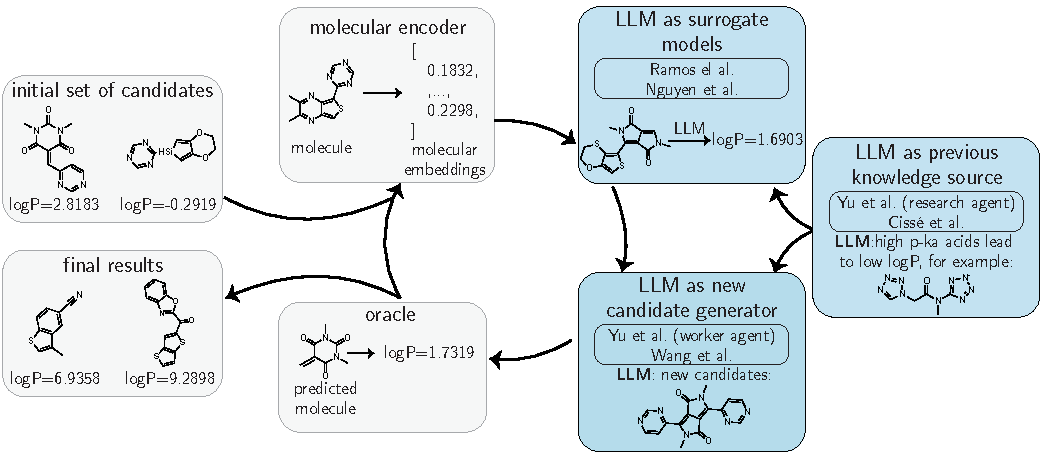
\includegraphics[width=1\textwidth]{figures/rescaled_figures/chemrev_figure22.pdf}
    \caption{\textbf{Overview of the iterative optimization loop that mirrors the structure of the optimization section}. The blue boxes contain the different roles that the \glspl{llm} play in the loop, and which are described in the main text. References in which the use of \glspl{llm} for that step are detailed inside the small boxes inside each of the components of the loop. The example shown is about obtaining molecules with high \texttt{logP}.}
    \label{fig:optimization}
\end{figure}

Discovering novel compounds and reactions in chemistry and materials science has long relied on iterative trial-and-error processes rooted in existing domain knowledge \autocite{Taylor2023brief}. While, as explained in \Cref{sec:retrosynthesis}, those methods are used to accelerate this process, optimization methods help improve conditions, binding affinity, etc.
But these approaches are slow and labor-intensive. 
Traditional data-driven methods aimed to address these limitations by combining predictive \gls{ml} models with optimization frameworks such as \gls{bo} or \glspl{ea}. 
These frameworks balance exploration of uncharted regions in chemical space with exploitation of known high-performing regions \autocite{Li2024sequential, Hse2021gryffin, Shields2021bayesian, Griffiths2020constrained, RajabiKochi2025adaptive}.

Recent advances in \glspl{llm} have unlocked potential for addressing optimization challenges in chemistry and related domains \autocite{fernando2023promptbreeder0, yang2023large, chen2024instruct}. 
A key strength of \glspl{llm} lies in their capacity to frame optimization tasks through natural language, which enhances knowledge incorporation, improves candidate comparisons, and increases interpretability. 
This aligns well with chemical problem-solving, where complex phenomena, such as reaction pathways or material behaviors, are often poorly captured by standard nomenclature; however, they can still be intuitively explained through natural language. 
Moreover, \glspl{gpm}' general capabilities provide flexibility beyond classical methods, which have to be trained from scratch if the optimization problem or any of its variables changes.
By encoding domain-specific knowledge---including reaction rules, thermodynamic principles, and structure-property relationships---into structured prompts, \glspl{llm} can synergize expertise with their ability to navigate complex chemical optimization problems.

Current \gls{llm} applications in chemistry optimization vary in scope and methodology. 
Many studies integrate \glspl{llm} into \gls{bo} frameworks, where models guide experimental design by predicting promising candidates \autocite{rankovic2023bochemian}. Others employ \glspl{ga} or hybrid strategies that combine \gls{llm}-generated hypotheses with computational screening \autocite{cisse2025language0based}.  

\subsubsection{LLMs as Surrogate Models}

A prominent \gls{llm}-driven strategy positions these models as surrogate models within optimization loops. Typically implemented as \gls{gpr}, surrogate models learn from prior data to approximate costly feature-outcome landscapes, which are often computationally and time-consuming to evaluate, thereby guiding the acquisition.
\glspl{llm} offer major advantages in this role primarily through strong low-data performance. 
Their \gls{icl} capability enables task demonstration with minimal prompt examples while leveraging chemical knowledge from pre-training to generate accurate predictions. 
This allows \glspl{gpm} to compensate for sparse experimental data effectively.

\textcite{ramos2023bayesian} demonstrated the viability of this paradigm through a simple yet effective framework that combines \gls{icl} using only one example in the prompt with a \gls{bo} workflow. 
Their \gls{bo}-\gls{icl} approach uses few-shot examples formatted as question-answer pairs, where the \gls{llm} generates candidate solutions conditioned on prior successful iterations. 
These candidates are ranked using an acquisition function, with top-$k$ selections integrated into subsequent prompts to refine predictions iteratively. 
Remarkably, this method achieved high performance in optimizing catalytic reaction conditions, even matching the top-1 accuracies observed in experimental benchmarks. This emphasizes the potential of \glspl{llm} as accessible, \gls{icl} optimizers when coupled with well-designed prompts.

To address limitations in base \glspl{llm}’ inherent chemical knowledge---particularly their grasp of specialized representations like \gls{smiles} or structure-property mappings---\textcite{yu2025collaborative} introduced a hybrid architecture augmenting pre-trained \glspl{llm} with task-specific embedding and prediction layers. 
These layers, fine-tuned on domain data, align latent representations of input-output pairs (denoted as \texttt{<x>} and \texttt{<y>} in prompts), enabling the model to map chemical structures and properties into a unified, interpretable space. Crucially, the added layers enhance chemical reasoning without sacrificing the flexibility of \gls{icl}, allowing the system to adapt to trends across iterations, similarly to what was done by \textcite{ramos2023bayesian}. 
In their evaluations of molecular optimization benchmarks, such as the \gls{pmo} \autocite{gao2022sample}, they revealed improvements over conventional methods, including \gls{bo}-\gls{gp}, \gls{rl} methods, and \gls{ga}.

\textcite{yu2025collaborative} further highlighted the framework’s extensibility to diverse black-box optimization challenges beyond chemistry. 
This represents one of the most important advantages of using \glspl{llm} as orchestrators of the optimization process. 
The flexibility of natural language in this process enables the procedure to be applied to any optimization process. 
In contrast, classical methods are constrained to the specific task for which they are designed due to the need to train the surrogate model.

\subsubsection{LLMs as Next Candidate Generators}

Recent studies demonstrate the potential of \glspl{llm} to enhance \glspl{ea} \autocite{lu2024generative} and \gls{bo} \autocite{amin2025towards} frameworks by leveraging their embedded chemical knowledge and ability to integrate prior information, thereby reducing computational effort while improving output quality.
Within \glspl{ea}, \glspl{llm} refine molecular candidates through mutations (modifying molecular substructures) or crossovers (combining parent molecules). 
In \gls{bo} frameworks, they serve as acquisition functions, utilizing surrogate model predictions---both mean and uncertainty---to select optimal molecules or reaction conditions for evaluation.

For molecule optimization, \textcite{yu2025collaborative} introduced \modelname{MultiModel}, a dual-\gls{llm} system where one model proposes candidates and the other supplies domain knowledge (see \Cref{sec:opt-llm-know-source}). 
By fine-tuning the \enquote{worker} \gls{llm} to recognize molecular scaffolds and target properties, and expanding the training pool to include a million-size pre-training dataset, they achieved hit rates exceeding $90\%$. 
Similarly, \textcite{wang2024efficient} developed \modelname{MoLLEO}, integrating an \gls{llm} into an \gls{ea} to replace random mutations with \gls{llm}-guided modifications. Here, \modelname{GPT-4} generated optimized offspring from parent molecules, significantly accelerating convergence to high fitness scores. 
Notably, while domain-specialized models (\modelname{BioT5}, \modelname{MoleculeSTM}) underperformed, the general-purpose \modelname{GPT-4} excelled---a finding that underscores the context-dependent utility of \glspl{llm}

In a related approach, \textcite{lu2024generative} showed that well-designed prompts---incorporating task-specific constraints, objectives, and few-shot examples---enable general \glspl{llm} (\modelname{Claude\--3.5-Sonnet}, \modelname{o1-preview}) to generate high-quality candidates without fine-tuning, outperforming both random selection and vanilla \glspl{ga} in functional \gls{tmc} design.

\subsubsection{LLMs as Prior Knowledge Sources} \label{sec:opt-llm-know-source}

A key advantage of integrating \glspl{llm} into optimization frameworks is their ability to encode and deploy prior knowledge within the optimization loop. 
As illustrated in \Cref{fig:optimization}, this knowledge can be directed into either the surrogate model or candidate generation module, significantly reducing the number of optimization steps required through high-quality guidance.

For example, \textcite{yu2025collaborative} deployed a \enquote{research} agent that leverages \modelname{Google} search and \modelname{RDKit} to verify and rank molecules generated by \enquote{worker} agents against target features and properties. 
Their results demonstrate substantial improvements when this filtering mechanism is applied.

Similarly, \textcite{cisse2025language0based} introduced \modelname{BORA}, which contextualizes conventional black-box \gls{bo} using an \gls{llm}. \modelname{BORA} maintains standard \gls{bo} as the core driver but strategically activates the \gls{llm} when progress stalls. 
This leverages the model’s \gls{icl} capabilities to hypothesize promising search regions and propose new samples, regulated by a lightweight heuristic policy that manages costs and incorporates domain knowledge (or user input). 
Evaluations on synthetic benchmarks such as the catalyst optimization task for hydrogen generation show that \modelname{BORA} accelerates exploration, improves convergence, and outperforms existing \gls{llm}-\gls{bo} hybrids.

To enhance the task-specific knowledge of the \gls{llm} generating feedback, \textcite{zhang2025large} fine-tuned a \modelname{Llama-2-7B} model using a multitask \gls{qa} dataset. This dataset was created with instructions from \modelname{GPT-4}. 
The resulting model served as a human assistant or operated within an active learning loop, thereby accelerating the exploration of new reaction spaces (see \Cref{sec:retrosynthesis}). 
However, as the authors note, even this task-specialized \glspl{llm} produces suboptimal suggestions for optimization tasks. 
They remain prone to hallucination and cannot assist with unreported reactions, but still, they improve for most of the applications, using pure classical methods.

\subsubsection{How to Face Optimization Problems?}

Published works explore different ways of using \glspl{llm} for optimization problems in chemistry, from simple approaches, such as just prompting the model with some initial random set of experimental candidates and iterating \autocite{ramos2023bayesian}, to fine-tuning models in \gls{bo} fashion \autocite{rankovic2025gollum0}. 
The most efficient initial point is by relying entirely on a \gls{icl} approach, which allows one to obtain a first signal rapidly. 
Such initial results will enable to determine whether a more complex, computationally intensive approach is necessary or whether prompt engineering is reliable enough for the application. 
Fine-tuning can be used as a way to enhance the chemical knowledge of the \glspl{llm} and can lead to improvements in optimization tasks where the model requires such knowledge to choose or generate better candidates. 
Fine-tuning might not be a game-changer for other approaches that rely more on sampling methods \autocite{wang2025llm0augmented}.

While some initial works showed that \glspl{llm} trained specifically on chemistry perform better for optimization tasks \autocite{kristiadi2024sober}, other works showed that a \gls{gpm} such as \modelname{GPT-4} combined with an \gls{ea} outperformed all other models \autocite{wang2024efficient}.
Is it better to incorporate a general model or a chemistry \gls{lm} into the optimization frameworks?
We hypothesize that for models of the same size (in number of parameters) and similar training size---attending to \glspl{pflop}---a chemical \gls{lm} (a specialized model) will consistently outperform general models. 
If the models differ significantly in size, the larger model will typically perform better.


\section{Implications of GPMs: Education, Safety, and Ethics}
\label{sec:implications}

The advent of \glspl{gpm} in the chemical sciences marks a paradigm shift that extends beyond methodological advances to fundamentally alter the conceptual frameworks through which scientific knowledge is produced and validated. 
As these models permeate education and research, their transformative potential is closely linked to critical challenges in cultivating discerning learners, mitigating emergent risks in automated discovery, and navigating ethical dilemmas arising from biased systems. 
Here, these tripartite implications are examined, and it is argued that responsible integration of \glspl{gpm} requires not only technical innovation but also rigorous pedagogical and regulatory frameworks.


\subsection{Education} \label{sec:education}

\subsubsection{Vision}

\glspl{gpm} are opening up new directions to create or use educational materials (see \Cref{fig:education}). 
Although many current applications are still in their conceptual stage, they begin to highlight the potential of these models to personalize learning, increase the fairness of evaluations, and improve accessibility. 
\glspl{gpm} can support both students and educators at various stages of the learning process and across different media forms, indicating a shift toward more adaptive and personalized educational frameworks. \autocite{Mollick2024}

For students, \glspl{gpm} could act as intelligent companions in a variety of tasks. 
As adaptive tutors, they could tailor explanations, exercises, and feedback to individual needs. 
Additionally, they could help students rehearse for exams and presentations and deepen their conceptual understanding. \autocite{mollick2024instructors, Sharma2025role, wang2025effect}

\begin{figure}[htb]
    \centering
    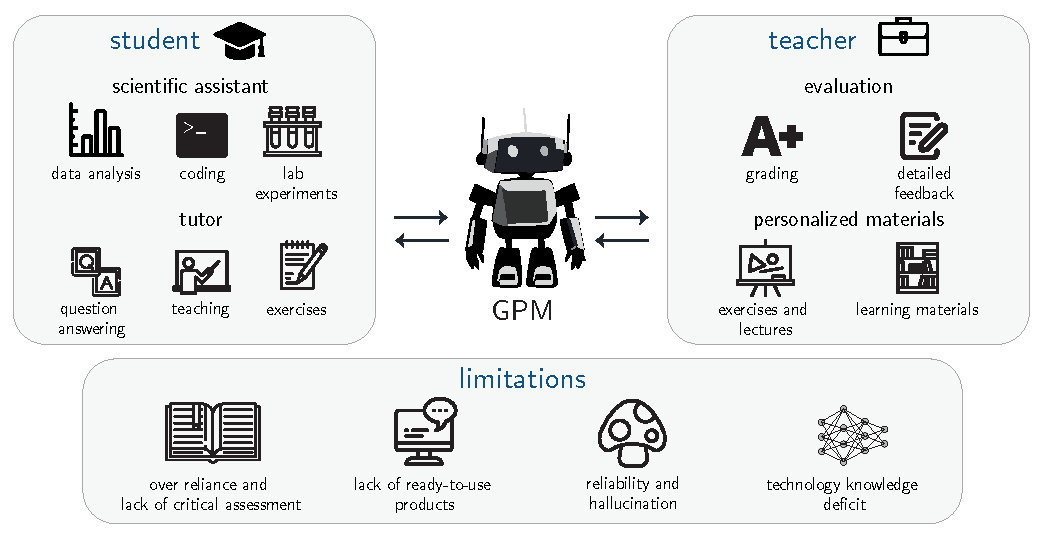
\includegraphics[width=1\linewidth]{figures/rescaled_figures/chemrev_figure23.pdf}
    \caption{\textbf{Possible application examples for students and teachers and their specific limitations for \glspl{gpm} in chemical education.} \glspl{gpm} can be used by students as scientific assistants (e.g., for data analysis, coding or lab experiments) and tutors (e.g., for question answering, teaching or exercises). Teachers can use \glspl{gpm} for evaluation (e.g., for grading and detailed feedback) or to personalize materials (e.g., for lectures and other learning materials). Current limitations include an over-reliance and a lack of critical assessment of the outputs, a lack of ready-to-use products, hallucination, a lack of reliability of the models, and a technology knowledge deficit of the users.}
    \label{fig:education}
\end{figure}

In more practice-oriented settings, such as laboratories or coding environments, these models could function as scientific assistants. They may provide real-time feedback on experimental setups, assist with how to use lab equipment, or help identify potential safety concerns.\autocite{Du2024} 
Coupled with \gls{ar}, \glspl{gpm} could also enable immersive simulations of lab procedures, allowing students to familiarize themselves with workflows and instruments before entering a physical lab. 
Moreover, by supporting students in technical areas such as coding, data analysis, or simulations, they could reduce the entry barrier or learning curve and thus foster interdisciplinary competence---particularly in contexts where instructor support is limited.

At the same time, \glspl{gpm} could ease the workload of educators. 
They offer new possibilities for generating and adapting course materials---ranging from lecture slides and exercises to individualized exam questions---thus enabling a better alignment with diverse learning levels and prior knowledge. In assessment tasks, these models could support the grading of open-ended responses by providing consistent, criteria-based feedback and reducing subjective bias.\autocite{Kortemeyer2024, gao2024towards} This is especially valuable in large courses or when timely, detailed feedback would otherwise be difficult to provide. 


\subsubsection{Current Status}

Despite these envisioned potentials of \glspl{gpm} in chemistry education, current applications are often still fragmented and lack integration into cohesive educational systems. 
In many cases, models are used via general-purpose interfaces without subject-specific customization or alignment with curricular goals. 
Rather than being part of purpose-built tools or platforms, their use remains largely exploratory.

\paragraph{General Systems}
Early applications often rely on zero-shot prompting of general-purpose \glspl{llm} or \glspl{vlm} to aid with student-oriented learning tasks. 
These include plotting data \autocite{Subasinghe2025}, writing code \autocite{Tsai2023}, or generating analogies to explain abstract chemical concepts \autocite{shao2025unlocking}. 

\textcite{handa2025education} analyzed over 570,000 anonymized Claude.ai conversations from university-affiliated users, finding that students primarily used the model for preparing learning materials ($39.3\%$) and solving academic problems ($33.5\%$). 
However, their use was often exploratory and low-stakes, and the study emphasizes the need for guidance, as many users lacked the expertise to evaluate model outputs critically.

Two recent studies have explored zero-shot prompting in more realistic, assessment-focused settings. \textcite{baral2025drawedumath0} introduced a benchmark of more than 2,000 student-drawn math images and found that state-of-the-art \glspl{vlm}, including \modelname{GPT-4o} and \modelname{Claude 3.5}, struggled to assess student reasoning and correctness, particularly in open-ended or diagram-based answers. 
Similarly, \textcite{Kortemeyer2024} investigated the use of \modelname{GPT-4} for grading handwritten thermodynamics exams at \modelname{ETH Zürich}. While the model performed reasonably well on short derivations, it failed to track detailed rubrics or interpret hand-drawn diagrams reliably. 
In chemistry education, \textcite{kharchenko2024advantages} compared \modelname{ChatGPT 3.5}, \modelname{Gemini}, and \modelname{Copilot} on domain-specific tasks and found that while the models performed adequately on simple recall questions, they failed in tasks that required chemical reasoning, structural understanding, or logical analysis.

Together, these findings suggest that while zero-shot prompting enables rapid deployment of \glspl{gpm} in educational contexts, current models lack the reliability, consistency, and domain grounding required for chemistry education---not only from a pedagogical standpoint, but also from ethical and legal perspectives.

\paragraph{Specialized Systems}
A growing number of applications embed \glspl{gpm} in specialized educational systems that combine \glspl{gpm} with structured components such as \gls{rag}, tracking learning progress, or the ability to work with multiple sources of content such as textbooks, lecture slides, or handwritten notes.

For example, \textcite{perez2025large} presented a biology \gls{qa} system that used a \gls{rag} pipeline to deliver curriculum-aligned answers. 
The I-Digest team \autocite{Jablonka2023} introduced a platform that generates lecture summaries and follow-up questions to support continuous learning. 
Some systems also integrate specialized components to improve personalization and continuity in the learning process. 
Although not designed for chemistry specifically, general-purpose platforms such as TutorLLM \autocite{li2025tutorllm0} (generating personalized content based on the learning progress) and LearnMate \autocite{wang2025learnmate0} (creating learning plans and giving feedback) demonstrate how large models can be embedded in structured educational frameworks. 

Anthropic's Claude for Education \autocite{AnthropicEducation} offers a purpose-built platform for higher education with a \enquote{Learning Mode} that uses the Socratic method to guide students rather than directly giving the answer to their queries. The intention here is to promote active learning and mitigate the risks of passive tool use. 
While such systems illustrate the potential of structured \gls{gpm}-based learning environments, fully integrated applications remain rare---particularly in domain-specific contexts such as chemistry. 
Furthermore, current models must still strengthen their robustness and domain-specific reasoning before they can be trusted in demanding fields, including chemistry.

\subsubsection{Outlook and Limitations}

While \glspl{gpm} offer promising opportunities for chemistry education, their use also raises critical ethical and pedagogical concerns.

A first concern is the lack of transparency in how these models generate responses. 
Although \glspl{gpm} produce fluent and plausible explanations, they do so without genuine understanding---and often with no clear indication of uncertainty or possible errors. 
This can lead students to accept incorrect or misleading information as fact, particularly when the output appears confident or authoritative. Over time, such interactions may normalize uncritical acceptance and discourage students from questioning, verifying, or reflecting on what they are told. 
In scientific education, where reasoning, skepticism, and an evidence-based mindset are essential, this poses a serious threat to the development of informed and independent   learners.\autocite{marcus2025will, kosmyna2025your}

A related but distinct issue is the risk of over-reliance and deskilling. When students delegate a large portion of the learning process to generative tools, they might be able to complete assignments without engaging in the mental work needed to develop subject-specific competence. 
In such cases, \glspl{gpm} can disrupt the connection between concrete tasks---such as solving a problem or writing an explanation---and the broader educational goals they are meant to support, such as developing chemical understanding or analytical thinking skills.\autocite{dung2025learning, Sharma2025role}

Today---and even more so in the future---students and learners will increasingly use \glspl{gpm}, both in education and in their future professions. 
Attempting to restrict their use is neither realistic nor educationally meaningful. 
Therefore, educators must guide their use thoughtfully and adapt both the learning process and assessment practices accordingly. 
Furthermore, the question of what to learn needs to be redefined. 
What we learn must increasingly center around the development of critical thinking, creativity, and logical reasoning---skills that remain essential and irreplaceable, even---or perhaps especially---in the age of \glspl{gpm}. \autocite{klein2025rethink}

\subsection{Safety} \label{sec:safety}

\begin{figure}[!htbp]
    \centering
    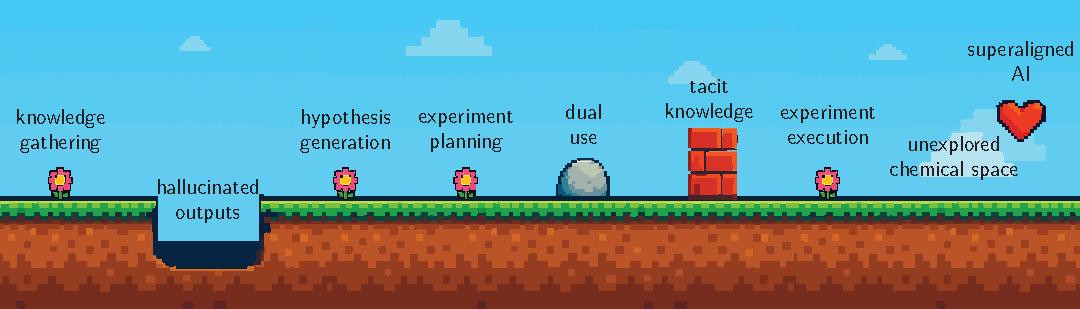
\includegraphics[width=1\linewidth]{figures/safety_chemrev_fig.pdf}
    \caption{\textbf{A conceptual schematic depicting \gls{ai} risk factors in chemical science}. As one traverses through the game-like scientific process, there are various obstacles to encountering \gls{ai} exacerbated risks. The path to superaligned chemical \gls{ai}-assistants is obfuscated by unexplored chemical space.}
    \label{fig:safety-overview}
\end{figure}

\noindent A growing coalition within the scientific community has sounded a call to action: \gls{ai} poses existential risks that deserve the same urgent attention as pandemics and nuclear war \autocite{cais2023statement}. 
This call, formalized in a statement signed by hundreds of prominent \gls{ai} researchers, reflects mounting recognition that advanced \gls{ai} systems could fundamentally alter, or threaten, human civilization. 
While the ongoing discourse has focused on abstract notions of \gls{agi}, the immediate risks may emerge through the integration of \gls{ai} into specific domains where the stakes are already high \autocite{morris2023levels}.

Chemistry represents one such domain. 
The rapid integration of \glspl{gpm} in chemistry is a dual-edged sword. 
Although these technologies can accelerate discovery, they also introduce unprecedented risks. 
From democratizing access to hazardous chemical knowledge to enabling autonomous synthesis of dangerous compounds, \gls{ai} systems could lower barriers for misuse, whether intentional or accidental. 
\glspl{gpm} alone may not create new risks \autocite{peppin2024reality}, but they can amplify existing ones (see \Cref{fig:safety-overview}).

Even in this amplified context, the ability of these systems to pose meaningful safety risks in practice is constrained by real-world limitations, including access to specialized lab equipment, regulated or scarce reagents, and, most critically, the \enquote{tacit knowledge}\autocite{Polanyi_2009} required to execute complex chemical processes. 
Tacit knowledge, the expertise gained through hands-on experience and intuition, cannot be fully acquired from textbooks or datasets alone, as it is normally shared verbally and encompasses small learnings, often considered insignificant. 
This gap between theoretical \gls{ai} outputs and practical execution underscores why risks, though serious, might remain manageable with proactive safeguards.

Ultimately, mitigating these threats requires a nuanced balance of fostering innovation while embedding safety at the architectural, operational, and governance levels.

\subsubsection{Evaluating Risk Amplification in the Chemical Discovery Cycle}

\paragraph{Dual Use} A critical question is whether \glspl{llm} provide maliciously acting novices with new avenues to obtain harmful knowledge beyond what is already easily accessible (e.g., via the internet)\autocite{sandbrink2023artificial}. 
Preliminary research has explored whether \glspl{llm} can exacerbate biorisks, a concern that extends analogously to chemical safety under the \enquote{information access} threat model \autocite{peppin2024reality}. \textcite{urbina2022dual} explored how their de novo molecular generator, \modelname{MegaSyn}, could be used to design toxic chemical agents by adjusting the reward system of the model to prefer compounds with greater toxicity and bioactivity. 
While their model predicted VX (toxic nerve agent) and other chemical warfare agents, the actual synthesis of such compounds requires expertise, controlled precursors, and specialized equipment that is far beyond the capabilities of most non-state actors.

Recent evaluations by \modelname{OpenAI} and \modelname{Anthropic} have systematically assessed how their models can facilitate the creation of biological threats. 
In an evaluation of their Deep Research System (a multi-agent architecture), \modelname{OpenAI} classified the system to be medium-risk for chemical and biological threat-creation. \autocite{openai2024building} 
As discussed previously, a key barrier that prevents such models from exceeding the assessed risk threshold is the acquisition of \enquote{tacit knowledge}. 
However, this system demonstrated modest improvements in troubleshooting and the acquisition of tacit knowledge. 
Although it still fell short of expert-level performance, these findings suggest that models are making progress toward overcoming this critical hurdle.
They also evaluated \modelname{GPT-4}'s impact on experts and students across five biological threat creation stages: ideation, acquisition, magnification, formulation, and release. \autocite{openai2024building} 
Their key finding was that biorisk information is widely accessible without \gls{ai} and that practical constraints such as wet lab access or domain expertise are more limiting than information scarcity. 

\modelname{Anthropic}'s parallel assessment of \modelname{Claude 4 Opus} focused specifically on biological risks through red-teaming with bio-defense experts, multi-step agentic evaluations, and explicit testing of bioinformatics tool integration \autocite{anthropic2025system}. 
Their findings align with \modelname{OpenAI}'s assessment of \modelname{GPT-4}, and conclude that current systems remain constrained by physical barriers. Both studies emphasize that supply chain control of chemicals, the flow of goods (e.g., chemical reagents) from suppliers to consumers, remains crucial as these systems continue to evolve and barriers to accessing knowledge are continuously lowered. For example, although \textcite{he2023control} showed that \glspl{llm} can generate pathways for explosives like \gls{petn} or nerve agents like sarin, the supply chain of obtaining precursor chemicals for weapons like sarin is tightly regulated. 
In addition, access to lab infrastructure like fume hoods or inert environments is not trivial to obtain for non-experts.

In the status quo it remains true that these risks are mitigated by material and logistical hurdles \autocite{sandbrink2023artificial}. Nonetheless, existing information access or presumed barriers to accessing materials are not an argument for \gls{ai} complacency. 
Models that lower the technical or cognitive barriers to weaponization even incrementally risk acting as force multipliers for malicious actors. 
Moreover, a red-teaming (discussed in \Cref{para:red_teaming}) effort proved that these practical constraints are circumventable and show that real world checks are prone to failure.

\paragraph{Hallucinations} Another critical risk of \glspl{gpm} is their propensity for hallucination, leading to factually incorrect outputs.\autocite{pantha2024challenges, ji2023survey}
These errors risk propagating misinformation, such as inventing non-existent chemical reactions or falsifying safety protocols. 
Additionally, \glspl{llm} suffer from temporal misalignment; their static training data renders outputs obsolete in fast-evolving fields like drug discovery \autocite{pantha2024challenges}. Therefore, their accuracy in chemistry decays sharply for research published after the training cutoff, underscoring the need for real-time verification systems.

\paragraph{Indirect Cyberattack Risk} The convergence of individual steps of the chemical discovery cycle in autonomous laboratory systems or cloud-based laboratories represents a high-risk scenario \autocite{rouleau2025risks}.
Beyond traditional cybersecurity threats, these systems face a critical timeline mismatch: \gls{ai} systems are projected to achieve superhuman hacking capabilities by 2027 while operating within inadequately secured infrastructure \autocite{dean2025security}. 
For autonomous laboratories, this means \gls{ai} systems capable of designing hazardous compounds could be compromised by external actors.

\subsubsection{Existing Approaches to Safety} Adversarial testing and red teaming have become prominent methods for evaluating the safety of \gls{ai} systems, even in the chemical domain (see \Cref{sec:evals}). 
While such evaluations are valuable to identify weaknesses in \glspl{gpm}, they are inherently reactive. 
These approaches highlight failures only after a model is trained or deployed, rather than embedding safety into the model's architecture. 
Moreover, adversarial testing is often unsystematic and relies on human-curated test cases that may not range across all potential risks, particularly in complex domains such as chemistry.

To move beyond reactive measures, an emerging field of safety research explores machine \enquote{unlearning}, a technique that selectively removes hazardous knowledge from a model's training data \autocite{barez2025open}. 
However, this approach faces significant challenges in chemistry. First, defining \enquote{dangerous chemical knowledge} is non-trivial because chemical properties are context-dependent.
Seemingly benign compounds like bleach can become hazardous when combined or misused. 
Second, unlearning risks can lead to a model's utility degradation, and the resulting challenge of balancing the trade-off between safety and functionality remains unresolved. 
This balance is especially challenging for \glspl{gpm}, which must achieve broad applicability with strict safety constraints.

A more implicit safety strategy is alignment, which aims to steer model behavior toward human values through techniques like \gls{rlhf} or Constitutional \gls{ai} \autocite{bai2022constitutional}. Although alignment can reduce harmful outputs, it may not generalize well to novel or domain-specific threats. 
For instance, a chemically aligned model might refuse to synthesize a known toxin, but could still be manipulated into suggesting precursor chemicals.  
Moreover, even after undergoing alignment training, they are still prone to produce risky and harmful content and will always be susceptible to jailbreaks \autocite{kuntz2025os-harm, yona2024stealing, lynch2025agentic}.

In an effort to train trustworthy models, many \gls{ai} researchers have turned to \enquote{interpretability}, an approach that aims to explain how the computations \glspl{gpm} are linked to the output. \autocite{cunningham2023sparse} 
However, in a recent global evaluation of \gls{ai} safety, \textcite{bengio2025international} argue that \gls{sota} interpretability tools have not proven their reliability in understanding models to modify them to alleviate safety risks.\autocite{makelov2023subspace}

\paragraph{Challenges in Developing Safeguards} Even chemistry-specific \glspl{llm} agents like \modelname{ChemCrow} \autocite{bran2024augmenting} or \modelname{Coscientist}\autocite{boiko2023autonomous} exhibit vulnerabilities. For instance, \modelname{ChemCrow}'s safeguards block known controlled substances, yet \textcite{he2023control} demonstrated a flaw in its safety protocols. 
The agent's refusals are reactive rather than proactive, as they rely on post-query web search checks rather than embedded safeguards. 

The capabilities and ensuing risks posed by \glspl{gpm} need to be contextualized around user intent \autocite{tang2024prioritizing}. 
Under a paradigm of malicious intent, the user intentionally creates a dangerous situation or application using the tool. 
However, an uninformed, benign user (e.g., a chemistry undergraduate student) could be unaware of the dangers posed by a given model output and unable to differentiate hallucinated responses. 

\subsubsection{Solutions}

The gaps in current \gls{ai} safety measures reveal a pressing need for proactive frameworks that address technical and systemic risks. \autocite{bengio2025international}

\paragraph{Regulatory Framework for Chemical \gls{ai} Models} Drawing from emerging biosecurity governance models, as a first step, chemical \gls{ai} oversight should focus on a narrow class of \enquote{advanced chemical models} that meet specific risk thresholds.  
Similar to proposed biological model regulations, these could include models trained on not widely accessible, particularly sensitive chemical data \autocite{bloomfield2024ai}. 
This targeted approach is preferable to regulating all chemical \gls{ai} models because it avoids creating compliance burdens that would disproportionately affect low-risk research while capturing the systems that actually pose security concerns.

\paragraph{Existing Institutional Efforts} Recent governmental initiatives have begun to address \gls{ai} safety concerns. 
The US \gls{ai} Safety Institute \autocite{nist2024safety} and the UK \gls{ai} Safety Institute have been tasked with designing safety evaluations for frontier models and researching catastrophic risks from \gls{ai} systems. 
In contrast, the \gls{eu} has taken a more pragmatic regulatory approach through the \gls{eu} \gls{ai} Act \autocite{EU2024regulation}, which classifies \gls{ai} systems by risk levels and imposes obligations ranging from transparency requirements to prohibited uses. 
These nascent efforts, while promising, face significant limitations. 
National institutes operate within frameworks that may prioritize domestic interests over global safety. 
While more comprehensive in scope, the \gls{eu} \gls{ai} Act focuses primarily on general \gls{ai} applications rather than domain-specific risks such as chemical synthesis, and its risk classification system may not adequately capture the unique dual-use nature of chemical \gls{ai} models.

\paragraph{Future Institutional Oversight and Transparency} A critical step forward is establishing neutral and independent regulatory bodies to oversee \gls{ai} development. 
Unlike self-regulation, which risks conflicts of interest, an \gls{iaio} comprised of \gls{ai} researchers, policymakers, ethicists, and security experts could harmonize standards and prevent a \enquote{race to the bottom} in regulatory laxity \autocite{trager2023international}. Such a body could mandate pre-approval for high-risk \gls{ai} research (like \gls{agi}-aligned projects), similar to institutional review boards that exist in the biomedical research space \autocite{pistono2016unethical}. Precedents for this exist in \gls{cern}, which tries to balance civilian duties with dual-use risks and nuclear non-proliferation treaties that tie market access to compliance.\autocite{cern_nuclear_safeguards_2024} 
Effective governance also requires binding enforcement mechanisms. 
One approach is conditional market access, where \gls{ai} products and precursors can only be traded internationally if certified by the \gls{iaio}. 
Participating states would then enact domestic laws to align with these standards, ensuring corporate and national compliance. 
This model leverages economic incentives rather than voluntary guidelines to enforce safety. Transparency must also be enforced, particularly in red-teaming and safety testing. 
Currently, many companies conduct red-teaming privately, with no obligation to disclose the findings or corrective actions.
To address this, \gls{ai} developers should be required to publicly report red-teaming results and undergo third-party safety audits for high-stakes applications.\autocite{carlini2025career}

The risks posed by \gls{ai} in chemistry demand immediate action from governments and institutions. 
Yet these challenges also invite a deeper question: \textit{Is the integration of \gls{ai} into scientific discovery fundamentally advancing our understanding or merely accelerating the production of epistemic noise?} 
As \textcite{narayanan2025why} cautioned, \gls{ai}’s predictive abilities often obscure its inability to explain underlying mechanisms. 
In chemistry, this tension is acute: \gls{ai}-driven tools may optimize reactions or design toxins with equal ease, but their black-box nature complicates accountability and obscures causal relationships. 
True progress may require safeguards against misuse and a reevaluation of whether \gls{ai}’s role in science should be expansive or deliberately constrained.

\subsection{Ethics} \label{sec:ethics}

The deployment of \glspl{gpm} in the chemical sciences raises several critical ethical concerns that require careful consideration. 
These issues range from perpetuating harmful biases to environmental impacts and intellectual property concerns \autocite{crawford2021atlas}.

\subsubsection{Environmental Impact and Climate Ethics}

The computational requirements for training and deploying \glspl{gpm} contribute to environmental degradation through excessive energy consumption and carbon emissions. \autocite{spotte-smith2025considering, nature2023carbon} 
These computational resources are often powered by fossil fuel-based energy sources, which directly contribute to anthropogenic climate change. \autocite{strubell2019energy} 
The emphasis on \gls{ai} research has superseded some of the commitments made by big technological companies to carbon neutrality. 
For example, Google rescinded its commitment to carbon neutrality amid a surge in \gls{ai} usage (65$\%$ increase in carbon emissions between 2021-24) and funding.\autocite{bhuiyan2025google} 
Additionally, the water consumption for cooling data centers that support these models is another concern, particularly in regions facing water scarcity. \autocite{mytton2021data}

The irony is particularly stark when considering that in the chemical sciences, these models are used to address climate-related challenges, such as the development of sustainable materials or carbon capture technologies. 
As a scientific community, we must grapple with the questions about the sustainability of current \gls{ai} development trajectories and consider more efficient and renewable approaches to model development and deployment. \autocite{kolbert2024obscene}


\subsubsection{Copyright Infringement and Plagiarism Concerns}

\glspl{gpm} are typically trained on a vast corpora of copyrighted scientific literature, patents, and proprietary databases, often without explicit permission, a practice that has sparked legal disputes, such as \textit{Getty Images v.\ Stability \gls{ai}}, where plaintiffs allege unauthorized scraping of protected content. \autocite{kirchhubel2024intellectual} Developers at \modelname{OpenAI} claimed in a statement to the \gls{uk} House of Lords that training \gls{sota} models is \enquote{impossible} without copyrighted material, highlighting a fundamental tension between \gls{ip} law and \gls{ai} advancement. \autocite{openai2023written} 
In the chemical sciences, this challenge persists through the training of models on experimental results from pay-walled journals. 
A potential resolution to this in the scientific sphere lies in the expansion of open-access research frameworks. 
Initiatives like the \gls{cas} Common Chemistry database provide legally clear training data while maintaining attribution.
\glspl{llm} have shown a high propensity to regurgitate elements from their training data. 
When generating text, models may reproduce near-verbatim fragments of training data without citation, effectively obscuring intellectual contributions.\autocite{bender2021dangers} 
While some praise \glspl{gpm} for overcoming \enquote{blank-page syndrome} for early-career scientists \autocite{altmae2023artificial}, others warn that uncritical reliance on their outputs risks eroding scientific rigor.\autocite{donker2023dangers}


\subsubsection{Bias and Discrimination}

\glspl{gpm} inherit and amplify harmful prejudices and stereotypes present in their training data, which pose significant risks when applied translationally to medicinal chemistry and biochemistry. \autocite{spotte-smith2025considering, yang2024demographic, omiye2023large} 
These models can perpetuate inaccurate and harmful assumptions based on race and gender about drug efficacy, toxicity, and disease susceptibility, leading to misdiagnosis and mistreatment. \autocite{chen2023algorithmic} 
Historical medical literature contains biased representations of how different populations respond to treatments, and \glspl{gpm} trained on such data can reinforce these misconceptions. \autocite{mittermaier2023bias}
The problem extends to broader contexts in chemical research. 
Biased models can influence research priorities, funding decisions, and the development of chemical tools in ways that systematically disadvantage the most vulnerable populations \autocite{dotan2019value0laden}. 

\paragraph{Solutions} The problem of bias can be best addressed through top-down reform. 
The data necessary to train unbiased models can only exist if clinical studies of drug efficacy are conducted on diverse populations in the real world.\autocite{criado-perez2019invisible} 
To complement improved data collection, standard evaluations for bias testing must be developed and mandated prior to deployment of \glspl{gpm}.


\subsubsection{Democratization of Power} 

Although \gls{ai} tools have the potential to democratize access to advanced chemical research capabilities, they may also concentrate power in the hands of a few large companies that control the frontier models. 
This concentration raises concerns about equitable access to research tools, particularly for researchers in smaller institutions with limited resources.\autocite{satariano2025a1i1}





\section{Outlook and Conclusions}
\begin{figure}[htb]
    \centering
    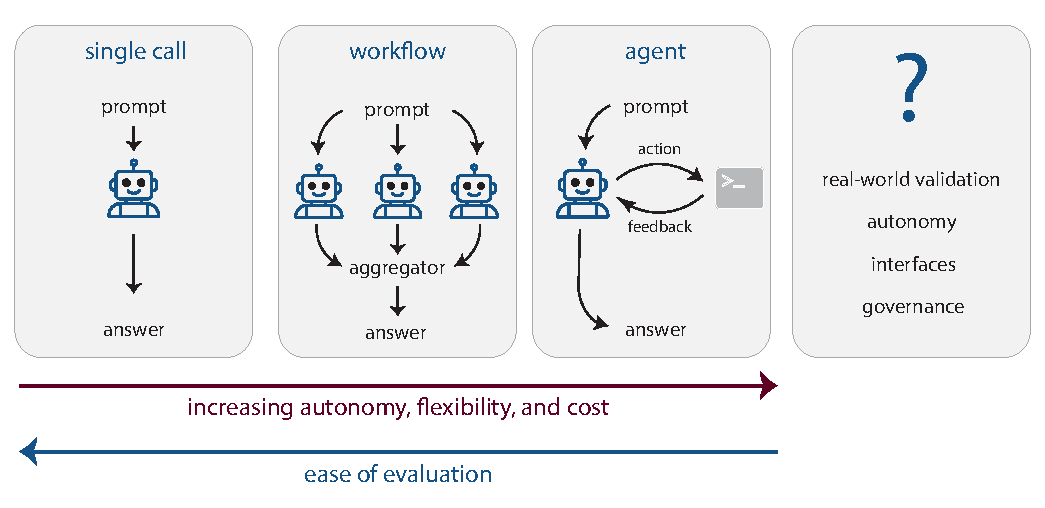
\includegraphics[width=1\linewidth]{figures/conclusion_figure_v2.pdf}
    \caption{\textbf{Evolution of \gls{gpm}-powered systems.} First \gls{gpm} applications directly used zero- or few-shot prompted or fine-tuned \glspl{gpm}. More complex tasks could be solved by combining multiple \glspl{gpm} in workflows where the execution trajectory is pre-determined. In agents, \glspl{gpm} autonomously decide on the execution trajectory and in this way enable researchers to address open-ended tasks. Moving forward, coupling the validation closer to real-world objectives with further increased validation in better, custom user interfaces will enhance the impact of \glspl{gpm}. To ensure safe and ethical deployment, the community must engage with the broader public and policymakers to devise governance strategies.}
    \label{fig:conclusions}
\end{figure}

As we have explored in this review, \glspl{gpm}---especially \glspl{llm}---hold remarkable promise for the chemical sciences. 
The field moved from using models in simple single calls to a \glspl{gpm} to developing workflows, in which a sequence of calls is performed, to increasingly complex autonomous agents in which the model decides on its own trajectory (see \Cref{fig:conclusions}). To power those agents, increasingly powerful models are being built, including reasoning models that promise higher data efficiency. 

Yet, several fundamental questions remain unresolved. We do not understand if there are fundamental limits to what can be predicted, given the inherent unpredictability of chemical systems and the reliance on tacit knowledge. We do not know what new datasets and techniques need to be developed, given the fact that the knowledge we extract from already published data is approaching a limit.\autocite{silver2025welcome} New data most likely will be generated by agents learning from their own experience.
To optimize systems, we need to better understand the underlying structure of chemical data.
In many other fields, data distributions have been shaped by special driving forces. 
For example, evolution led to a direct link between sequence and fitness in biological sequences, which makes such datasets special. In chemistry it is unclear what the \enquote{driving force} that shapes datasets is. 

It is also unclear how quickly these innovations will permeate the average chemistry lab, where the adoption of new technology depends on more than just predictive prowess. 
And we also do not know yet how we should interface with those models for the greatest effectiveness.
In addition, it is also unclear how far acceleration can take us, as nature imposes some natural speed limits: Some experiments simply take their time. 

Overall, this landscape suggests a future rich with opportunity. But realizing the potential impact of \glspl{gpm} demands clear-eyed caution: while it is now deceptively easy to spin up prototypes, transforming them into robust, reliable tools is a far more arduous task. \autocite{sculley2014machine}
More crucial still is our need for rigorous measurement and feedback---whether in the construction of evaluation suites, the calibration of reward functions for reinforcement learning, or the design of sensible governance. 
No single discipline can shoulder this alone; chemists, policy experts, and computer scientists must broaden their ranks and collaborate. 
This is particularly since science has always benefited from embracing a diversity of approaches. 
While \gls{gpm}-powered approaches for science, such as \enquote{AI scientists}, hold promise, a myopic focus on \enquote{AI scientists} might lead to \enquote{scientific monocultures}.\autocite{Savitsky_2025} 
We hope this review lowers the barrier to entry to the background and applications of \glspl{gpm} in the chemical sciences, inviting a wider spectrum of contributors to adopt a systems-science mindset---and, in doing so, to help harness the best of what \glspl{gpm} can offer for tackling the chemical sciences’ most persistent and pressing challenges.


\section*{Acknowledgments}

This work was supported by the Carl-Zeiss Foundation. 

\noindent A.A.\ acknowledges financial support for this research by the Fulbright U.S. Student Program, which is sponsored by the U.S. Department of State and the German-American Fulbright Commission. Its contents are solely the responsibility of the author and do not necessarily represent the official views of the Fulbright Program, the Government of the United States, or the German-American Fulbright Commission. 
 
\noindent M. S.-W.\ was supported by Intel and Merck via the AWASES research center. 

\noindent A.M.'s work was funded by the SOL-AI project, funded as part of the Helmholtz Foundation Model Initiative of the Helmholtz Association. 

\noindent G.P.'s work was supported by the HPC Gateway measure of the Helmholtz Association.


\noindent K.M.J.\ is part of the NFDI consortium FAIRmat funded by the Deutsche Forschungsgemeinschaft (DFG, German Research Foundation) – project 460197019.

\noindent We thank Mimi Lavin and Maximilian Greiner for their feedback on a draft of this article.

\section*{Author contributions}
N. A.\ was the primary contributor for the \enquote{Building principles of GPMs} section. Including its writing and figures (excluding the \enquote{adapting and using GPMs} subsection). N. A.\ also reviewed the \enquote{Introduction,} \enquote{Shape and structure of chemical data,} \enquote{Evals,} \enquote{Implication of GPMs,} and \enquote{Property prediction and material generation in accelerating applications} sections. \\

\noindent A. A.\ was the primary contributor to the \enquote{existing \glspl{gpm} for chemical science}, \enquote{property prediction}, \enquote{molecule and materials generation}, \enquote{retrosynthesis}, \enquote{safety}, and \enquote{ethics} sections, including their writing and figures. Edited introduction, evaluations, architectures, knowledge gathering, experiment execution, and education sections. \\ 

\noindent M.R.-G. was the primary contributor to the \gls{ai} scientist overview, the hypothesis generation, and the \gls{llm} as optimizers sections, and helped in reviewing the entire manuscript. \\

\noindent A.M.\ was the primary contributor to the introduction and data sections, and the main contributor to the knowledge gathering and reporting sections within the applications section, with minor contributions to the architecture and the safety sections. Has drafted the initial outline of the article. Reviewed the architecture sections, the safety section, the hypothesis generation, the data analysis sections and contributed to the review of the LLM-as-optimizers section.\\

\noindent M.S.-W.\ was the primary contributor to the evaluation, education and data analysis sections. M.S.-W. also reviewed the shape of chemical data, hypothesis generation, experiment execution, reporting and safety section. Unified all figures. Kept track of upcoming deadlines. \\ 

\noindent M.\ S.\ was the primary contributor to the writing of experimental planning section and related figure. And also helped in reviewing \enquote{Knowledge gathering,} \enquote{Property prediction,} and \enquote{LLMs as optimizers} sections. \\


\noindent G.P.\ was the primary contributor to the \enquote{Adapting and Using General Purpose Models} section, including its writing and table. G.P.\ additionally reviewed the \enquote{The Shape and Structure of Chemical Data,} \enquote{Data Analysis,} \enquote{Reporting} and \enquote{Molecular and Material Generation} sections. \\

\noindent A.A.A.\ was the primary contributor to the \enquote{Experiment Execution} section, including its figure, and a minor contributor to the post-training subsection. A.A.A.\ reviewed the \enquote{Introduction,} \enquote{Experiment Planning,} \enquote{Molecule/Materials Generation} and \enquote{Education} sections, edited \enquote{The Shape and Structure of Chemical Data} and part of \enquote{Building principles of GPMs} sections, created the glossary, and ensured that most references can be easily accessed via a DOI or URL. \\

\noindent K.M.J.\ initiated and led the project. K.M.J.\ edited all sections. 

\section*{Conflicts of Interest}
K.M.J.\ has been a paid contractor for OpenAI as part of the Red-Teaming Network.

\clearpage
\printbibliography

\clearpage
\glsaddall
\printnoidxglossary[type=\acronymtype, sort=letter]
\printnoidxglossary[type=main, title=Glossary]
\end{document}
 